% pdflatex -shell-escape software-analysis-main.tex
\documentclass[12pt,openany]{book}

\usepackage{kotex}
\usepackage{enumerate}
\usepackage{commath}
\usepackage{pifont} %http://ctan.org/pkg/pifont

\usepackage{stmaryrd} %llbracket
\usepackage{slantsc}
\usepackage{hyperref}
\usepackage{adjustbox}

\usepackage{array,booktabs}
\usepackage{multirow}
\usepackage{tabularx}


% Packages for formatting
%\usepackage[margin=1in]{geometry}
%\usepackage{fancyhdr}
%\usepackage{graphicx}
%\usepackage{amsmath}
%\usepackage{amsthm}
%%\usepackage{algorithm2e,setspace}
%\usepackage{algpseudocode}
%%\usepackage{xcolor}
%\usepackage{amssymb}
\usepackage{amsthm}

% Define custom theorem styles
\newtheoremstyle{dotless} % Name of the style
{3pt} % Space above
{3pt} % Space below
{\itshape} % Body font
{} % Indent amount
{\bfseries} % Theorem head font
{} % Punctuation after theorem head
{2.5mm} % Space after theorem head
{} % Theorem head spec

\newtheoremstyle{definitionstyle} % Name of the style
{3pt} % Space above
{3pt} % Space below
{} % Body font
{} % Indent amount
{\bfseries} % Theorem head font
{.} % Punctuation after theorem head
{2.5mm} % Space after theorem head
{} % Theorem head spec

% Applying custom styles
%\theoremstyle{dotless}
\newtheorem{theorem}{Theorem} % Theorem environment with section-wise numbering
\newtheorem*{theorem*}{Theorem} % Theorem environment with section-wise numbering
\newtheorem*{lemma*}{Lemma} % Theorem environment with section-wise numbering
\newtheorem*{proposition*}{Proposition} % Theorem environment with section-wise numbering
\newtheorem*{corollary*}{Corollary} % Theorem environment with section-wise numbering
\newtheorem{proposition}[theorem]{Proposition} % Theorem environment with section-wise numbering
\newtheorem{lemma}[theorem]{Lemma} % Lemma shares the counter with theorem
\newtheorem{corollary}[theorem]{Corollary} % Corollary shares the counter with theorem

\theoremstyle{definitionstyle}
\newtheorem*{observation}{\textcolor{magenta}{Observation}}
\newtheorem*{illustration}{\textcolor{teal}{Illustration}}
\newtheorem*{torus}{{\color{red}T}{\color{orange}o}{\color{green!75!black}r}{\color{cyan}u}{\color{violet}s}}
\newtheorem{definition}{Definition} % Definition shares the counter with theorem
\newtheorem{example}{Example} % Example shares the counter with theorem
\newtheorem{exercise}{{Exercise}} % Example shares the counter with theorem
\newtheorem{remark}{Remark} % Remark shares the counter with theorem
\newtheorem*{note}{Note}
\newtheorem*{notation}{Notation}

\newtheorem*{axiom*}{Axiom}
\newtheorem*{definition*}{Definition} % Definition shares the counter with theorem
\newtheorem*{example*}{Example} % Example shares the counter with theorem
\newtheorem*{exercise*}{\textcolor{teal}{Exercise}} % Example shares the counter with theorem
\newtheorem*{remark*}{Remark} % Remark shares the counter with theorem


\input{preambles/layout}
\usepackage{tcolorbox}
\tcbset{colback=white, arc=5pt}

\definecolor{axiomcolor}{HTML}{a88bfa}
\definecolor{defcolor}{RGB}{52, 152, 219}
\definecolor{procolor}{RGB}{241, 196, 15}
\definecolor{thmcolor}{RGB}{231, 76, 60}
\definecolor{lemcolor}{RGB}{155, 89, 182}
\definecolor{corcolor}{RGB}{46, 204, 113}
\definecolor{execolor}{RGB}{90, 128, 127}

% Define a new command for the custom tcolorbox
\newcommand{\axiombox}[2][]{%
	\begin{tcolorbox}[colframe=axiomcolor, title={\color{white}\bfseries #1}]
		#2
	\end{tcolorbox}
}

\newcommand{\defbox}[2][]{%
	\begin{tcolorbox}[colframe=defcolor, title={\color{white}\bfseries #1}]
		#2
	\end{tcolorbox}
}

\newcommand{\probox}[2][]{%
	\begin{tcolorbox}[colframe=procolor, title={\color{white}\bfseries #1}]
		#2
	\end{tcolorbox}
}

\newcommand{\thmbox}[2][]{%
	\begin{tcolorbox}[colframe=thmcolor, title={\color{white}\bfseries #1}]
		#2
	\end{tcolorbox}
}

\newcommand{\lembox}[2][]{%
	\begin{tcolorbox}[colframe=lemcolor, title={\color{white}\bfseries #1}]
		#2
	\end{tcolorbox}
}
\usepackage{tikz}
\usepackage{tikz-cd}
\usetikzlibrary{shadows}
\usetikzlibrary{shapes.geometric, arrows.meta, positioning}
\input{preambles/algorithm}
\input{preambles/listing}
\input{preambles/commands}

% ---------- Notation ----------
\newcommand{\CP}{\mathbb{CP}}
\newcommand{\M}{\mathcal{M}}

%\newcommand{\Z}{\mathbb{Z}}
\newcommand{\Ab}{\mathsf{Ab}}
\newcommand{\Mod}{\mathsf{Mod}}
\newcommand{\GL}{\operatorname{GL}}
\newcommand{\im}{\operatorname{im}}
\newcommand{\Ker}{\operatorname{Ker}}
\newcommand{\coker}{\operatorname{coker}}
\newcommand{\Hom}{\operatorname{Hom}}
\newcommand{\kk}{\Bbbk}
%\newcommand{\Z}{\mathbb{Z}}
%\newcommand{\im}{\operatorname{im}}
\newcommand{\rank}{\operatorname{rank}}
\newcommand{\nullity}{\operatorname{nullity}}
%\newcommand{\id}{\mathrm{id}}

\newcommand{\Om}{\Omega}
\newcommand{\dd}{\,\mathrm{d}}
\newcommand{\res}{\!\mid}
\newcommand{\dR}{\mathrm{dR}}
%\DeclareMathOperator{\im}{im}
%\DeclareMathOperator{\Ker}{Ker}
 \newcommand{\grad}{\nabla}
 \newcommand{\diver}{\operatorname{div}}
 \newcommand{\curl}{\operatorname{curl}}
 \newcommand{\flatop}{\flat}   % use v^\flat
 \newcommand{\sharpop}{\sharp} % use \alpha^\sharp
 \newcommand{\vol}{\operatorname{vol}}
 \newcommand{\X}{\mathfrak{X}(\mathbb{R}^3)}

\renewcommand{\emph}[1]{\textbf{#1}}

\begin{document}
\begin{titlepage}
    \centering
    
    \vspace*{1cm}
    
    \Huge\textsf{\textbf{Notes on Complex Analysis and
    		Riemann Surface Theory toward Algebraic Geometry}}
    
    \vspace{0.5cm}
%    \LARGE\textsf{- A Journey from Concretization to Abstraction -}
    
    \vspace{1.5cm}
    \textbf{Ji, Yonghyeon}

    \vfill
    A document presented for\\
    the Algebraic Geometry
    
    \vspace{0.8cm}
%    {\large\textsf{Department of Cyber Security}\par}
%    {\large\textsf{College of Science and Technology}\par}
%    {\large\textsf{Kookmin University}\par}
    \vspace{.25in}
    {\large \textsf{\today}\par}
    
%    \Large{Institution Name}\\
%    Date
\end{titlepage}


\tableofcontents
\newpage

\chapter{De Rham Complex, Short Exact Sequence, and Mayer-Vietoris}
\section{Grad / Curl / Div}

On $M=\R^3$ (with its standard Euclidean metric and orientation), the exterior derivative
packages the familiar vector calculus operators:

\begin{table}[h]
	\centering
	\renewcommand{\arraystretch}{1.35}
	\setlength{\tabcolsep}{10pt}
	\begin{tabular}{
		@{}>{\raggedright\arraybackslash}p{0.09\linewidth} |
		>{\raggedright\arraybackslash}p{0.225\linewidth} |
		>{\raggedright\arraybackslash}p{0.39\linewidth} |
		>{\raggedright\arraybackslash}p{0.225\linewidth}@{}
		}
		\toprule
		\textbf{Degree} & \textbf{Differential Form} & \textbf{Exterior derivative $d$} & \textbf{Vector calculus} \\
		\midrule
		\multirow{2}{*}{$0$-forms} &
		$f\in \Omega^0(\R^3)$ &
		$d:\Omega^0(\R^3)\to \Omega^1(\R^3),$
		& Gradient \\
		& (scalar field) & $df=f_x\,dx+f_y\,dy+f_z\,dz$
		& $df \;\leftrightarrow\; \nabla f$ \\ \hline
%		\addlinespace
		\multirow{2}{*}{$1$-forms} &
		$\alpha\in \Omega^1(\R^3)$, &
		$d:\Omega^1(\R^3)\to \Omega^2(\R^3),$ &
		Curl (via Hodge star)\\
		& $\alpha=P\,dx+Q\,dy+R\,dz$ 
		& $d\alpha=
		\Big(R_y-Q_z\Big)\,dy\wedge dz
		+\Big(P_z-R_x\Big)\,dz\wedge dx
		+\Big(Q_x-P_y\Big)\,dx\wedge dy$
		& $d\alpha \;\leftrightarrow\; \nabla\times (P,Q,R)$ \\ \hline
%		\addlinespace
		\multirow{2}{*}{$2$-forms} &
		$\beta\in \Omega^2(\R^3)$, &
		$d:\Omega^2(\R^3)\to \Omega^3(\R^3),$
		&
		Divergence
		\\
		& $\beta=A\,dy\wedge dz+B\,dz\wedge dx+C\,dx\wedge dy$ 
		& $d\beta=\big(A_x+B_y+C_z\big)\,dx\wedge dy\wedge dz$
		& $d\beta \;\leftrightarrow\; \nabla\cdot (A,B,C)$\\
		\bottomrule
	\end{tabular}
	\caption{On $\R^3$ (with Euclidean metric and orientation), the exterior derivative packages grad/curl/div (using the Hodge star to identify $2$-forms with vector fields).}
\end{table}

\begin{itemize}
	\item \textbf{Functions} $f\in\Om^0(\R^3)$ correspond to scalar fields.
	The map
	\[
	d:\Om^0(\R^3)\to \Om^1(\R^3)
	\]
	corresponds to the \textbf{gradient}:
	if $f=f(x,y,z)$ then
	\[
	df = \frac{\partial f}{\partial x}\,dx+\frac{\partial f}{\partial y}\,dy+\frac{\partial f}{\partial z}\,dz.
	\]
	Viewing $1$-forms as vector fields via the Euclidean metric, $df$ corresponds to $\nabla f$.
	
	\item \textbf{1-forms} $\alpha\in\Om^1(\R^3)$ correspond (after identifying $1$-forms with vector
	fields) to vector fields $\mathbf{F}=(P,Q,R)$ via
	\[
	\alpha = P\,dx + Q\,dy + R\,dz.
	\]
	Then
	\[
	d:\Om^1(\R^3)\to \Om^2(\R^3)
	\]
	corresponds to \textbf{curl}. Indeed,
	\[
	d\alpha
	= \left(\frac{\partial R}{\partial y}-\frac{\partial Q}{\partial z}\right)\,dy\wedge dz
	+ \left(\frac{\partial P}{\partial z}-\frac{\partial R}{\partial x}\right)\,dz\wedge dx
	+ \left(\frac{\partial Q}{\partial x}-\frac{\partial P}{\partial y}\right)\,dx\wedge dy,
	\]
	and (using the Hodge star to identify $2$-forms with vector fields) this corresponds to
	$\nabla\times \mathbf{F}$.
	
	\item \textbf{2-forms} $\beta\in\Om^2(\R^3)$ correspond (via the Hodge star) to vector fields
	$\mathbf{G}=(A,B,C)$ by writing
	\[
	\beta = A\,dy\wedge dz + B\,dz\wedge dx + C\,dx\wedge dy.
	\]
	Then
	\[
	d:\Om^2(\R^3)\to \Om^3(\R^3)
	\]
	corresponds to \textbf{divergence}:
	\[
	d\beta = \left(\frac{\partial A}{\partial x}+\frac{\partial B}{\partial y}+\frac{\partial C}{\partial z}\right)\,dx\wedge dy\wedge dz,
	\]
	which corresponds to $\nabla\cdot \mathbf{G}$.
\end{itemize}

\begin{table}[h]
	\centering
	\renewcommand{\arraystretch}{1.35}
	\setlength{\tabcolsep}{10pt}
	\begin{tabular}{
			@{}>{\raggedright\arraybackslash}p{0.125\linewidth} |
			>{\raggedright\arraybackslash}p{0.36\linewidth}
			>{\raggedright\arraybackslash}p{0.40\linewidth}@{}}
		\toprule
		\textbf{Operator} & \textbf{Differential form side} & \textbf{Vector field side (via $\flat,\sharp, *$)} \\
		\midrule
		Gradient &
		For $f\in C^\infty(\R^3)=\Omega^0(\R^3)$,
		\[
		df\in \Omega^1(\R^3)
		\]
		&
		Define $\grad f\in \mathfrak{X}(\R^3)$ by
		\[
		(\grad f)^\flat = df,\qquad
		\grad f = (df)^\sharp.
		\]
		\\
		\addlinespace
		Curl &
		For a vector field $X\in \mathfrak{X}(\R^3)$ with $1$-form $X^\flat\in\Omega^1(\R^3)$,
		\[
		d(X^\flat)\in \Omega^2(\R^3)
		\]
		&
		Define $\curl X\in \mathfrak{X}(\R^3)$ by
		\[
		(\curl X)^\flat = *\,d(X^\flat),\qquad
		\curl X = \big(*\,d(X^\flat)\big)^\sharp.
		\]
		\\
		\addlinespace
		Divergence &
		For a vector field $X\in \mathfrak{X}(\R^3)$,
		consider the $2$-form $*X^\flat\in\Omega^2(\R^3)$ and its derivative
		\[
		d(*X^\flat)\in\Omega^3(\R^3)
		\]
		&
		Let $\vol$ be the Euclidean volume form. Define $\diver X\in C^\infty(\R^3)$ by
		\[
		d(*X^\flat) = (\diver X)\,\vol,\quad
		\diver X = *\,d(*X^\flat).
		\]
		\\
		\bottomrule
	\end{tabular}
	\caption{Coordinate-free grad/curl/div on $(\R^3,g)$ using musical isomorphisms $\flat,\sharp$ and the Hodge star $*$.}
\end{table}

% ------------------------------------------------------------
% (Optional) one-line identities showing d^2=0 becomes curl grad=0, div curl=0
% ------------------------------------------------------------
\[
\curl(\grad f)
= \big(*\,d((df)^\sharp{}^\flat)\big)^\sharp
= \big(*\,d(df)\big)^\sharp = 0,
\qquad
\diver(\curl X)
= *\,d\big(*(\curl X)^\flat\big)
= *\,d\big(*(*\,d(X^\flat))\big)=0,
\]
where we used $d^2=0$ and $*^2=\pm 1$ on forms in dimension $3$.

%\subsection*{Why $d\circ d=0$ matches ``curl grad = 0'' and ``div curl = 0''}
The cochain condition $d^{k+1}\circ d^k=0$ becomes, under the above identifications,
\[
\nabla\times(\nabla f)=0
\qquad\text{and}\qquad
\nabla\cdot(\nabla\times \mathbf{F})=0.
\]
In general, the de Rham complex is the coordinate-free framework that explains these
vector calculus identities.

\subsection*{Cohomology as ``obstructions to being a gradient/curl''}
In $\R^3$, ``closed'' and ``exact'' specialize as follows:
\begin{itemize}
	\item A $1$-form $\alpha$ is \textbf{closed} iff $d\alpha=0$, i.e.\ $\nabla\times\mathbf{F}=0$
	(irrotational field). It is \textbf{exact} iff $\alpha=df$, i.e.\ $\mathbf{F}=\nabla f$.
	Thus $H^1_{\dR}$ measures irrotational fields that are not global gradients.
	\item A $2$-form $\beta$ is \textbf{closed} iff $d\beta=0$, i.e.\ $\nabla\cdot\mathbf{G}=0$
	(sourceless field). It is \textbf{exact} iff $\beta=d\alpha$, i.e.\ $\mathbf{G}=\nabla\times\mathbf{F}$.
	Thus $H^2_{\dR}$ measures divergence-free fields that are not global curls.
\end{itemize}
On contractible domains (like $\R^3$), the Poincar\'e lemma implies these obstructions vanish:
$H^k_{\dR}(\R^3)=0$ for $k\ge 1$.

\begin{figure}[h]
% ------------------------------------------------------------
% 1) The "big picture" correspondence diagram
% ------------------------------------------------------------
\[
\begin{tikzcd}[column sep=huge,row sep=large]
	\Om^0(\mathbb{R}^3)
	\arrow[r,"d"]
	&
	\Om^1(\mathbb{R}^3)
	\arrow[r,"d"]
	&
	\Om^2(\mathbb{R}^3)
	\arrow[r,"d"]
	&
	\Om^3(\mathbb{R}^3)
	\\
	C^\infty(\mathbb{R}^3)
	\arrow[u,equal]
	\arrow[r,"\grad"']
	&
	\X
	\arrow[u,"\flat"',shift right=0.8ex]
	\arrow[u,"\sharp",shift left=0.8ex]
	\arrow[r,"\curl"']
	&
	\X
	\arrow[u, "{(*\,\cdot)^\flat}"', shift right=0.8ex]
	\arrow[u, "{(*\,\cdot)^\sharp}",  shift left=0.8ex]
	\arrow[r,"\diver"']
	&
	C^\infty(\mathbb{R}^3)
	\arrow[u,"*^{-1}= \pm *"']
\end{tikzcd}
\]
\caption{Vector calculus operators as conjugates of $d$ via $\flat,\sharp,*$ in $\mathbb{R}^3$.}
\end{figure}

\vspace{1em}

% ------------------------------------------------------------
% 2) curl = ( * d (·)^flat )^sharp and curl(grad f)=0
% ------------------------------------------------------------
\[
\begin{tikzcd}[column sep=huge,row sep=large]
C^\infty(\mathbb{R}^3)
\arrow[r,"\grad"]
\arrow[d,equal]
&
\X
\arrow[r,"\curl"]
\arrow[d,"\flat"']
&
\X
\arrow[d,"\flat"']
\\
\Om^0(\mathbb{R}^3)
\arrow[r,"d"']
&
\Om^1(\mathbb{R}^3)
\arrow[r,"{*\,d}"']
&
\Om^1(\mathbb{R}^3)
\end{tikzcd}
\qquad\Rightarrow\qquad
\curl(\grad f)
= \big(*\,d(df)\big)^\sharp
= \big(*\,d^2 f\big)^\sharp
=0.
\]

\vspace{1em}

% ------------------------------------------------------------
% 3) div = * d * (·)^flat and div(curl X)=0
% ------------------------------------------------------------
\[
\begin{tikzcd}[column sep=huge,row sep=large]
\X
\arrow[r,"\curl"]
\arrow[d,"\flat"']
&
\X
\arrow[r,"\diver"]
\arrow[d,"\flat"']
&
C^\infty(\mathbb{R}^3)
\arrow[d,equal]
\\
\Om^1(\mathbb{R}^3)
\arrow[r,"d"']
&
\Om^2(\mathbb{R}^3)
\arrow[r,"{d}"']
&
\Om^3(\mathbb{R}^3)
\end{tikzcd}
\qquad\text{with}\qquad
\curl X = \big(*\,d(X^\flat)\big)^\sharp,\quad
\diver Y = *\,d\big(*\,Y^\flat\big).
\]
\[
\Rightarrow\quad
\diver(\curl X)
= *\,d\Big(*(\curl X)^\flat\Big)
= *\,d\Big(*(*\,d(X^\flat))\Big)
= \pm *\,d(d(X^\flat))
=0,
\]
where the sign comes from $*^2=\pm 1$ on $k$-forms in dimension $3$ (in Euclidean $\mathbb{R}^3$, $*^2=+1$ for all $k$).



\newpage
\section*{de Rham Cohomology}
\defbox[Cochain Complex]{
Let $M$ be a smooth manifold. A \emph{cochain complex} $(C^\bullet, d^\bullet)$ in $\R$-vector spaces consists of
\begin{itemize}
	\item $\R$-vector spaces $C^k$ for each $k\in\mathbb{Z}$,
	\item $\R$-linear maps (coboundary maps) $d^k: C^k \to C^{k+1}$,
\end{itemize}
such that $d^{k+1}\circ d^k = 0$ for all $k$.
}

\defbox[de Rham cochain complex]{
For a smooth manifold $M$, the de Rham cochain complex $(\Om^\bullet(M), d)$ is
\[
0 \to \Om^0(M) \xrightarrow{d} \Om^1(M) \xrightarrow{d} \Om^2(M) \xrightarrow{d} \cdots,
%\qquad d\circ d=0,
\] where \begin{itemize}
	\item $\Om^k(M)$ is the $\R$-vector space of smooth differential $k$-forms on $M$.
	\item $d^k := d:\Om^k(M)\to \Om^{k+1}(M)$ is the exterior derivative such that \[
	d^{k+1}\circ d^k = 0 \quad\text{for all } k\ge 0.
	\]
\end{itemize}
}

\subsection*{The de Rham complex as a cochain complex}
For a smooth manifold $M$, the de Rham cochain complex is
\[
0 \to \Om^0(M) \xrightarrow{d} \Om^1(M) \xrightarrow{d} \Om^2(M) \xrightarrow{d} \cdots,
\qquad d\circ d=0.
\]
In $\R^3$ (with a metric), $d$ corresponds to grad/curl/div after identifying vector fields with differential forms via the Hodge star.

\subsection*{De Rham cohomology}
\[
H^k_{\mathrm{dR}}(M)
:= \frac{Z^k(M)}{B^k(M)}
= \frac{\ker(d:\Om^k(M)\to \Om^{k+1}(M))}{\mathrm{im}(d:\Om^{k-1}(M)\to \Om^{k}(M))}.
\]
This measures global obstructions to writing a closed form as $d(\text{potential})$.

\subsection*{Short exact sequence (SES) of complexes for a cover $M=U\cup V$}
For each $k$ define
\[
\alpha^k:\Om^k(M)\to \Om^k(U)\oplus\Om^k(V),\quad \alpha^k(\omega)=(\omega\res_U,\omega\res_V),
\]
\[
\beta^k:\Om^k(U)\oplus\Om^k(V)\to \Om^k(U\cap V),\quad \beta^k(\eta,\theta)=\eta\res_{U\cap V}-\theta\res_{U\cap V}.
\]
Then (for smooth manifolds) one has a short exact sequence
\[
0\to \Om^k(M)\xrightarrow{\alpha^k}\Om^k(U)\oplus\Om^k(V)\xrightarrow{\beta^k}\Om^k(U\cap V)\to 0.
\]
Middle exactness $\mathrm{im}(\alpha^k)=\ker(\beta^k)$ is the gluing property (sheaf property); surjectivity of $\beta^k$ uses partition of unity.
Since $d$ commutes with restriction, these assemble into an SES of cochain complexes:
\[
0\to \Om^*(M)\xrightarrow{\alpha}\Om^*(U)\oplus\Om^*(V)\xrightarrow{\beta}\Om^*(U\cap V)\to 0.
\]

\subsection*{Mayer--Vietoris long exact sequence}
Any SES of cochain complexes yields a long exact sequence in cohomology:
\[
\cdots \to H^{k-1}(U\cap V)\xrightarrow{\delta} H^k(M)
\to H^k(U)\oplus H^k(V)\to H^k(U\cap V)\xrightarrow{\delta} H^{k+1}(M)\to \cdots
\]
The connecting map $\delta$ may be written explicitly using a partition of unity $\rho_U+\rho_V=1$:
for $d\eta=0$ on $U\cap V$,
\[
\delta([\eta])=\big[\,d(\rho_V\eta)\,\big]=\big[\,d\rho_V\wedge \eta\,\big]\in H^k(M).
\]

\bigskip
\begin{center}
	\begin{tikzcd}[column sep=large]
		0 \arrow[r] &
		\Om^*(M) \arrow[r,"\alpha"] &
		\Om^*(U)\oplus \Om^*(V) \arrow[r,"\beta"] &
		\Om^*(U\cap V) \arrow[r] & 0
	\end{tikzcd}
\end{center}

\newpage
\section{Example: The circle $S^1$}
\subsection{Cover and overlap}
Let \[
U=S^1\setminus\{(-1,0)\},\qquad V=S^1\setminus\{(1,0)\}.
\] Then $U,V$ are contractible; $U\cap V$ has two connected components $A$ (upper arc) and $B$ (lower arc).

\begin{center}
	\begin{tikzpicture}[scale=2.2, line cap=round, line join=round]
		% circle
		\draw[thick] (0,0) circle (1);
		% removed points
		\fill (-1,0) circle (0.03) node[left] {$(-1,0)$};
		\fill ( 1,0) circle (0.03) node[right] {$(1,0)$};
		
		% arcs highlighting overlap components (schematic)
		\draw[very thick, decoration={markings, mark=at position 0.5 with {\arrow{Stealth}}}, postaction={decorate}]
		(-1,0) arc[start angle=180, end angle=0, radius=1] node[pos=0.5, above=6pt] {$A\subset U\cap V$};
		\draw[very thick, decoration={markings, mark=at position 0.5 with {\arrow{Stealth}}}, postaction={decorate}]
		( 1,0) arc[start angle=0, end angle=-180, radius=1] node[pos=0.5, below=6pt] {$B\subset U\cap V$};
		
		% labels for U and V
		\node at (-0.1, 1.25) {$U=S^1\setminus\{(-1,0)\}$};
		\node at ( 0.1,-1.25) {$V=S^1\setminus\{(1,0)\}$};
	\end{tikzpicture}
\end{center}



\section*{Why stereographic charts? A detailed explanation on $S^1$}

\subsection*{1. Goal: exhibit $U,V$ as coordinate domains}
Let
\[
S^1=\{(x,y)\in\mathbb R^2\mid x^2+y^2=1\},
\qquad
U=S^1\setminus\{(-1,0)\},
\qquad
V=S^1\setminus\{(1,0)\}.
\]
A \emph{(smooth) chart} on the $1$--manifold $S^1$ is a pair $(U,\varphi)$ where
\[
\varphi:U\longrightarrow \widetilde U\subset\mathbb R
\]
is a homeomorphism (indeed, a diffeomorphism in the smooth category) onto an open set
$\widetilde U\subset \mathbb R$.

Since removing one point from a circle ``cuts it open'', we expect $U$ and $V$ to be
diffeomorphic to $\mathbb R$. Stereographic projection gives an explicit, canonical
diffeomorphism
\[
U \xrightarrow{\;\;\varphi\;\;} \mathbb R,
\qquad
V \xrightarrow{\;\;\psi\;\;} \mathbb R,
\]
with a very simple transition map on $U\cap V$.

\subsection*{2. Geometric definition of stereographic projection on $S^1$}
Fix the vertical line
\[
L=\{(0,t)\in\mathbb R^2\mid t\in\mathbb R\}\cong \mathbb R,
\qquad (0,t)\leftrightarrow t.
\]
\begin{itemize}
	\item \textbf{Chart on $U$.} For $p=(x,y)\in U$, draw the straight line through the \emph{deleted}
	point $(-1,0)$ and $p$, and let it intersect $L$. The $t$--coordinate of the intersection
	is defined to be $\varphi(p)$.
	
	\item \textbf{Chart on $V$.} For $p=(x,y)\in V$, draw the straight line through the \emph{deleted}
	point $(1,0)$ and $p$, intersect with $L$, and define its $t$--coordinate to be $\psi(p)$.
\end{itemize}

This is called \emph{stereographic projection} (here, from the missing point onto the line $L$).

\subsection*{3. Derivation of the explicit formula for $\varphi$ on $U$}
Take a point $(x,y)\in S^1$ with $(x,y)\neq (-1,0)$.
Consider the line through $(-1,0)$ and $(x,y)$:
\[
\ell(\lambda)=(-1,0)+\lambda\big((x,y)-(-1,0)\big)
=(-1,0)+\lambda(x+1,\,y)
=\big(-1+\lambda(x+1),\ \lambda y\big).
\]
We find the intersection with $L$ by imposing $x$--coordinate $=0$:
\[
-1+\lambda(x+1)=0
\quad\Longrightarrow\quad
\lambda=\frac{1}{x+1}.
\]
Then the $y$--coordinate of the intersection point is
\[
\lambda y=\frac{y}{x+1}.
\]
Identifying $L\cong\mathbb R$ by $(0,t)\leftrightarrow t$, we obtain the chart map
\[
\boxed{
	\varphi:U\to\mathbb R,
	\qquad
	\varphi(x,y)=\frac{y}{1+x}.
}
\]
Note that $\varphi$ is well-defined on $U$ because $1+x\neq 0$ precisely when $(x,y)\neq (-1,0)$.

\subsection*{4. Derivation of the explicit formula for $\psi$ on $V$}
Similarly, for $(x,y)\in V$ consider the line through $(1,0)$ and $(x,y)$:
\[
\ell(\lambda)=(1,0)+\lambda\big((x,y)-(1,0)\big)
=(1,0)+\lambda(x-1,\,y)
=\big(1+\lambda(x-1),\ \lambda y\big).
\]
Intersect with $L$ by setting the $x$--coordinate equal to $0$:
\[
1+\lambda(x-1)=0
\quad\Longrightarrow\quad
\lambda=-\frac{1}{x-1}=\frac{1}{1-x}.
\]
Hence the $y$--coordinate of the intersection is
\[
\lambda y=\frac{y}{1-x}.
\]
Thus
\[
\boxed{
	\psi:V\to\mathbb R,
	\qquad
	\psi(x,y)=\frac{y}{1-x}.
}
\]
This is well-defined on $V$ because $1-x\neq 0$ precisely when $(x,y)\neq (1,0)$.

\subsection*{5. Showing $\varphi$ is a diffeomorphism (by writing an inverse)}
Let $t\in\mathbb R$. We solve for $(x,y)\in S^1$ such that
\[
t=\varphi(x,y)=\frac{y}{1+x}.
\]
This gives $y=t(1+x)$. Impose the circle equation $x^2+y^2=1$:
\[
x^2+t^2(1+x)^2=1.
\]
Expand and collect terms:
\



\newpage
\subsection*{(B) MV computation of $H^*(S^1)$}
Since $U,V$ are contractible,
\[
H^0(U)\cong H^0(V)\cong \R,\qquad H^1(U)=H^1(V)=0.
\]
Since $U\cap V=A\sqcup B$ has two components,
\[
H^0(U\cap V)\cong \R\oplus \R,\qquad H^1(U\cap V)=0.
\]
The relevant MV segment is
\[
0\to H^0(S^1)\to H^0(U)\oplus H^0(V)\to H^0(U\cap V)\xrightarrow{\delta} H^1(S^1)\to 0.
\]
The map $H^0(U)\oplus H^0(V)\to H^0(U\cap V)$ sends $(a,b)\mapsto (a-b,a-b)$, whose image is the diagonal.
Hence
\[
H^0(S^1)\cong \R,\qquad H^1(S^1)\cong (\R\oplus\R)/\Delta \cong \R.
\]

\subsection*{(C) Generator and FTLI (grad) obstruction}
Choose local angle branches $\theta_U$ on $U$ and $\theta_V$ on $V$. Then
$d\theta_U=d\theta_V$ on $U\cap V$, hence they glue to a global $1$-form $d\theta$ on $S^1$.
Its period is
\[
\int_{S^1} d\theta = 2\pi \neq 0,
\]
so $d\theta$ cannot be exact ($\int_\gamma df=0$ for any loop $\gamma$ by the fundamental theorem of line integrals).
Thus $[d\theta]$ generates $H^1(S^1)\cong \R$.

\begin{center}
	\begin{tikzcd}[column sep=large]
		0 \arrow[r] &
		H^0(S^1) \arrow[r] &
		H^0(U)\oplus H^0(V) \arrow[r] &
		H^0(U\cap V) \arrow[r,"\delta"] &
		H^1(S^1) \arrow[r] & 0
	\end{tikzcd}
\end{center}

\newpage
\section*{2. The sphere $S^2\simeq \mathbb{CP}^1$}

\subsection*{(A) Cover and overlap}
Let
\[
U_N=S^2\setminus\{\text{south pole}\},\qquad U_S=S^2\setminus\{\text{north pole}\},\qquad W=U_N\cap U_S.
\]
Then $U_N\simeq \R^2$, $U_S\simeq \R^2$, and $W\simeq S^1\times (0,1)$ (a cylinder).

\begin{center}
	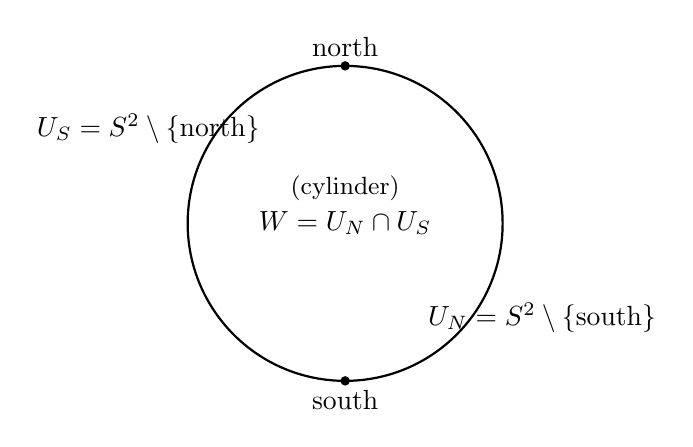
\begin{tikzpicture}[scale=2.0, line cap=round, line join=round]
		% sphere drawn as circle
		\draw[thick] (0,0) circle (1);
		% poles
		\fill (0,1) circle (0.03) node[above] {north};
		\fill (0,-1) circle (0.03) node[below] {south};
		
		% labels
		\node at (-1.25, 0.6) {$U_S=S^2\setminus\{\text{north}\}$};
		\node at ( 1.25,-0.6) {$U_N=S^2\setminus\{\text{south}\}$};
		\node at (0,0) {$W=U_N\cap U_S$};
		\node at (0,0.22) {\small(cylinder)};
	\end{tikzpicture}
\end{center}

\subsection*{(B) MV computation of $H^*(S^2)$}
Contractibility of $U_N,U_S$ gives
\[
H^1(U_N)=H^1(U_S)=0,\qquad H^2(U_N)=H^2(U_S)=0.
\]
Since $W\simeq S^1\times(0,1)$, we have
\[
H^1(W)\cong \R,\qquad H^2(W)=0.
\]
The key MV segment is
\[
H^1(U_N)\oplus H^1(U_S)\to H^1(W)\xrightarrow{\delta} H^2(S^2)\to H^2(U_N)\oplus H^2(U_S),
\]
which collapses to
\[
0\to \R \xrightarrow{\delta} H^2(S^2)\to 0,
\]
hence
\[
H^0(S^2)\cong \R,\qquad H^1(S^2)=0,\qquad H^2(S^2)\cong \R.
\]

\subsection*{(C) Generator via area form and Stokes (div/curl-type) obstruction}
In spherical coordinates $(\vartheta,\varphi)$ on $W$,
\[
\Omega := \sin\vartheta\, d\vartheta\wedge d\varphi
\]
is the standard area form on $S^2$, and
\[
\int_{S^2}\Omega = 4\pi \neq 0,
\]
so $\Omega$ is not exact (if $\Omega=dA$ globally then $\int_{S^2}\Omega=\int_{S^2}dA=0$ by Stokes).

Moreover, on the two charts one has explicit local potentials
\[
A_N=(1-\cos\vartheta)\,d\varphi\ \text{ on }U_N,\qquad
A_S=-(1+\cos\vartheta)\,d\varphi\ \text{ on }U_S,
\]
satisfying $dA_N=dA_S=\Omega$. On the overlap,
\[
A_N-A_S=2\,d\varphi,
\]
and $[d\varphi]$ generates $H^1(W)\cong \R$. The connecting map sends
\[
\delta\big([2\,d\varphi]\big)=[\Omega]\in H^2(S^2).
\]

\begin{center}
	\begin{tikzcd}[column sep=large]
		0 \arrow[r] &
		H^1(W) \arrow[r,"\delta","\cong"'] &
		H^2(S^2) \arrow[r] & 0
	\end{tikzcd}
\end{center}

\newpage
\section*{3. The torus $T^2=\R^2/\Z^2$ (complex torus)}

\subsection*{(A) Global closed forms, periods, and the expected answer}
The forms $dx,dy$ descend to $T^2$ and are closed.
For the fundamental loops $\gamma_x(t)=(t,0)$ and $\gamma_y(t)=(0,t)$ (mod $\Z^2$),
\[
\int_{\gamma_x} dx = 1,\quad \int_{\gamma_y} dx = 0,\qquad
\int_{\gamma_x} dy = 0,\quad \int_{\gamma_y} dy = 1.
\]
Hence $[dx],[dy]\neq 0$ in $H^1(T^2)$ (exact 1-forms have zero periods on loops).
Also $dx\wedge dy$ is closed and
\[
\int_{T^2} dx\wedge dy = 1\neq 0,
\]
so $[dx\wedge dy]\neq 0$ in $H^2(T^2)$.
Thus one expects
\[
H^0(T^2)\cong \R,\qquad H^1(T^2)\cong \R^2\langle[dx],[dy]\rangle,\qquad H^2(T^2)\cong \R\langle[dx\wedge dy]\rangle.
\]

\subsection*{(B) MV cover that recovers these classes}
Let
\[
C_0=\{x\equiv 0 \ (\mathrm{mod}\ 1)\},\qquad C_{1/2}=\{x\equiv \tfrac12 \ (\mathrm{mod}\ 1)\},
\]
and define
\[
U:=T^2\setminus C_0,\qquad V:=T^2\setminus C_{1/2}.
\]
Then $U\simeq S^1$, $V\simeq S^1$, and $U\cap V$ is a disjoint union of two cylinders
$A\sqcup B$ (two vertical open strips in the fundamental square).

\begin{center}
	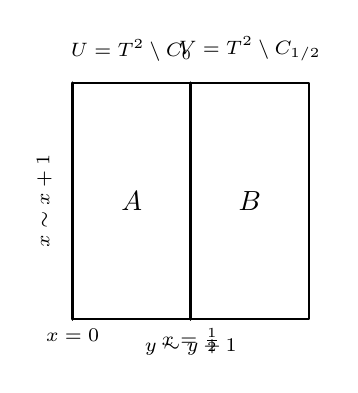
\begin{tikzpicture}[scale=3.0, line cap=round, line join=round]
		% fundamental domain
		\draw[thick] (0,0) rectangle (1,1);
		% identifications
		\node at (0.5,-0.12) {\scriptsize $y\sim y+1$};
		\node[rotate=90] at (-0.12,0.5) {\scriptsize $x\sim x+1$};
		
		% removed circles: x=0 and x=1/2
		\draw[very thick] (0,0) -- (0,1);
		\draw[very thick] (0.5,0) -- (0.5,1);
		\node[below] at (0,0) {\scriptsize $x=0$};
		\node[below] at (0.5,0) {\scriptsize $x=\tfrac12$};
		
		% overlap components A and B (schematic)
		\node at (0.25,0.5) {$A$};
		\node at (0.75,0.5) {$B$};
		
		% labels U and V
		\node[above] at (0.25,1.05) {\scriptsize $U=T^2\setminus C_0$};
		\node[above] at (0.75,1.05) {\scriptsize $V=T^2\setminus C_{1/2}$};
	\end{tikzpicture}
\end{center}

\subsection*{(C) MV segments (what they do)}
Cohomology of pieces:
\[
H^0(U)\cong H^0(V)\cong \R,\qquad H^1(U)\cong H^1(V)\cong \R,
\]
\[
H^0(U\cap V)\cong \R\oplus\R,\qquad H^1(U\cap V)\cong \R\oplus\R,\qquad H^2(U)=H^2(V)=H^2(U\cap V)=0.
\]

\paragraph{Degree 1: producing $[dx]$ and $[dy]$.}
The MV segment
\[
H^0(U\cap V)\xrightarrow{\delta} H^1(T^2)\to H^1(U)\oplus H^1(V)\to H^1(U\cap V)
\]
shows:
\begin{itemize}
	\item $\delta$ injects a copy of $\R$ (quotient of $H^0(U\cap V)$ by the diagonal) into $H^1(T^2)$; concretely it produces $[dx]$ from the ``difference of constants'' on the two components $A,B$.
	\item The kernel of $H^1(U)\oplus H^1(V)\to H^1(U\cap V)$ contributes the second independent class, represented globally by $[dy]$.
\end{itemize}
Hence $H^1(T^2)\cong \R^2$.

\paragraph{Degree 2: producing $[dx\wedge dy]$.}
The MV segment
\[
H^1(U\cap V)\xrightarrow{\delta} H^2(T^2)\to 0
\]
shows $H^2(T^2)$ is a quotient of $H^1(U\cap V)\cong \R^2$, killing the diagonal; the resulting $1$-dimensional quotient maps onto $H^2(T^2)$, and the nonzero integral
\[
\int_{T^2} dx\wedge dy = 1
\]
identifies the generator as $[dx\wedge dy]$ (up to sign).

\begin{center}
	\begin{tikzcd}[column sep=large]
		H^0(U\cap V) \arrow[r,"\delta"] &
		H^1(T^2) \arrow[r] &
		H^1(U)\oplus H^1(V) \arrow[r] &
		H^1(U\cap V)
	\end{tikzcd}
\end{center}

\begin{center}
	\begin{tikzcd}[column sep=large]
		H^1(U\cap V) \arrow[r,"\delta"] & H^2(T^2) \arrow[r] & 0
	\end{tikzcd}
\end{center}

\bigskip
\hrule
\bigskip

\section*{Quick reference: generators and ``potential'' obstructions}
\begin{itemize}
	\item $S^1$: generator $[d\theta]\in H^1(S^1)$ detected by $\int_{S^1} d\theta=2\pi$ (FTLI obstruction to being a global gradient).
	\item $S^2$: generator $[\Omega]\in H^2(S^2)$ detected by $\int_{S^2}\Omega=4\pi$ (Stokes obstruction to being $dA$ globally).
	\item $T^2$: generators $[dx],[dy]\in H^1(T^2)$ detected by loop periods; generator $[dx\wedge dy]\in H^2(T^2)$ detected by $\int_{T^2}dx\wedge dy=1$.
\end{itemize}






\chapter{Mayer–Vietoris Sequence and de Rham Cohomology}
Choose $\set[1]{V^k}_{k=0}^3$ and isomorphisms $\Phi^k:V^k\to\Omega^k(U)$ such that \[
\Phi^{k+1}\circ d^k=d\circ\Phi^k
\] where $d^0=\nabla$, $d^1=\nabla\times$, $d^2=\nabla\cdot$, and $d$ is exterior derivative.

\newpage
\section{Why the spaces $V^0,V^1,V^2,V^3$ are chosen as scalar and vector fields}

\subsection{Axiomatic goal}

\begin{definition}[Design requirement: transport of the de Rham differential]
	Let $U\subseteq \R^{3}$ be open and $\kk\in\{\R,\C\}$.
	Let $(V^\bullet,d_V)$ be a cochain complex of $\kk$-vector spaces concentrated in degrees $0,1,2,3$,
	i.e.\ $V^n=0$ for $n\notin\{0,1,2,3\}$.
	We say that $(V^\bullet,d_V)$ \emph{models the de Rham complex on $U$ via identifications}
	if there exist $\kk$-linear isomorphisms
	\[
	\Phi^{k}:V^{k}\xrightarrow{\cong}\Omega^{k}(U)\qquad(k=0,1,2,3)
	\]
	such that for all $k\in\{0,1,2\}$ the following diagram commutes:
	\[
	\begin{tikzcd}[column sep=large,row sep=large]
		V^{k} \arrow[r,"d_V^{k}"] \arrow[d,"\Phi^{k}"',"\cong"] &
		V^{k+1} \arrow[d,"\Phi^{k+1}"',"\cong"]\\
		\Omega^{k}(U) \arrow[r,"d"] &
		\Omega^{k+1}(U).
	\end{tikzcd}
	\]
	Equivalently,
	\[
	\Phi^{k+1}\circ d_V^{k}=d\circ \Phi^{k}\qquad(k=0,1,2).
	\]
\end{definition}

\subsection{Canonical identifications in Euclidean $\R^{3}$}

\begin{definition}[Scalar fields]
	Define
	\[
	V^{0}:=C^\infty(U;\kk),\qquad V^{3}:=C^\infty(U;\kk).
	\]
\end{definition}

\begin{remark}
	By definition of differential forms, $\Omega^{0}(U)=C^\infty(U;\kk)$.
	Moreover, fixing the standard orientation with volume form
	\[
	\mathrm{vol}:=dx_1\wedge dx_2\wedge dx_3,
	\]
	every $3$-form is uniquely of the form $h\,\mathrm{vol}$ with $h\in C^\infty(U;\kk)$, hence
	\[
	\Omega^{3}(U)\cong C^\infty(U;\kk)
	\]
	via $h\mapsto h\,\mathrm{vol}$.
\end{remark}

\begin{definition}[Vector fields and the Euclidean musical isomorphism]
	Define the $\kk$-vector space of (smooth) vector fields
	\[
	\mathfrak{X}(U;\kk):=C^\infty(U;\kk^{3}).
	\]
	Endow $U$ with the standard Euclidean metric $g=\sum_{i=1}^{3} dx_i\otimes dx_i$.
	Define the $\kk$-linear isomorphism
	\[
	\flat:\mathfrak{X}(U;\kk)\xrightarrow{\cong}\Omega^{1}(U)
	\]
	by the coordinate formula
	\[
	(P,Q,R)^\flat:=P\,dx_1+Q\,dx_2+R\,dx_3.
	\]
	Define
	\[
	V^{1}:=\mathfrak{X}(U;\kk)=C^\infty(U;\kk^{3}).
	\]
\end{definition}

\begin{definition}[Hodge star and the identification $\Omega^{2}\cong \mathfrak{X}$]
	With the Euclidean metric and orientation, let
	\[
	*:\Omega^{k}(U)\to\Omega^{3-k}(U)
	\]
	be the Hodge star.
	Define the $\kk$-linear isomorphism
	\[
	\Psi:\mathfrak{X}(U;\kk)\xrightarrow{\cong}\Omega^{2}(U),
	\qquad
	\Psi(G):=*(G^\flat).
	\]
	In coordinates, for $G=(A,B,C)$ one has
	\[
	\Psi(A,B,C)=A\,dx_2\wedge dx_3+B\,dx_3\wedge dx_1+C\,dx_1\wedge dx_2.
	\]
	Define
	\[
	V^{2}:=\mathfrak{X}(U;\kk)=C^\infty(U;\kk^{3}).
	\]
\end{definition}

\subsection{Compatibility with grad, curl, div}

\begin{definition}[The grad--curl--div differentials]
	Define $\kk$-linear maps
	\[
	\nabla:V^{0}\to V^{1},\qquad
	\nabla\times:V^{1}\to V^{2},\qquad
	\nabla\cdot:V^{2}\to V^{3}
	\]
	by the standard coordinate formulas
	\[
	\nabla f=(\partial_1 f,\partial_2 f,\partial_3 f),
	\]
	\[
	\nabla\times(P,Q,R)=(\partial_2 R-\partial_3 Q,\ \partial_3 P-\partial_1 R,\ \partial_1 Q-\partial_2 P),
	\]
	\[
	\nabla\cdot(A,B,C)=\partial_1 A+\partial_2 B+\partial_3 C.
	\]
\end{definition}

\begin{proposition}[Commuting transport and forced shapes of $V^k$]
	Let $\Phi^{0},\Phi^{1},\Phi^{2},\Phi^{3}$ be defined by
	\[
	\Phi^{0}=\id_{C^\infty(U;\kk)},\qquad
	\Phi^{1}=\flat,\qquad
	\Phi^{2}=\Psi,\qquad
	\Phi^{3}(h)=h\,\mathrm{vol}.
	\]
	Then
	\[
	\Phi^{1}\circ\nabla=d\circ\Phi^{0},\qquad
	\Phi^{2}\circ(\nabla\times)=d\circ\Phi^{1},\qquad
	\Phi^{3}\circ(\nabla\cdot)=d\circ\Phi^{2}.
	\]
	Consequently, the grad--curl--div complex
	\[
	0\to V^{0}\xrightarrow{\nabla}V^{1}\xrightarrow{\nabla\times}V^{2}\xrightarrow{\nabla\cdot}V^{3}\to 0
	\]
	is (via $\Phi^\bullet$) a transported model of the de Rham complex
	\[
	0\to\Omega^{0}(U)\xrightarrow{d}\Omega^{1}(U)\xrightarrow{d}\Omega^{2}(U)\xrightarrow{d}\Omega^{3}(U)\to 0.
	\]
\end{proposition}

\begin{proof}
	The equalities are verified by direct coordinate computation.
	Explicitly, for $f\in C^\infty(U;\kk)$,
	\[
	d(f)=\sum_{i=1}^{3}\partial_i f\,dx_i = (\nabla f)^\flat = \Phi^{1}(\nabla f).
	\]
	For $F=(P,Q,R)\in V^{1}$ one computes
	\[
	d(F^\flat)
	=(\partial_2 R-\partial_3 Q)\,dx_2\wedge dx_3
	+(\partial_3 P-\partial_1 R)\,dx_3\wedge dx_1
	+(\partial_1 Q-\partial_2 P)\,dx_1\wedge dx_2
	=\Psi(\nabla\times F)=\Phi^{2}(\nabla\times F),
	\]
	and for $G=(A,B,C)\in V^{2}$ one computes
	\[
	d(\Psi(G))=(\partial_1A+\partial_2B+\partial_3C)\,dx_1\wedge dx_2\wedge dx_3
	=(\nabla\cdot G)\,\mathrm{vol}=\Phi^{3}(\nabla\cdot G).
	\]
\end{proof}

\subsection{Uniqueness up to constant changes of basis}

\begin{theorem}[Uniqueness up to $\GL_{3}(\kk)$ in degrees $1$ and $2$]
	Let $\widetilde{\Phi}^{0},\widetilde{\Phi}^{1},\widetilde{\Phi}^{2},\widetilde{\Phi}^{3}$ be any linear isomorphisms
	\[
	\widetilde{\Phi}^{k}:V^{k}\xrightarrow{\cong}\Omega^{k}(U)\qquad(k=0,1,2,3)
	\]
	such that
	\[
	\widetilde{\Phi}^{1}\circ\nabla=d\circ\widetilde{\Phi}^{0},\qquad
	\widetilde{\Phi}^{2}\circ(\nabla\times)=d\circ\widetilde{\Phi}^{1},\qquad
	\widetilde{\Phi}^{3}\circ(\nabla\cdot)=d\circ\widetilde{\Phi}^{2},
	\]
	and assume $\widetilde{\Phi}^{0}=\id$ and $\widetilde{\Phi}^{3}(h)=h\,\mathrm{vol}$.
	Then there exists a constant matrix $A\in \GL_{3}(\kk)$ such that, after identifying
	$V^{1}=V^{2}=C^\infty(U;\kk^{3})$, one has
	\[
	\widetilde{\Phi}^{1}=\flat\circ A,\qquad \widetilde{\Phi}^{2}=\Psi\circ A,
	\]
	where $A$ acts pointwise on $C^\infty(U;\kk^{3})$ by $(AF)(x)=A(F(x))$.
\end{theorem}

\begin{proof}
	Define linear automorphisms $T^{1}:=\flat^{-1}\circ\widetilde{\Phi}^{1}$ and $T^{2}:=\Psi^{-1}\circ\widetilde{\Phi}^{2}$
	of $C^\infty(U;\kk^{3})$.
	The relations $\widetilde{\Phi}^{1}\circ\nabla=d\circ\id=\flat\circ\nabla$ and
	$\widetilde{\Phi}^{2}\circ(\nabla\times)=d\circ\widetilde{\Phi}^{1}=\Psi\circ(\nabla\times)\circ T^{1}$
	imply
	\[
	T^{1}\circ\nabla=\nabla,\qquad T^{2}\circ(\nabla\times)=(\nabla\times)\circ T^{1}.
	\]
	A standard linear-algebra/analysis argument shows that any $\kk$-linear endomorphism of
	$C^\infty(U;\kk^{3})$ commuting with all partial derivatives must be given by pointwise multiplication by
	a constant matrix in $\GL_{3}(\kk)$; denote this matrix by $A$.
	Then $T^{1}=A$ and the second commutation forces $T^{2}=A$ as well.
	Hence $\widetilde{\Phi}^{1}=\flat\circ A$ and $\widetilde{\Phi}^{2}=\Psi\circ A$.
\end{proof}

\begin{remark}
	The theorem formalizes the statement that, once one fixes the canonical identifications in degrees $0$ and $3$,
	the identifications in degrees $1$ and $2$ are unique up to an invertible constant change of basis of $\kk^{3}$.
\end{remark}

\newpage
\section{The grad--curl--div cochain complex and its cohomology}

\subsection{Vector spaces and linear maps}

\begin{definition}[Spaces of smooth fields]
	Let $U\subseteq \R^{3}$ be an open set and fix a field $\kk\in\{\R,\C\}$.
	Define $\kk$-vector spaces
	\[
	V^{0}:=C^\infty(U;\kk),\qquad
	V^{1}:=C^\infty(U;\kk^{3}),\qquad
	V^{2}:=C^\infty(U;\kk^{3}),\qquad
	V^{3}:=C^\infty(U;\kk),
	\]
	with pointwise addition and scalar multiplication.
	For all $n\in\Z\setminus\{0,1,2,3\}$ set $V^{n}:=0$.
\end{definition}

\begin{definition}[Differentials: $\nabla$, $\nabla\times$, $\nabla\cdot$]
	Write $(x_1,x_2,x_3)$ for the standard coordinates on $\R^{3}$ and $\partial_i:=\frac{\partial}{\partial x_i}$.
	Define $\kk$-linear maps
	\[
	d^{0}:V^{0}\to V^{1},\qquad d^{1}:V^{1}\to V^{2},\qquad d^{2}:V^{2}\to V^{3}
	\]
	by the following formulas:
	\begin{align*}
		d^{0}(f) &:= \nabla f := (\partial_{1}f,\partial_{2}f,\partial_{3}f),\\
		d^{1}(P,Q,R) &:= \nabla\times(P,Q,R) :=
		\bigl(\partial_{2}R-\partial_{3}Q,\ \partial_{3}P-\partial_{1}R,\ \partial_{1}Q-\partial_{2}P\bigr),\\
		d^{2}(A,B,C) &:= \nabla\cdot(A,B,C) := \partial_{1}A+\partial_{2}B+\partial_{3}C.
	\end{align*}
	For all $n\in\Z\setminus\{0,1,2\}$ define $d^{n}:V^{n}\to V^{n+1}$ to be the zero map.
\end{definition}

\begin{proposition}[The grad--curl--div complex]
	The sequence
	\[
	0\longrightarrow V^{0}\xrightarrow{\,d^{0}=\nabla\,} V^{1}\xrightarrow{\,d^{1}=\nabla\times\,} V^{2}
	\xrightarrow{\,d^{2}=\nabla\cdot\,} V^{3}\longrightarrow 0
	\]
	is a cochain complex, i.e.\ $d^{1}\circ d^{0}=0$ and $d^{2}\circ d^{1}=0$.
	Equivalently,
	\[
	\nabla\times(\nabla f)=0\quad \forall f\in C^\infty(U;\kk),
	\qquad
	\nabla\cdot(\nabla\times F)=0\quad \forall F\in C^\infty(U;\kk^3).
	\]
\end{proposition}

\begin{proof}
	Let $f\in C^\infty(U;\kk)$. Then
	\[
	(\nabla\times \nabla f)_1
	=\partial_{2}(\partial_{3}f)-\partial_{3}(\partial_{2}f)=0
	\]
	by commutativity of mixed partials; similarly $(\nabla\times\nabla f)_2=(\nabla\times\nabla f)_3=0$.
	Hence $d^{1}d^{0}=0$.
	
	Let $F=(P,Q,R)\in C^\infty(U;\kk^3)$. Then
	\begin{align*}
		\nabla\cdot(\nabla\times F)
		&=\partial_1(\partial_2R-\partial_3Q)+\partial_2(\partial_3P-\partial_1R)+\partial_3(\partial_1Q-\partial_2P)\\
		&=\partial_1\partial_2R-\partial_1\partial_3Q+\partial_2\partial_3P-\partial_2\partial_1R+\partial_3\partial_1Q-\partial_3\partial_2P\\
		&=0
	\end{align*}
	again by commutativity of mixed partial derivatives and cancellation. Thus $d^{2}d^{1}=0$.
\end{proof}

\subsection{Cohomology and interpretation}

\begin{definition}[Cocycles, coboundaries, cohomology]
	Let $(V^\bullet,d)$ be the grad--curl--div cochain complex above.
	For each $n\in\Z$ define
	\[
	Z^{n}:=\ker(d^{n})\subseteq V^{n},\qquad
	B^{n}:=\im(d^{n-1})\subseteq V^{n},
	\qquad
	H^{n}(V^\bullet):=Z^{n}/B^{n}.
	\]
\end{definition}

\begin{proposition}[Cohomology groups of the grad--curl--div complex]
	With the conventions $d^{-1}=0$ and $d^{3}=0$ one has:
	\begin{align*}
		H^{0}(V^\bullet)
		&\cong \ker(\nabla)=\{f\in C^\infty(U;\kk):\nabla f=0\},\\[4pt]
		H^{1}(V^\bullet)
		&\cong \ker(\nabla\times)/\im(\nabla)
		=\dfrac{\{F\in C^\infty(U;\kk^3):\nabla\times F=0\}}{\{\nabla f:f\in C^\infty(U;\kk)\}},\\[10pt]
		H^{2}(V^\bullet)
		&\cong \ker(\nabla\cdot)/\im(\nabla\times)
		=\dfrac{\{G\in C^\infty(U;\kk^3):\nabla\cdot G=0\}}{\{\nabla\times F:F\in C^\infty(U;\kk^3)\}},\\[10pt]
		H^{3}(V^\bullet)
		&\cong V^{3}/\im(\nabla\cdot)
		=\dfrac{C^\infty(U;\kk)}{\{\nabla\cdot G:G\in C^\infty(U;\kk^3)\}}.
	\end{align*}
\end{proposition}

\begin{remark}[Interpretation]
	$H^{1}$ measures curl-free vector fields modulo gradients (obstructions to global scalar potentials).
	$H^{2}$ measures divergence-free vector fields modulo curls (obstructions to global vector potentials).
	$H^{3}$ measures functions modulo divergences.
\end{remark}

\subsection{Identification with the de Rham complex (formal transport)}

\begin{definition}[de Rham complex]
	Let $\Omega^{k}(U)$ denote the $\kk$-vector space of smooth differential $k$-forms on $U$.
	The exterior derivative is a $\kk$-linear map
	\[
	d:\Omega^{k}(U)\to \Omega^{k+1}(U)
	\]
	satisfying $d\circ d=0$.
	The associated cohomology spaces are
	\[
	H^{k}_{\mathrm{dR}}(U):=\ker\bigl(d:\Omega^{k}(U)\to \Omega^{k+1}(U)\bigr)\Big/\im\bigl(d:\Omega^{k-1}(U)\to \Omega^{k}(U)\bigr).
	\]
\end{definition}

\begin{definition}[Musical isomorphism and Hodge star (Euclidean)]
	Equip $U\subseteq\R^{3}$ with the standard Euclidean metric and orientation.
	Let $\flat:C^\infty(U;\kk^3)\to\Omega^{1}(U)$ denote the metric identification (``lowering an index'').
	Let $*: \Omega^{k}(U)\to\Omega^{3-k}(U)$ denote the Hodge star operator.
\end{definition}

\begin{proposition}[Commuting diagram with de Rham]
	Define linear isomorphisms
	\[
	\Phi^{0}:V^{0}\xrightarrow{\cong}\Omega^{0}(U),\quad \Phi^{0}(f)=f,
	\]
	\[
	\Phi^{1}:V^{1}\xrightarrow{\cong}\Omega^{1}(U),\quad \Phi^{1}(F)=F^{\flat},
	\]
	\[
	\Phi^{2}:V^{2}\xrightarrow{\cong}\Omega^{2}(U),\quad \Phi^{2}(G)=*(G^{\flat}),
	\]
	\[
	\Phi^{3}:V^{3}\xrightarrow{\cong}\Omega^{3}(U),\quad \Phi^{3}(h)=h\,dx_{1}\wedge dx_{2}\wedge dx_{3}.
	\]
	Then the following diagram commutes:
	\[
	\begin{tikzcd}[column sep=large,row sep=large]
		0 \arrow[r] &
		V^{0} \arrow[r,"\nabla"] \arrow[d,"\Phi^{0}"',"\cong"] &
		V^{1} \arrow[r,"\nabla\times"] \arrow[d,"\Phi^{1}"',"\cong"] &
		V^{2} \arrow[r,"\nabla\cdot"] \arrow[d,"\Phi^{2}"',"\cong"] &
		V^{3} \arrow[r] \arrow[d,"\Phi^{3}"',"\cong"] &
		0\\
		0 \arrow[r] &
		\Omega^{0}(U) \arrow[r,"d"] &
		\Omega^{1}(U) \arrow[r,"d"] &
		\Omega^{2}(U) \arrow[r,"d"] &
		\Omega^{3}(U) \arrow[r] &
		0
	\end{tikzcd}
	\]
	Consequently, for each $k\in\{0,1,2,3\}$ there is an induced isomorphism
	\[
	H^{k}(V^\bullet)\cong H^{k}_{\mathrm{dR}}(U).
	\]
\end{proposition}

\begin{corollary}[Contractible case]
	If $U$ is contractible (e.g.\ $U$ is star-shaped), then
	\[
	H^{k}(V^\bullet)=0\ \text{for all }k\in\{1,2,3\},
	\]
	and if $U$ is connected then $H^{0}(V^\bullet)\cong \kk$.
\end{corollary}

\newpage
\section{The grad--curl--div cochain complex and its identification with the de Rham complex}

\subsection{The grad--curl--div cochain complex}

\begin{definition}[Spaces and differentials]
	Let $U\subseteq \R^{3}$ be open and fix $\kk\in\{\R,\C\}$.
	Define $\kk$-vector spaces
	\[
	V^{0}:=C^\infty(U;\kk),\quad
	V^{1}:=C^\infty(U;\kk^{3}),\quad
	V^{2}:=C^\infty(U;\kk^{3}),\quad
	V^{3}:=C^\infty(U;\kk).
	\]
	Write $(x_1,x_2,x_3)$ for the standard coordinates and $\partial_i:=\frac{\partial}{\partial x_i}$.
	Define $\kk$-linear maps
	\[
	d^{0}:V^{0}\to V^{1},\qquad d^{1}:V^{1}\to V^{2},\qquad d^{2}:V^{2}\to V^{3}
	\]
	by
	\begin{align*}
		d^{0}(f)&:=\nabla f:=(\partial_1 f,\partial_2 f,\partial_3 f),\\
		d^{1}(P,Q,R)&:=\nabla\times(P,Q,R):=
		(\partial_2 R-\partial_3 Q,\ \partial_3 P-\partial_1 R,\ \partial_1 Q-\partial_2 P),\\
		d^{2}(A,B,C)&:=\nabla\cdot(A,B,C):=\partial_1 A+\partial_2 B+\partial_3 C.
	\end{align*}
\end{definition}

\begin{proposition}[Cochain complex condition]
	One has $d^{1}\circ d^{0}=0$ and $d^{2}\circ d^{1}=0$. Hence
	\[
	0\longrightarrow V^{0}\xrightarrow{\ \nabla\ } V^{1}\xrightarrow{\ \nabla\times\ } V^{2}\xrightarrow{\ \nabla\cdot\ } V^{3}\longrightarrow 0
	\]
	is a cochain complex.
\end{proposition}

\begin{proof}
	This follows immediately from the computations
	\[
	\nabla\times(\nabla f)=0,\qquad \nabla\cdot(\nabla\times F)=0,
	\]
	which are verified componentwise using commutativity of mixed partial derivatives.
\end{proof}

\subsection{Cohomology of the grad--curl--div complex}

\begin{definition}[Cohomology]
	For each $n\in\{0,1,2,3\}$ define
	\[
	Z^{n}:=\Ker(d^{n})\subseteq V^{n},\qquad B^{n}:=\im(d^{n-1})\subseteq V^{n},
	\qquad H^{n}(V^\bullet):=Z^{n}/B^{n},
	\]
	with the conventions $d^{-1}=0$ and $d^{3}=0$.
\end{definition}

\begin{proposition}[Concrete description]
	One has canonical identifications
	\begin{align*}
		H^{0}(V^\bullet)
		&\cong \Ker(\nabla),\\[4pt]
		H^{1}(V^\bullet)
		&\cong \Ker(\nabla\times)\big/\im(\nabla),\\[6pt]
		H^{2}(V^\bullet)
		&\cong \Ker(\nabla\cdot)\big/\im(\nabla\times),\\[6pt]
		H^{3}(V^\bullet)
		&\cong V^{3}\big/\im(\nabla\cdot).
	\end{align*}
\end{proposition}

\subsection{Differential forms on \(U\subseteq\mathbb{R}^3\)}

\begin{definition}[de Rham complex]
	Let $\Omega^{k}(U)$ be the $\kk$-vector space of smooth $k$-forms on $U$.
	The exterior derivative is the $\kk$-linear map
	\[
	d:\Omega^{k}(U)\to\Omega^{k+1}(U)
	\]
	characterized in coordinates by the usual rules (graded Leibniz rule and $d(dx_i)=0$),
	and satisfies $d\circ d=0$.
	The $k$-th de Rham cohomology is
	\[
	H^{k}_{\mathrm{dR}}(U):=\Ker\bigl(d:\Omega^{k}(U)\to\Omega^{k+1}(U)\bigr)\Big/\im\bigl(d:\Omega^{k-1}(U)\to\Omega^{k}(U)\bigr).
	\]
\end{definition}

\subsection{Explicit formulas for \(\flat\) and \(*\)}

\begin{definition}[Euclidean musical isomorphisms]
	Endow $U\subseteq\R^3$ with the standard Euclidean metric
	$g=\sum_{i=1}^{3} dx_i\otimes dx_i$.
	Define the $\kk$-linear map (``lowering an index'')
	\[
	\flat: C^\infty(U;\kk^3)\to \Omega^{1}(U)
	\]
	by the coordinate formula
	\[
	(P,Q,R)^\flat := P\,dx_1 + Q\,dx_2 + R\,dx_3.
	\]
	Its inverse $\sharp:\Omega^{1}(U)\to C^\infty(U;\kk^3)$ is given by
	\[
	(a_1 dx_1+a_2 dx_2+a_3 dx_3)^\sharp := (a_1,a_2,a_3).
	\]
\end{definition}

\begin{definition}[Hodge star in \(\R^3\)]
	Fix the standard orientation, with volume form
	\[
	\mathrm{vol}:=dx_1\wedge dx_2\wedge dx_3\in\Omega^{3}(U).
	\]
	Define the Hodge star operator $*:\Omega^{k}(U)\to\Omega^{3-k}(U)$ by specifying its values on the standard basis:
	\begin{align*}
		*&1=\mathrm{vol},\\
		&*dx_1=dx_2\wedge dx_3,\quad *dx_2=dx_3\wedge dx_1,\quad *dx_3=dx_1\wedge dx_2,\\
		&*(dx_2\wedge dx_3)=dx_1,\quad *(dx_3\wedge dx_1)=dx_2,\quad *(dx_1\wedge dx_2)=dx_3,\\
		&*\mathrm{vol}=1,
	\end{align*}
	and extending \(\kk\)-linearly.
\end{definition}

\subsection{Transport of the de Rham differential to grad--curl--div}

\begin{definition}[The comparison isomorphisms \(\Phi^k\)]
	Define \(\kk\)-linear isomorphisms
	\[
	\Phi^{0}:V^{0}\xrightarrow{\cong}\Omega^{0}(U),\quad \Phi^{0}(f):=f,
	\]
	\[
	\Phi^{1}:V^{1}\xrightarrow{\cong}\Omega^{1}(U),\quad \Phi^{1}(F):=F^\flat,
	\]
	\[
	\Phi^{2}:V^{2}\xrightarrow{\cong}\Omega^{2}(U),\quad \Phi^{2}(G):=*(G^\flat),
	\]
	\[
	\Phi^{3}:V^{3}\xrightarrow{\cong}\Omega^{3}(U),\quad \Phi^{3}(h):=h\,\mathrm{vol}.
	\]
\end{definition}

\begin{proposition}[Commutativity of the comparison diagram]
	For all $f\in V^{0}$, $F\in V^{1}$, $G\in V^{2}$, one has
	\[
	\Phi^{1}(\nabla f)=d(\Phi^{0}(f)),\qquad
	\Phi^{2}(\nabla\times F)=d(\Phi^{1}(F)),\qquad
	\Phi^{3}(\nabla\cdot G)=d(\Phi^{2}(G)).
	\]
	Equivalently, the diagram of cochain complexes commutes:
	\[
	\begin{tikzcd}[column sep=large,row sep=large]
		0 \arrow[r] &
		V^{0} \arrow[r,"\nabla"] \arrow[d,"\Phi^{0}"',"\cong"] &
		V^{1} \arrow[r,"\nabla\times"] \arrow[d,"\Phi^{1}"',"\cong"] &
		V^{2} \arrow[r,"\nabla\cdot"] \arrow[d,"\Phi^{2}"',"\cong"] &
		V^{3} \arrow[r] \arrow[d,"\Phi^{3}"',"\cong"] &
		0\\
		0 \arrow[r] &
		\Omega^{0}(U) \arrow[r,"d"] &
		\Omega^{1}(U) \arrow[r,"d"] &
		\Omega^{2}(U) \arrow[r,"d"] &
		\Omega^{3}(U) \arrow[r] &
		0.
	\end{tikzcd}
	\]
\end{proposition}

\begin{proof}
	\emph{Step 1: grad.}
	Let $f\in V^{0}=C^\infty(U;\kk)$. Then
	\[
	d(\Phi^{0}(f))=d(f)=\partial_1 f\,dx_1+\partial_2 f\,dx_2+\partial_3 f\,dx_3
	=(\nabla f)^\flat=\Phi^{1}(\nabla f).
	\]
	
	\emph{Step 2: curl.}
	Let $F=(P,Q,R)\in V^{1}$. Then $\Phi^{1}(F)=F^\flat=P\,dx_1+Q\,dx_2+R\,dx_3$, hence
	\begin{align*}
		d(\Phi^{1}(F))
		&=d(P)\wedge dx_1+d(Q)\wedge dx_2+d(R)\wedge dx_3\\
		&=(\partial_1 P\,dx_1+\partial_2 P\,dx_2+\partial_3 P\,dx_3)\wedge dx_1\\
		&\qquad+(\partial_1 Q\,dx_1+\partial_2 Q\,dx_2+\partial_3 Q\,dx_3)\wedge dx_2\\
		&\qquad+(\partial_1 R\,dx_1+\partial_2 R\,dx_2+\partial_3 R\,dx_3)\wedge dx_3.
	\end{align*}
	Using $dx_i\wedge dx_i=0$ and $dx_j\wedge dx_i=-dx_i\wedge dx_j$, this simplifies to
	\begin{align*}
		d(\Phi^{1}(F))
		&=(\partial_2 P)\,dx_2\wedge dx_1+(\partial_3 P)\,dx_3\wedge dx_1\\
		&\quad+(\partial_1 Q)\,dx_1\wedge dx_2+(\partial_3 Q)\,dx_3\wedge dx_2\\
		&\quad+(\partial_1 R)\,dx_1\wedge dx_3+(\partial_2 R)\,dx_2\wedge dx_3\\
		&=(\partial_2 R-\partial_3 Q)\,dx_2\wedge dx_3
		+(\partial_3 P-\partial_1 R)\,dx_3\wedge dx_1
		+(\partial_1 Q-\partial_2 P)\,dx_1\wedge dx_2.
	\end{align*}
	On the other hand,
	\[
	\nabla\times F=
	(\partial_2 R-\partial_3 Q,\ \partial_3 P-\partial_1 R,\ \partial_1 Q-\partial_2 P),
	\]
	so
	\begin{align*}
		\Phi^{2}(\nabla\times F)
		&=*((\nabla\times F)^\flat)\\
		&=*(\,(\partial_2 R-\partial_3 Q)\,dx_1+(\partial_3 P-\partial_1 R)\,dx_2+(\partial_1 Q-\partial_2 P)\,dx_3\,)\\
		&=(\partial_2 R-\partial_3 Q)\,dx_2\wedge dx_3
		+(\partial_3 P-\partial_1 R)\,dx_3\wedge dx_1
		+(\partial_1 Q-\partial_2 P)\,dx_1\wedge dx_2.
	\end{align*}
	Comparing, $d(\Phi^{1}(F))=\Phi^{2}(\nabla\times F)$.
	
	\emph{Step 3: div.}
	Let $G=(A,B,C)\in V^{2}$. Then
	\[
	\Phi^{2}(G)=*(G^\flat)=*(A\,dx_1+B\,dx_2+C\,dx_3)
	=A\,dx_2\wedge dx_3+B\,dx_3\wedge dx_1+C\,dx_1\wedge dx_2.
	\]
	Therefore
	\begin{align*}
		d(\Phi^{2}(G))
		&=d(A)\wedge dx_2\wedge dx_3+d(B)\wedge dx_3\wedge dx_1+d(C)\wedge dx_1\wedge dx_2\\
		&=(\partial_1 A\,dx_1+\partial_2 A\,dx_2+\partial_3 A\,dx_3)\wedge dx_2\wedge dx_3\\
		&\quad+(\partial_1 B\,dx_1+\partial_2 B\,dx_2+\partial_3 B\,dx_3)\wedge dx_3\wedge dx_1\\
		&\quad+(\partial_1 C\,dx_1+\partial_2 C\,dx_2+\partial_3 C\,dx_3)\wedge dx_1\wedge dx_2\\
		&=(\partial_1 A)\,dx_1\wedge dx_2\wedge dx_3
		+(\partial_2 B)\,dx_2\wedge dx_3\wedge dx_1
		+(\partial_3 C)\,dx_3\wedge dx_1\wedge dx_2\\
		&=(\partial_1 A+\partial_2 B+\partial_3 C)\,dx_1\wedge dx_2\wedge dx_3\\
		&=(\nabla\cdot G)\,\mathrm{vol}
		=\Phi^{3}(\nabla\cdot G).
	\end{align*}
	This completes the proof.
\end{proof}

\begin{corollary}[Cohomology identification]
	The maps $\Phi^{k}$ induce isomorphisms on cohomology:
	\[
	H^{k}(V^\bullet)\cong H^{k}_{\mathrm{dR}}(U)\qquad (k=0,1,2,3).
	\]
\end{corollary}

\begin{remark}[Topology and ``potential'' obstructions]
	Under the identification above, $H^{1}(V^\bullet)$ measures curl-free fields modulo gradients, and
	$H^{2}(V^\bullet)$ measures divergence-free fields modulo curls.
	If $U$ is contractible (e.g.\ star-shaped), then $H^{k}_{\mathrm{dR}}(U)=0$ for $k\ge 1$, hence
	$H^{1}(V^\bullet)=H^{2}(V^\bullet)=H^{3}(V^\bullet)=0$.
\end{remark}

\newpage
\section{Cochain complexes and grad--curl--div as de Rham cohomology in $\R^{3}$}

\subsection{Formal construction of differential forms on an open set of $\R^{3}$}

\begin{definition}[Coordinate ring of smooth functions]
	Let $U\subseteq \R^{3}$ be open. For a field $\kk\in\{\R,\C\}$ define
	\[
	\Omega^{0}(U):=C^\infty(U;\kk),
	\]
	viewed as a commutative unital $\kk$-algebra under pointwise operations.
\end{definition}

\begin{definition}[The $\kk$-vector spaces $\Omega^{1}(U),\Omega^{2}(U),\Omega^{3}(U)$]
	Let $(x_1,x_2,x_3)$ be the standard coordinate functions on $U$.
	Define $\Omega^{1}(U)$ to be the free $\Omega^{0}(U)$-module with basis $\{dx_1,dx_2,dx_3\}$, i.e.
	\[
	\Omega^{1}(U):=\Omega^{0}(U)\,dx_1 \oplus \Omega^{0}(U)\,dx_2 \oplus \Omega^{0}(U)\,dx_3.
	\]
	Define $\Omega^{2}(U)$ to be the free $\Omega^{0}(U)$-module with basis
	$\{dx_1\wedge dx_2,\ dx_2\wedge dx_3,\ dx_3\wedge dx_1\}$, i.e.
	\[
	\Omega^{2}(U):=\Omega^{0}(U)\,(dx_1\wedge dx_2)\oplus
	\Omega^{0}(U)\,(dx_2\wedge dx_3)\oplus
	\Omega^{0}(U)\,(dx_3\wedge dx_1).
	\]
	Define $\Omega^{3}(U)$ to be the free $\Omega^{0}(U)$-module of rank $1$ with basis
	\[
	\mathrm{vol}:=dx_1\wedge dx_2\wedge dx_3,
	\qquad
	\Omega^{3}(U):=\Omega^{0}(U)\,\mathrm{vol}.
	\]
\end{definition}

\begin{definition}[Wedge product on coordinate forms]
	Define a $\kk$-bilinear map
	\[
	\wedge:\Omega^{p}(U)\times \Omega^{q}(U)\to \Omega^{p+q}(U)
	\]
	by imposing the following axioms:
	\begin{enumerate}
		\item $\wedge$ is $\Omega^{0}(U)$-bilinear in the sense that for $f\in\Omega^{0}(U)$ and forms $\alpha,\beta$
		\[
		(f\alpha)\wedge\beta=f(\alpha\wedge\beta),\qquad \alpha\wedge(f\beta)=f(\alpha\wedge\beta);
		\]
		\item $\wedge$ is associative;
		\item on basis elements it is alternating:
		\[
		dx_i\wedge dx_i=0,\qquad dx_i\wedge dx_j=-\,dx_j\wedge dx_i\quad(i\neq j);
		\]
		\item $1\in\Omega^{0}(U)$ acts as a unit: $1\wedge\alpha=\alpha=\alpha\wedge 1$ for all $\alpha$.
	\end{enumerate}
\end{definition}

\begin{remark}[Coordinate expansions]
	Every $\alpha\in\Omega^{1}(U)$ has a unique expression
	\[
	\alpha=a_1\,dx_1+a_2\,dx_2+a_3\,dx_3\qquad(a_i\in\Omega^{0}(U)),
	\]
	every $\beta\in\Omega^{2}(U)$ has a unique expression
	\[
	\beta=b_{12}\,dx_1\wedge dx_2+b_{23}\,dx_2\wedge dx_3+b_{31}\,dx_3\wedge dx_1
	\qquad(b_{ij}\in\Omega^{0}(U)),
	\]
	and every $\gamma\in\Omega^{3}(U)$ has a unique expression $\gamma=c\,\mathrm{vol}$ with $c\in\Omega^{0}(U)$.
\end{remark}

\subsection{Formal definition of the exterior derivative}

\begin{definition}[Exterior derivative in coordinates]
	Define $\kk$-linear maps
	\[
	d:\Omega^{k}(U)\to\Omega^{k+1}(U)\qquad(k=0,1,2)
	\]
	by the following coordinate rules.
	\begin{enumerate}
		\item If $f\in\Omega^{0}(U)$, define
		\[
		df:=\partial_1 f\,dx_1+\partial_2 f\,dx_2+\partial_3 f\,dx_3\in\Omega^{1}(U).
		\]
		\item If $\alpha=a_1dx_1+a_2dx_2+a_3dx_3\in\Omega^{1}(U)$, define
		\begin{align*}
			d\alpha
			&:=da_1\wedge dx_1+da_2\wedge dx_2+da_3\wedge dx_3\\
			&=(\partial_2 a_1-\partial_1 a_2)\,dx_1\wedge dx_2
			+(\partial_3 a_2-\partial_2 a_3)\,dx_2\wedge dx_3
			+(\partial_1 a_3-\partial_3 a_1)\,dx_3\wedge dx_1
			\in\Omega^{2}(U).
		\end{align*}
		\item If $\beta=b_{12}dx_1\wedge dx_2+b_{23}dx_2\wedge dx_3+b_{31}dx_3\wedge dx_1\in\Omega^{2}(U)$, define
		\begin{align*}
			d\beta
			&:=db_{12}\wedge dx_1\wedge dx_2+db_{23}\wedge dx_2\wedge dx_3+db_{31}\wedge dx_3\wedge dx_1\\
			&=(\partial_3 b_{12}+\partial_1 b_{23}+\partial_2 b_{31})\,dx_1\wedge dx_2\wedge dx_3
			\in\Omega^{3}(U).
		\end{align*}
	\end{enumerate}
	Finally define $d:\Omega^{3}(U)\to 0$ to be the zero map.
\end{definition}

\begin{proposition}[Graded Leibniz rule]
	For all $p,q\ge 0$ with $p+q\le 3$, and all $\alpha\in\Omega^{p}(U)$, $\beta\in\Omega^{q}(U)$, one has
	\[
	d(\alpha\wedge\beta)=d\alpha\wedge\beta+(-1)^{p}\alpha\wedge d\beta.
	\]
\end{proposition}

\begin{proposition}[$d^2=0$]
	The maps $d:\Omega^{k}(U)\to\Omega^{k+1}(U)$ satisfy $d\circ d=0$, i.e.
	\[
	d^{2}=0:\Omega^{k}(U)\to\Omega^{k+2}(U)\qquad\text{for }k=0,1,2.
	\]
\end{proposition}

\begin{proof}
	It suffices to check $d(df)=0$ for $f\in\Omega^{0}(U)$ and $d(d\alpha)=0$ for $\alpha\in\Omega^{1}(U)$.
	The coordinate formulas show each coefficient is a sum of mixed second derivatives which cancel by
	$\partial_i\partial_j=\partial_j\partial_i$.
\end{proof}

\begin{definition}[de Rham cochain complex and cohomology]
	The sequence
	\[
	0\to \Omega^{0}(U)\xrightarrow{d}\Omega^{1}(U)\xrightarrow{d}\Omega^{2}(U)\xrightarrow{d}\Omega^{3}(U)\to 0
	\]
	is a cochain complex. Its cohomology vector spaces are
	\[
	H^{k}_{\mathrm{dR}}(U):=\Ker\bigl(d:\Omega^{k}(U)\to\Omega^{k+1}(U)\bigr)\Big/\im\bigl(d:\Omega^{k-1}(U)\to\Omega^{k}(U)\bigr).
	\]
\end{definition}

\subsection{grad, curl, div as transported differentials}

\begin{definition}[Vector-field spaces and vector-calculus differentials]
	Let $V^{0}:=C^\infty(U;\kk)$, $V^{1}:=C^\infty(U;\kk^{3})$, $V^{2}:=C^\infty(U;\kk^{3})$, $V^{3}:=C^\infty(U;\kk)$.
	Define
	\[
	\nabla:V^{0}\to V^{1},\qquad \nabla\times:V^{1}\to V^{2},\qquad \nabla\cdot:V^{2}\to V^{3}
	\]
	by
	\begin{align*}
		\nabla f&:=(\partial_1 f,\partial_2 f,\partial_3 f),\\
		\nabla\times(P,Q,R)&:=(\partial_2 R-\partial_3 Q,\ \partial_3 P-\partial_1 R,\ \partial_1 Q-\partial_2 P),\\
		\nabla\cdot(A,B,C)&:=\partial_1A+\partial_2B+\partial_3C.
	\end{align*}
\end{definition}

\begin{definition}[Explicit identifications $\Phi^k$]
	Equip $U$ with the Euclidean metric and standard orientation.
	Define linear isomorphisms
	\[
	\Phi^{0}:V^{0}\xrightarrow{\cong}\Omega^{0}(U),\quad \Phi^{0}(f)=f,
	\]
	\[
	\Phi^{1}:V^{1}\xrightarrow{\cong}\Omega^{1}(U),\quad \Phi^{1}(P,Q,R)=P\,dx_1+Q\,dx_2+R\,dx_3,
	\]
	\[
	\Phi^{2}:V^{2}\xrightarrow{\cong}\Omega^{2}(U),\quad \Phi^{2}(A,B,C)=A\,dx_2\wedge dx_3+B\,dx_3\wedge dx_1+C\,dx_1\wedge dx_2,
	\]
	\[
	\Phi^{3}:V^{3}\xrightarrow{\cong}\Omega^{3}(U),\quad \Phi^{3}(h)=h\,dx_1\wedge dx_2\wedge dx_3.
	\]
\end{definition}

\begin{proposition}[Diagram commutativity: explicit proof]
	For all $f\in V^{0}$, $F\in V^{1}$, $G\in V^{2}$,
	\[
	\Phi^{1}(\nabla f)=d(\Phi^{0}(f)),\qquad
	\Phi^{2}(\nabla\times F)=d(\Phi^{1}(F)),\qquad
	\Phi^{3}(\nabla\cdot G)=d(\Phi^{2}(G)).
	\]
	Equivalently, the following diagram commutes:
	\[
	\begin{tikzcd}[column sep=large,row sep=large]
		0 \arrow[r] &
		V^{0} \arrow[r,"\nabla"] \arrow[d,"\Phi^{0}"',"\cong"] &
		V^{1} \arrow[r,"\nabla\times"] \arrow[d,"\Phi^{1}"',"\cong"] &
		V^{2} \arrow[r,"\nabla\cdot"] \arrow[d,"\Phi^{2}"',"\cong"] &
		V^{3} \arrow[r] \arrow[d,"\Phi^{3}"',"\cong"] &
		0\\
		0 \arrow[r] &
		\Omega^{0}(U) \arrow[r,"d"] &
		\Omega^{1}(U) \arrow[r,"d"] &
		\Omega^{2}(U) \arrow[r,"d"] &
		\Omega^{3}(U) \arrow[r] &
		0.
	\end{tikzcd}
	\]
\end{proposition}

\begin{proof}
	\emph{(i) grad.}
	For $f\in V^{0}$,
	\[
	d(\Phi^{0}(f))=df=\partial_1 f\,dx_1+\partial_2 f\,dx_2+\partial_3 f\,dx_3=\Phi^{1}(\nabla f).
	\]
	
	\emph{(ii) curl.}
	Let $F=(P,Q,R)\in V^{1}$. Then $\Phi^{1}(F)=Pdx_1+Qdx_2+Rdx_3$. Hence
	\begin{align*}
		d(\Phi^{1}(F))
		&=d(P)\wedge dx_1+d(Q)\wedge dx_2+d(R)\wedge dx_3\\
		&=(\partial_2R-\partial_3Q)\,dx_2\wedge dx_3
		+(\partial_3P-\partial_1R)\,dx_3\wedge dx_1
		+(\partial_1Q-\partial_2P)\,dx_1\wedge dx_2.
	\end{align*}
	By definition,
	\[
	\nabla\times F=(\partial_2R-\partial_3Q,\ \partial_3P-\partial_1R,\ \partial_1Q-\partial_2P),
	\]
	so
	\[
	\Phi^{2}(\nabla\times F)
	=(\partial_2R-\partial_3Q)\,dx_2\wedge dx_3
	+(\partial_3P-\partial_1R)\,dx_3\wedge dx_1
	+(\partial_1Q-\partial_2P)\,dx_1\wedge dx_2.
	\]
	Thus $d(\Phi^{1}(F))=\Phi^{2}(\nabla\times F)$.
	
	\emph{(iii) div.}
	Let $G=(A,B,C)\in V^{2}$. Then
	\[
	\Phi^{2}(G)=A\,dx_2\wedge dx_3+B\,dx_3\wedge dx_1+C\,dx_1\wedge dx_2.
	\]
	Hence
	\begin{align*}
		d(\Phi^{2}(G))
		&=d(A)\wedge dx_2\wedge dx_3+d(B)\wedge dx_3\wedge dx_1+d(C)\wedge dx_1\wedge dx_2\\
		&=(\partial_1A+\partial_2B+\partial_3C)\,dx_1\wedge dx_2\wedge dx_3
		=\Phi^{3}(\nabla\cdot G).
	\end{align*}
\end{proof}

\subsection{Cohomology on the vector-calculus side}

\begin{definition}[Cohomology of grad--curl--div]
	Define $d^{0}:=\nabla$, $d^{1}:=\nabla\times$, $d^{2}:=\nabla\cdot$, and extend by $d^{-1}=0$, $d^{3}=0$.
	Define
	\[
	Z^{n}:=\Ker(d^{n}),\qquad B^{n}:=\im(d^{n-1}),\qquad H^{n}(V^\bullet):=Z^{n}/B^{n}
	\quad (n=0,1,2,3).
	\]
	Equivalently,
	\begin{align*}
		H^{0}(V^\bullet)&=\Ker(\nabla),\\
		H^{1}(V^\bullet)&=\Ker(\nabla\times)\big/\im(\nabla),\\
		H^{2}(V^\bullet)&=\Ker(\nabla\cdot)\big/\im(\nabla\times),\\
		H^{3}(V^\bullet)&=C^\infty(U;\kk)\big/\im(\nabla\cdot).
	\end{align*}
\end{definition}

\begin{corollary}[Identification with de Rham cohomology]
	For each $k\in\{0,1,2,3\}$, the isomorphisms $\Phi^{k}$ induce canonical isomorphisms
	\[
	H^{k}(V^\bullet)\cong H^{k}_{\mathrm{dR}}(U).
	\]
\end{corollary}

\begin{remark}[Contractible domains]
	If $U$ is contractible, then $H^{k}_{\mathrm{dR}}(U)=0$ for $k\ge 1$ and (if $U$ is connected) $H^{0}_{\mathrm{dR}}(U)\cong \kk$.
	Consequently $H^{1}(V^\bullet)=H^{2}(V^\bullet)=H^{3}(V^\bullet)=0$ and $H^{0}(V^\bullet)\cong\kk$.
\end{remark}



\newpage
\section{Cochain complexes of vector spaces}

\begin{definition}[Graded vector space]
	Fix a field $\kk$.
	A \emph{$\Z$-graded $\kk$-vector space} is a family $V^\bullet=\{V^n\}_{n\in\Z}$ of $\kk$-vector spaces.
\end{definition}

\begin{definition}[Cochain complex]
	A \emph{cochain complex of $\kk$-vector spaces} is a pair $(V^\bullet,d)$ where
	\begin{enumerate}
		\item $V^\bullet=\{V^n\}_{n\in\Z}$ is a $\Z$-graded $\kk$-vector space;
		\item $d=\{d^n\}_{n\in\Z}$ is a family of $\kk$-linear maps
		\[
		d^n:V^n\longrightarrow V^{n+1}\qquad(n\in\Z)
		\]
		such that
		\[
		d^{n+1}\circ d^n = 0\qquad\text{for all }n\in\Z.
		\]
	\end{enumerate}
	In diagrammatic form, one writes
	\[
	\cdots \xrightarrow{d^{n-2}} V^{n-1}\xrightarrow{d^{n-1}} V^n\xrightarrow{d^n}V^{n+1}\xrightarrow{d^{n+1}}\cdots,
	\qquad d^n d^{n-1}=0.
	\]
\end{definition}

\begin{remark}[The condition $d^{n+1}d^n=0$]
	For each $n\in\Z$ the equality $d^{n+1}\circ d^n=0$ is an equality of $\kk$-linear maps
	$V^n\to V^{n+2}$. Equivalently,
	\[
	\forall v\in V^n,\quad d^{n+1}\bigl(d^n(v)\bigr)=0.
	\]
\end{remark}

\section{Cocycles, coboundaries, and cohomology}

\begin{definition}[Cocycles and coboundaries]
	Let $(V^\bullet,d)$ be a cochain complex.
	For each $n\in\Z$ define the subspaces
	\[
	Z^n(V^\bullet):=\ker(d^n)\subseteq V^n,
	\qquad
	B^n(V^\bullet):=\im(d^{n-1})\subseteq V^n.
	\]
	Elements of $Z^n(V^\bullet)$ are called \emph{$n$-cocycles}, and elements of
	$B^n(V^\bullet)$ are called \emph{$n$-coboundaries}.
\end{definition}

\begin{lemma}[Coboundaries are cocycles]
	For every $n\in\Z$ one has $B^n(V^\bullet)\subseteq Z^n(V^\bullet)$.
\end{lemma}

\begin{proof}
	Let $x\in B^n(V^\bullet)$. By definition, $\exists\,y\in V^{n-1}$ such that $x=d^{n-1}(y)$.
	Then
	\[
	d^n(x)=d^n\!\bigl(d^{n-1}(y)\bigr)=\bigl(d^n\circ d^{n-1}\bigr)(y)=0,
	\]
	hence $x\in\ker(d^n)=Z^n(V^\bullet)$.
\end{proof}

\begin{definition}[Cohomology]
	Let $(V^\bullet,d)$ be a cochain complex.
	For each $n\in\Z$ the \emph{$n$-th cohomology vector space} is the quotient
	\[
	H^n(V^\bullet):=Z^n(V^\bullet)\big/ B^n(V^\bullet)
	=\ker(d^n)\big/\im(d^{n-1}).
	\]
\end{definition}

\begin{remark}[Cohomology classes and equivalence relation]
	Fix $n\in\Z$. Define a binary relation $\sim$ on $Z^n(V^\bullet)$ by
	\[
	z\sim z' \;\;\Longleftrightarrow\;\; z-z'\in B^n(V^\bullet).
	\]
	Then $\sim$ is an equivalence relation on $Z^n(V^\bullet)$ (reflexive, symmetric, transitive),
	and the quotient set $Z^n(V^\bullet)/{\sim}$ inherits a unique $\kk$-vector space structure
	for which the canonical projection $Z^n(V^\bullet)\to Z^n(V^\bullet)/{\sim}$ is $\kk$-linear.
	Under this identification one has
	\[
	Z^n(V^\bullet)/{\sim}\;\cong\; Z^n(V^\bullet)\big/ B^n(V^\bullet)=H^n(V^\bullet).
	\]
\end{remark}

\section{Functoriality}

\begin{definition}[Morphism of cochain complexes]
	Let $(V^\bullet,d_V)$ and $(W^\bullet,d_W)$ be cochain complexes of $\kk$-vector spaces.
	A \emph{morphism of cochain complexes} (or \emph{cochain map})
	$f:(V^\bullet,d_V)\to(W^\bullet,d_W)$ is a family of $\kk$-linear maps
	\[
	f^n:V^n\to W^n\qquad(n\in\Z)
	\]
	such that
	\[
	d_W^n\circ f^n = f^{n+1}\circ d_V^n\qquad\text{for all }n\in\Z.
	\]
\end{definition}

\begin{proposition}[Induced map on cohomology]
	Let $f:(V^\bullet,d_V)\to(W^\bullet,d_W)$ be a cochain map.
	For each $n\in\Z$ there exists a unique $\kk$-linear map
	\[
	H^n(f):H^n(V^\bullet)\to H^n(W^\bullet)
	\]
	such that for every $z\in Z^n(V^\bullet)$ one has
	\[
	H^n(f)\bigl([z]\bigr)=[f^n(z)].
	\]
\end{proposition}

\begin{proof}
	First, if $z\in Z^n(V^\bullet)$ then
	\[
	d_W^n\bigl(f^n(z)\bigr)= (d_W^n\circ f^n)(z)=(f^{n+1}\circ d_V^n)(z)=f^{n+1}(0)=0,
	\]
	so $f^n(z)\in Z^n(W^\bullet)$ and $[f^n(z)]$ is defined.
	
	To check well-definedness on cohomology classes: if $[z]=[z']$ in $H^n(V^\bullet)$ then
	$z-z'\in B^n(V^\bullet)$, so $\exists\,y\in V^{n-1}$ with $z-z'=d_V^{n-1}(y)$.
	Hence
	\[
	f^n(z)-f^n(z')=f^n(z-z')=f^n\!\bigl(d_V^{n-1}(y)\bigr)
	=(f^n\circ d_V^{n-1})(y)=(d_W^{n-1}\circ f^{n-1})(y)\in \im(d_W^{n-1})=B^n(W^\bullet).
	\]
	Thus $[f^n(z)]=[f^n(z')]$ in $H^n(W^\bullet)$, so the formula defines a function
	$H^n(f)$.
	
	Linearity follows because the quotient map $Z^n(V^\bullet)\to H^n(V^\bullet)$ is linear
	and $f^n$ is linear. Uniqueness holds because every class in $H^n(V^\bullet)$ has a cocycle representative.
\end{proof}

\section{Finite-dimensional dimension formula}

\begin{proposition}[Dimension identity]
	Assume each $V^n$ is finite-dimensional. Then for all $n\in\Z$,
	\[
	\dim_\kk H^n(V^\bullet)=\dim_\kk \ker(d^n) - \dim_\kk \im(d^{n-1})
	= \nullity(d^n)-\rank(d^{n-1}).
	\]
\end{proposition}

\begin{proof}
	Since $B^n(V^\bullet)\subseteq Z^n(V^\bullet)$, the quotient $H^n(V^\bullet)=Z^n/B^n$
	is a vector space and
	\[
	\dim_\kk H^n(V^\bullet)=\dim_\kk Z^n(V^\bullet)-\dim_\kk B^n(V^\bullet).
	\]
	By definition $Z^n=\ker(d^n)$ and $B^n=\im(d^{n-1})$, giving the stated formula.
\end{proof}

\begin{example}[Two-step complex]
	Let $V^0,V^1,V^2$ be $\kk$-vector spaces and let $d^0:V^0\to V^1$, $d^1:V^1\to V^2$ be linear maps
	satisfying $d^1d^0=0$. Extend by $V^n=0$ for $n\notin\{0,1,2\}$ and $d^n=0$ otherwise.
	Then
	\[
	H^0 \cong \ker(d^0),\qquad
	H^1 \cong \ker(d^1)/\im(d^0),\qquad
	H^2 \cong V^2/\im(d^1),
	\]
	and $H^n=0$ for $n\notin\{0,1,2\}$.
\end{example}


\newpage
\begin{definition}[Graded object]
	Let $\mathcal{A}$ be an abelian category. A \emph{$\Z$-graded object} of $\mathcal{A}$ is a family
	$A^\bullet = \{A^k\}_{k\in\Z}$ of objects of $\mathcal{A}$.
\end{definition}

\begin{definition}[Cochain complex]
	A \emph{cochain complex} in $\mathcal{A}$ is a pair $(A^\bullet,d)$ consisting of a $\Z$-graded object
	$A^\bullet$ and morphisms
	\[
	d^k : A^k \longrightarrow A^{k+1} \qquad (k\in\Z)
	\]
	such that
	\[
	d^{k+1}\circ d^k = 0 \qquad \text{for all } k\in\Z.
	\]
	We write the complex as
	\[
	\cdots \xrightarrow{d^{k-2}} A^{k-1}\xrightarrow{d^{k-1}} A^k\xrightarrow{d^k} A^{k+1}\xrightarrow{d^{k+1}} \cdots .
	\]
\end{definition}

\begin{definition}[Morphisms of cochain complexes]
	Let $(A^\bullet,d_A)$ and $(B^\bullet,d_B)$ be cochain complexes in $\mathcal{A}$.
	A \emph{morphism of complexes} (or \emph{cochain map})
	$f:(A^\bullet,d_A)\to(B^\bullet,d_B)$ is a family of morphisms
	\[
	f^k: A^k \to B^k \qquad (k\in\Z)
	\]
	such that
	\[
	d_B^k\circ f^k = f^{k+1}\circ d_A^k \qquad \text{for all }k\in\Z.
	\]
\end{definition}

\section{Cocycles, coboundaries, and cohomology}

\begin{definition}[Cocycles and coboundaries]
	Let $(A^\bullet,d)$ be a cochain complex in an abelian category $\mathcal{A}$.
	Define
	\[
	Z^k(A^\bullet) := \ker(d^k)\subseteq A^k,
	\qquad
	B^k(A^\bullet) := \im(d^{k-1})\subseteq A^k.
	\]
\end{definition}

\begin{lemma}[Boundaries are cycles]
	For every $k\in\Z$ one has $B^k(A^\bullet)\subseteq Z^k(A^\bullet)$.
\end{lemma}

\begin{proof}
	Let $x\in B^k(A^\bullet)$. Then $x=d^{k-1}(y)$ for some $y\in A^{k-1}$, hence
	\[
	d^k(x)=d^k(d^{k-1}(y))=(d^k\circ d^{k-1})(y)=0
	\]
	by the defining condition $d^k\circ d^{k-1}=0$. Therefore $x\in\ker(d^k)=Z^k(A^\bullet)$.
\end{proof}

\begin{definition}[Cohomology]
	The \emph{$k$-th cohomology object} of $(A^\bullet,d)$ is
	\[
	H^k(A^\bullet) := Z^k(A^\bullet)\big/ B^k(A^\bullet)
	= \ker(d^k)\big/\im(d^{k-1}).
	\]
\end{definition}

\begin{remark}[Cohomology classes]
	If $\mathcal{A}=\Ab$ (or $R$-$\Mod$), elements of $H^k(A^\bullet)$ are classes $[\alpha]$ with
	$\alpha\in Z^k(A^\bullet)$, and $[\alpha]=[\alpha']$ iff $\alpha-\alpha' \in B^k(A^\bullet)$, i.e.\ iff
	$\alpha-\alpha' = d^{k-1}\beta$ for some $\beta\in A^{k-1}$.
\end{remark}

\section{Exactness}

\begin{definition}[Exactness]
	A cochain complex $(A^\bullet,d)$ is \emph{exact at $A^k$} if
	\[
	\im(d^{k-1}) = \ker(d^k).
	\]
	It is \emph{exact} if it is exact at every degree.
\end{definition}

\begin{proposition}[Exactness and vanishing cohomology]
	A cochain complex $(A^\bullet,d)$ is exact if and only if $H^k(A^\bullet)=0$ for all $k\in\Z$.
\end{proposition}

\begin{proof}
	By definition,
	\[
	H^k(A^\bullet)=0 \iff \ker(d^k)=\im(d^{k-1}).
	\]
	Thus vanishing of all cohomology objects is equivalent to exactness in every degree.
\end{proof}

\section{Homotopy of cochain maps}

\begin{definition}[Cochain homotopy]
	Let $f,g:(A^\bullet,d_A)\to(B^\bullet,d_B)$ be cochain maps.
	A \emph{cochain homotopy} from $f$ to $g$ is a family of morphisms
	\[
	h^k: A^k \to B^{k-1} \qquad (k\in\Z)
	\]
	such that
	\[
	f^k-g^k = d_B^{k-1}\circ h^k + h^{k+1}\circ d_A^k
	\qquad\text{for all }k\in\Z.
	\]
	We write $f\simeq g$ if there exists such a homotopy.
\end{definition}

\begin{proposition}[Homotopic maps induce the same map on cohomology]
	If $f\simeq g$, then $H^k(f)=H^k(g)$ for all $k\in\Z$.
\end{proposition}

\begin{proof}
	Let $\alpha\in Z^k(A^\bullet)$, so $d_A^k(\alpha)=0$. Then
	\[
	(f^k-g^k)(\alpha)=d_B^{k-1}(h^k(\alpha)) + h^{k+1}(d_A^k(\alpha))
	= d_B^{k-1}(h^k(\alpha)),
	\]
	so $f^k(\alpha)-g^k(\alpha)\in \im(d_B^{k-1})=B^k(B^\bullet)$.
	Hence $[f^k(\alpha)]=[g^k(\alpha)]$ in $H^k(B^\bullet)$.
\end{proof}

\section{Mapping cone and long exact sequence}

\begin{definition}[Shift]
	Given a complex $(A^\bullet,d_A)$, its \emph{shift} $A[1]^\bullet$ is defined by
	\[
	A[1]^k := A^{k+1}, \qquad d_{A[1]}^k := -\,d_A^{k+1}.
	\]
\end{definition}

\begin{definition}[Mapping cone]
	Let $f:(A^\bullet,d_A)\to(B^\bullet,d_B)$ be a cochain map.
	The \emph{mapping cone} $\mathrm{Cone}(f)$ is the complex with
	\[
	\mathrm{Cone}(f)^k := B^k \oplus A^{k+1}
	\]
	and differential
	\[
	d_{\mathrm{Cone}(f)}^k(b,a) := \bigl(d_B^k(b) + f^{k+1}(a),\, -d_A^{k+1}(a)\bigr).
	\]
\end{definition}

\begin{lemma}
	$\mathrm{Cone}(f)$ is a cochain complex, i.e.\ $d_{\mathrm{Cone}(f)}^{k+1}\circ d_{\mathrm{Cone}(f)}^k=0$.
\end{lemma}

\begin{proof}
	A direct computation using $d_B\circ d_B=0$, $d_A\circ d_A=0$, and $d_B\circ f=f\circ d_A$.
\end{proof}

\begin{proposition}[Short exact sequence of complexes]
	There is a natural short exact sequence of complexes
	\[
	0 \longrightarrow B^\bullet \xrightarrow{i} \mathrm{Cone}(f)^\bullet \xrightarrow{p} A[1]^\bullet \longrightarrow 0,
	\]
	where $i(b)=(b,0)$ and $p(b,a)=a$ in each degree.
\end{proposition}

\begin{theorem}[Long exact sequence in cohomology]
	Let $0\to X^\bullet \to Y^\bullet \to Z^\bullet \to 0$ be a short exact sequence of cochain complexes in an abelian category.
	Then there exist connecting morphisms $\delta^k:H^k(Z^\bullet)\to H^{k+1}(X^\bullet)$ such that
	\[
	\cdots \to H^k(X^\bullet)\to H^k(Y^\bullet)\to H^k(Z^\bullet)\xrightarrow{\delta^k} H^{k+1}(X^\bullet)\to H^{k+1}(Y^\bullet)\to \cdots
	\]
	is exact.
\end{theorem}

\begin{remark}[Explicit connecting morphism in $\Ab$ or $R$-$\Mod$]
	Suppose $0\to X^\bullet \xrightarrow{u} Y^\bullet \xrightarrow{v} Z^\bullet\to 0$ is degreewise exact.
	Given $[z]\in H^k(Z^\bullet)$ with $z\in Z^k(Z^\bullet)$, choose $y\in Y^k$ with $v(y)=z$.
	Then $v(d_Y^k y)=d_Z^k(v(y))=d_Z^k(z)=0$, hence $d_Y^k y\in \ker(v)=\im(u)$.
	Choose $x\in X^{k+1}$ with $u(x)=d_Y^k y$ and set $\delta^k([z]) := [x]\in H^{k+1}(X^\bullet)$.
	One checks $\delta^k$ is well-defined and yields exactness.
\end{remark}

\section{Examples}

\begin{example}[de Rham complex]
	For a smooth manifold $M$, the graded $\mathbb{R}$-vector space $\Omega^\bullet(M)$ with exterior derivative
	$d:\Omega^k(M)\to\Omega^{k+1}(M)$ satisfies $d\circ d=0$, hence forms a cochain complex.
	Its cohomology is
	\[
	H^k_{\mathrm{dR}}(M) := \ker\bigl(d:\Omega^k(M)\to\Omega^{k+1}(M)\bigr)\Big/\im\bigl(d:\Omega^{k-1}(M)\to\Omega^k(M)\bigr).
	\]
\end{example}

\begin{example}[Singular cochains]
	Let $X$ be a topological space and $G\in\Ab$.
	Let $C_k(X)$ be the singular chain group and define $C^k(X;G):=\Hom(C_k(X),G)$.
	The coboundary $\delta:C^k(X;G)\to C^{k+1}(X;G)$ satisfies $\delta^2=0$.
	The cohomology $H^k(C^\bullet(X;G))$ is the singular cohomology $H^k(X;G)$.
\end{example}


\chapter{Elliptic Curve and Torus}
\section{Note 1: Meromorphic Function and Order}

\newpage
\section{Note 2: Meromorphic $f\in\C^X$ and Holomorphic $F\in(\CP^1)^X$}
Given a meromorphic $f:X\to\C$ on a Riemann surface $X$, we define \[
\fullfunction{F}{X}{\C\cup\set{\infty}(\simeq\CP^1)}{p}{F(p)=\begin{cases}
[1:f(p)] &\text{if $p$ is not a pole} \\
[0:1] &\text{if $p$ is a pole}
\end{cases}}
\]
\begin{figure}[h!]\centering
\includegraphics[scale=1]{tikzs/X_to_CP1}
\end{figure}

\medskip\noindent
In other word, \begin{figure}[h!]\centering
% https://q.uiver.app/#q=WzAsOCxbMCwwLCJYIl0sWzIsMCwiXFxtYXRoYmJ7Q30iXSxbNCwwLCJcXG1hdGhiYntDUH1eMSJdLFswLDEsInBfe1xcdGV4dHtub24tcG9sZX19Il0sWzAsMiwicV97XFx0ZXh0e3BvbGV9fSJdLFsyLDEsImYocCkiXSxbNCwxLCJbZihwKToxXSJdLFs0LDIsIlsxOjBdIl0sWzAsMSwiZiJdLFsxLDIsImkiXSxbMyw1LCIiLDAseyJzdHlsZSI6eyJ0YWlsIjp7Im5hbWUiOiJtYXBzIHRvIn19fV0sWzUsNiwiIiwwLHsic3R5bGUiOnsidGFpbCI6eyJuYW1lIjoibWFwcyB0byJ9fX1dLFs0LDcsIiIsMCx7InN0eWxlIjp7InRhaWwiOnsibmFtZSI6Im1hcHMgdG8ifX19XV0=
\[\begin{tikzcd}
	X && {\mathbb{C}} && {\mathbb{CP}^1} \\
	{p_{\text{non-pole}}} && {f(p)} && {[z_0\;\text{:}\;z_1]=[1\;\text{:}\;z_1/z_0]=[1\;\text{:}\;f(p)]} \\
	{q_{\text{pole}}} &&&& {[0\;\text{:}\;1]=\infty}
	\arrow["f", from=1-1, to=1-3]
	\arrow["i", from=1-3, to=1-5]
	\arrow[maps to, from=2-1, to=2-3]
	\arrow[maps to, from=2-3, to=2-5]
	\arrow[maps to, from=3-1, to=3-5]
\end{tikzcd}\]
\end{figure}

\newpage
% Examples: meromorphic f and holomorphic F:X->CP^1
\subsection{Example 1: \(X = \mathbb{CP}^1\) (Riemann sphere)}
We view \(\mathbb{CP}^1\) as the Riemann sphere. On the affine chart \[
U_1 = \{[z_0:z_1]\in\mathbb{CP}^1 \mid z_1\neq 0\},
\] we use the coordinate $z = {z_0}/{z_1}.$ The point at infinity is \(\infty = [1:0]\).

On \(\mathbb{CP}^1\), a meromorphic function is the same as a rational function.
Take for instance
\[
f(z) = \frac{z^2 - 1}{z - 2}.
\]
This is meromorphic on \(\mathbb{CP}^1\), with a simple pole at \(z=2\), and (possibly) a pole at \(\infty\).

Define
\[
F:\mathbb{CP}^1\to\mathbb{CP}^1,\qquad
F(p) =
\begin{cases}
	[f(p):1], & p \text{ not a pole of } f,\\[4pt]
	[1:0], & p \text{ a pole of } f.
\end{cases}
\]

Concretely, for \(p=[z:1]\) with \(z\neq 2\),
\[
F([z:1]) = [f(z):1] = \left[\dfrac{z^2-1}{z-2}:1\right],
\]
and at the pole \(p=[2:1]\),
\[
F([2:1]) = [1:0].
\]
Similarly one checks the value at \(\infty=[1:0]\) using the behavior of \(f(z)\) as
\(|z|\to\infty\).

To see that \(F\) is holomorphic, we use the usual charts on \(\mathbb{CP}^1\):

\begin{itemize}
	\item \textbf{At a non-pole point \(p\).} Suppose \(p\) is not a pole of \(f\).
	Then \(f\) is holomorphic near \(p\) and finite there, so \(F(p)=[f(p):1]\in U_1\).
	Let
	\[
	w = \frac{z_0}{z_1}:U_1\to\mathbb{C}
	\]
	be the affine coordinate on \(U_1\). In this chart,
	\[
	(w\circ F)(q) = \frac{z_0}{z_1}\Big|_{F(q)} = f(q),
	\]
	which is holomorphic in any local coordinate around \(p\). Hence \(F\) is holomorphic at non-poles.
	
	\item \textbf{At a pole \(p\).} Let \(p\) be a pole of order \(m>0\). Choose a local
	coordinate \(z\) on \(\mathbb{CP}^1\) with \(z(p)=0\). Then
	\[
	f(z) = z^{-m} g(z),\qquad g \text{ holomorphic, } g(0)\neq 0.
	\]
	Here \(F(p)=[1:0]\). Use the chart
	\[
	U_0 = \{[z_0:z_1]\in\mathbb{CP}^1 \mid z_0\neq 0\},
	\]
	with coordinate
	\[
	u = \frac{z_1}{z_0} : U_0\to\mathbb{C}.
	\]
	For \(z\neq 0\) near \(p\),
	\[
	F(z) = [f(z):1] = [z^{-m}g(z):1].
	\]
	Multiplying homogeneous coordinates by \(z^m\) (which does not change the point in
	projective space), we get
	\[
	[z^{-m}g(z):1] = [g(z):z^m].
	\]
	Thus, in the chart \(U_0\),
	\[
	(u\circ F)(z) = \frac{z^m}{g(z)}.
	\]
	Since \(g(z)\) is holomorphic with \(g(0)\neq 0\), the function
	\(\dfrac{1}{g(z)}\) is holomorphic near \(0\), and hence
	\[
	\frac{z^m}{g(z)}
	\]
	is holomorphic near \(0\) (and vanishes to order \(m\)). Therefore \(F\) is holomorphic at the pole \(p\).
\end{itemize}

Since we have holomorphicity in local charts at every point of \(\mathbb{CP}^1\),
\(F:\mathbb{CP}^1\to\mathbb{CP}^1\) is a holomorphic map.


\bigskip
\bigskip


\subsection{Example 2: \(X = \mathbb{C}/\Lambda\) (complex torus)}

Let \(\Lambda\subset\mathbb{C}\) be a lattice and consider the complex torus
\[
X = \mathbb{C}/\Lambda.
\]
The quotient map is
\[
\pi:\mathbb{C}\to X,\qquad \pi(z) = [z].
\]

A meromorphic function \(f:X\to\mathbb{C}\) corresponds to a \(\Lambda\)-periodic
meromorphic function \(\tilde f:\mathbb{C}\to\mathbb{C}\) satisfying
\[
\tilde f(z+\lambda) = \tilde f(z),\quad \forall\,\lambda\in\Lambda,
\]
and
\[
f([z]) = \tilde f(z).
\]

A standard example is the Weierstrass \(\wp\)-function \(\wp:\mathbb{C}\to\mathbb{C}\),
which is \(\Lambda\)-periodic and meromorphic with double poles at lattice points.
Thus it descends to a meromorphic
\[
f:X\to\mathbb{C},\qquad f([z]) = \wp(z).
\]

We define
\[
F:X\to\mathbb{CP}^1,\qquad
F(p) =
\begin{cases}
	[f(p):1], & p \text{ not a pole of } f,\\[4pt]
	[1:0], & p \text{ a pole of } f.
\end{cases}
\]

For our example \(f([z])=\wp(z)\):

\begin{itemize}
	\item \(\wp(z)\) has poles precisely at lattice points \(z\in\Lambda\),
	which all represent the same point on the torus, usually denoted \([0]\).
	\item For \([z]\neq[0]\), we set \(F([z]) = [\wp(z):1]\).
	\item At \([0]\), we set \(F([0]) = [1:0]\).
\end{itemize}

\subsubsection{Local coordinate on the torus near a pole}

To get a local coordinate near \([0]\in X\), choose a small disc
\(D\subset\mathbb{C}\) around \(0\) such that
\(\pi|_D:D\to \pi(D)\) is a biholomorphism.
Then
\[
\varphi:\pi(D)\to\mathbb{C},\qquad \varphi([z]) = z,
\]
is a local coordinate on \(X\) near \([0]\).

The local behavior of \(\wp(z)\) at \(z=0\) is
\[
\wp(z) = \frac{1}{z^2} + \text{holomorphic terms},
\]
so more precisely,
\[
\wp(z) = z^{-2} g(z),\qquad g(z)\ \text{holomorphic, } g(0)\neq 0.
\]
Thus, for the induced \(f\),
\[
f([z]) = \wp(z) = z^{-2} g(z),
\]
so \(f\) has a pole of order \(m=2\) at \([0]\).

\subsubsection{Holomorphicity of \(F\) at the pole \([0]\)}

As before, we use the chart around \([1:0]\in\mathbb{CP}^1\):
\[
U_0 = \{[z_0:z_1]\mid z_0\neq 0\},\qquad
u = \frac{z_1}{z_0}:U_0\to\mathbb{C}.
\]

For \(z\neq 0\) small, we have \(p=[z]\neq[0]\) and
\[
F([z]) = [f([z]):1] = [\wp(z):1] = [z^{-2}g(z):1].
\]
Multiplying the homogeneous coordinates by \(z^2\) gives
\[
[z^{-2}g(z):1] = [g(z):z^2].
\]
So in the chart \(U_0\),
\[
(u\circ F)([z]) = \frac{z^2}{g(z)}.
\]

Since \(g(z)\) is holomorphic with \(g(0)\neq 0\), the function
\(\dfrac{1}{g(z)}\) is holomorphic near \(0\), and hence \(\dfrac{z^2}{g(z)}\)
is holomorphic near \(0\) and vanishes at \(z=0\). In the local coordinate
\(\varphi([z])=z\) on \(X\), the expression
\[
u\circ F\circ \varphi^{-1}(z) = \frac{z^2}{g(z)}
\]
is holomorphic, so \(F\) is holomorphic at the pole \([0]\).

At a non-pole point \([z_0]\in X\), the same argument as in Example~1 applies:
\(f\) is holomorphic and finite, and in the affine chart
\[
U_1 = \{[z_0:z_1]\mid z_1\neq 0\},\qquad w = \frac{z_0}{z_1},
\]
we have
\[
(w\circ F)([z]) = f([z]) = \wp(z),
\]
which is holomorphic in the local coordinate on \(X\).

\subsubsection{Conclusion}

For both examples \(X=\mathbb{CP}^1\) and \(X=\mathbb{C}/\Lambda\), the construction
\[
f:X\to\mathbb{C}\ \text{meromorphic} \quad\longmapsto\quad
F:X\to\mathbb{CP}^1,\quad
F(p)=
\begin{cases}
	[f(p):1], & p \text{ not a pole},\\[4pt]
	[1:0], & p \text{ a pole},
\end{cases}
\]
produces a holomorphic map \(F:X\to\mathbb{CP}^1\). This concretely illustrates
the general principle that a meromorphic function on a Riemann surface is the same
as a holomorphic map to \(\mathbb{CP}^1\).


\newpage
We start with a meromorphic function
\[
f:X\to\mathbb{C}
\]
on a Riemann surface \(X\), and define a map
\[
F:X\to\mathbb{CP}^1
\]
by
\[
F(p)=
\begin{cases}
	[f(p):1], & p \text{ not a pole of } f,\\[4pt]
	[1:0], & p \text{ a pole of } f.
\end{cases}
\]

You’re asking: \textbf{why is this \(F\) holomorphic as a map of Riemann surfaces?}

\bigskip

%-----------------------------------------
\section*{1. Definition to remember}

A map \(F:X\to Y\) between Riemann surfaces is \textbf{holomorphic} if, for every point
\(p\in X\), you can choose local coordinates
\begin{itemize}
	\item \(\varphi\): neighborhood of \(p\to \mathbb{C}\),
	\item \(\psi\): neighborhood of \(F(p)\to \mathbb{C}\),
\end{itemize}
such that the coordinate expression
\[
\psi \circ F \circ \varphi^{-1} : \text{(open in }\mathbb{C})\to \mathbb{C}
\]
is an ordinary holomorphic function.

So we need to check this around:
\begin{enumerate}
	\item a point where \(f\) is holomorphic (no pole),
	\item a point where \(f\) has a pole.
\end{enumerate}

\bigskip

%-----------------------------------------
\section*{2. Case 1: \(p\) is \textbf{not} a pole (easy)}

If \(p\) is not a pole, then \(f\) is holomorphic near \(p\) and finite there.

\begin{itemize}
	\item On \(X\): choose any local coordinate \(z\) with \(z(p)=0\).
	\item On \(\mathbb{CP}^1\): since \(F(p)=[f(p):1]\) has second coordinate \(\neq 0\),
	it lies in the chart
	\[
	U_1 = \{[z_0:z_1]\mid z_1\neq 0\}
	\]
	with coordinate
	\[
	w = \frac{z_0}{z_1} : U_1\to\mathbb{C}.
	\]
\end{itemize}

Then on some neighborhood of \(p\),
\[
(w\circ F)(q) = \frac{z_0}{z_1}\Big|_{F(q)}
= \frac{f(q)}{1}
= f(q),
\]
which is holomorphic in \(z\).

So \(\psi\circ F\circ\varphi^{-1} = f\) is holomorphic \(\Rightarrow F\) is holomorphic at non-pole points.

\bigskip

%-----------------------------------------
\section*{3. Case 2: \(p\) is a \textbf{pole} of order \(m>0\)}

This is the interesting part.

Let \(p\) be a pole of \(f\) of order \(m\). Choose a local coordinate \(z\) on \(X\)
with \(z(p)=0\). By the definition of meromorphic:
\[
f(z) = z^{-m} g(z),
\]
where \(g\) is holomorphic and \(g(0)\neq 0\).

By definition,
\[
F(p) = [1:0] \in \mathbb{CP}^1.
\]

Now we must look at a chart of \(\mathbb{CP}^1\) that contains \([1:0]\). That is:
\[
U_0 = \{[z_0:z_1]\mid z_0\neq 0\},
\]
with coordinate
\[
u = \frac{z_1}{z_0} : U_0\to\mathbb{C},
\]
and in this chart \([1:0]\) corresponds to \(u=0\).

For \(z \neq 0\) near \(p\),
\[
F(z) = [f(z):1] = [z^{-m}g(z):1].
\]

Multiply homogeneous coordinates by \(z^m\) (allowed in projective space):
\[
[z^{-m}g(z):1] = [g(z):z^m].
\]

So in the chart \(U_0\) we have:
\[
u(F(z)) = \frac{z^m}{g(z)}.
\]

Now, check holomorphicity:
\begin{itemize}
	\item \(g(z)\) is holomorphic with \(g(0)\neq 0\) \(\Rightarrow 1/g(z)\) is holomorphic near \(0\).
	\item \(z^m\) is holomorphic.
	\item The product \(z^m \cdot \dfrac{1}{g(z)}\) is holomorphic near \(0\).
\end{itemize}

So
\[
u\circ F(z) = \frac{z^m}{g(z)}
\]
is an ordinary holomorphic function of \(z\) on a neighborhood of \(0\), and it extends to \(z=0\) with value \(0\).

Thus, in local coordinates,
\[
\psi\circ F\circ\varphi^{-1} = u\circ F
\]
is holomorphic at \(z=0\). Therefore, \textbf{\(F\) is holomorphic at the pole \(p\)}.

\bigskip

%-----------------------------------------
\section*{4. Conclusion}

We have checked:
\begin{itemize}
	\item At non-poles: in the chart \(U_1\), \(w\circ F = f\) is holomorphic.
	\item At poles: in the chart \(U_0\), \(u\circ F = z^m/g(z)\) is holomorphic.
\end{itemize}

So at \textbf{every} point \(p\in X\), we can choose charts making the coordinate expression
of \(F\) holomorphic. That’s exactly the definition:
\[
\boxed{F:X\to\mathbb{CP}^1\ \text{is holomorphic.}}
\]

This is why we can safely say:
%\[
%\text{“A meromorphic function on }X\text{ is the same as a holomorphic map }X\to\mathbb{CP}^1.”}
%\]



\newpage
\section{Note 3: The Isomorphism $\mathcal{M}(\CP^1)\simeq\C(x)$}
We explain that the field of meromorphic functions on
\(\CP^1\) is isomorphic to the field \(\C(x)\) of rational functions in
one variable.
\[
\mathcal M(X)
=
\left\{
\,\overline{i\circ f}\in(\mathbb{CP}^1)^X
\;\middle|\;
f \text{ meromorphic on }X
\right\},
\] \[
\mathcal M(X)
=
\{\,F:X\to\mathbb{CP}^1 \mid F \text{ holomorphic}\,\}.
\]

\subsection{Charts on $\CP^1$ and Field of Meromorphic Functions}
View $\CP^1$ as the Riemann sphere. Consider the standard affine chart \[
U_1 = \{[z_0:z_1]\in\mathbb{CP}^1 \mid z_1\neq 0\}
\] with coordinate map \[
\fullfunction{\phi_1}{U_1}{\C}{[z_0:z_1]}{\displaystyle\frac{z_0}{z_1}}.
\]
\begin{figure}[h!]\centering
	\includegraphics[scale=1.5]{tikzs/CP1_chart}
\end{figure}

\medskip\noindent
We write
\[
x := \phi_1,
\]
and think of \(x\) as the \emph{coordinate function} on \(U_1\).
This function extends meromorphically to all of \(\CP^1\), with a simple
pole at \(\infty = [1:0]\).

We define the field of meromorphic functions on \(\CP^1\) as
\[
\M(\CP^1)
=
\{ F:\CP^1\to\CP^1 \mid F \text{ holomorphic}\},
\]
viewing a meromorphic function as a holomorphic map into \(\CP^1\)
(via the usual convention ``finite value \(\mapsto [f(p):1]\), pole
\(\mapsto [1:0]\)'').

On the other hand, the field \(\C(x)\) is
\[
\C(x)
=
\left\{
\frac{p(x)}{q(x)}
\;\middle|\;
p,q \in \C[x],\ q\not\equiv 0
\right\}\Big/\sim,
\]
where \(\frac{p}{q}\sim\frac{p'}{q'}\) if \(p(x)q'(x)=p'(x)q(x)\).


\newpage

\newpage
\medskip\noindent
Here \(\phi_1\) is a biholomorphism between \(U_1\) and \(\mathbb{C}\), its inverse is \[
\fullfunction{\phi_1^{-1}}{\C}{U_1}{z}{[z:1]}.
\]
We’ll write
\[
x := \phi_1
\]
and think of \(x\) as the \emph{coordinate function} on \(U_1\). It extends meromorphically
to all of \(\mathbb{CP}^1\) with a simple pole at \([1:0]\) (the point at infinity).

\bigskip

%-----------------------------------------
\section*{1. Describe both sides with \(\phi_1\)}

\subsection*{Side 1: \(\mathcal{M}(\mathbb{CP}^1)\)}

We use the “holomorphic map to \(\mathbb{CP}^1\)” definition:
\[
\mathcal{M}(\mathbb{CP}^1)
=
\left\{
F:\mathbb{CP}^1\to\mathbb{CP}^1 \ \middle|\ F\ \text{holomorphic}
\right\}.
\]

We want to use \(\phi_1\), so whenever the image of \(F\) lies in \(U_1\), we can look at
\[
\phi_1\circ F : \ (\text{some open set}) \to\mathbb{C}.
\]
That’s just the “affine coordinate” of the value of \(F\).

\subsection*{Side 2: \(\mathbb{C}(x)\)}

\[
\mathbb{C}(x)
=
\left\{
\frac{p(x)}{q(x)}
\ \middle|\
p(x),q(x)\in\mathbb{C}[x],\ q(x)\not\equiv 0
\right\}
\Big/\sim,
\]
where \(\frac{p}{q}\sim\frac{p'}{q'}\) iff \(p(x)q'(x)=p'(x)q(x)\).

Here the symbol \(x\) is exactly your coordinate function
\[
x = \phi_1 : U_1\to\mathbb{C}.
\]

\bigskip

%-----------------------------------------
\section*{2. Map \(\mathbb{C}(x) \to \mathcal{M}(\mathbb{CP}^1)\) using \(\phi_1\)}

Take a rational function
\[
R(x) = \frac{p(x)}{q(x)} \in \mathbb{C}(x).
\]

\noindent\textbf{On the affine chart \(U_1\):}

Given a point \([z_0:z_1]\in U_1\), write
\[
x([z_0:z_1]) = \phi_1([z_0:z_1]) = z_0/z_1 =: z.
\]

We \emph{define} a map \(F_R:\mathbb{CP}^1\to\mathbb{CP}^1\) by saying on \(U_1\),
\[
\phi_1\big(F_R([z_0:z_1])\big) = R\big(\phi_1([z_0:z_1])\big) = R(z).
\]

In other words,
\[
F_R|_{U_1} = \phi_1^{-1}\circ R\circ \phi_1.
\]

Concretely:
\[
F_R([z_0:z_1]) = [R(z_0/z_1):1]
\quad\text{(for }z_1\neq 0,\ R(z)\neq\infty\text{)}.
\]

At points where \(R(z)=\infty\) (i.e.\ \(q(z)=0\)), we set
\[
F_R([z_0:z_1]) = [1:0].
\]

This defines \(F_R\) on \(U_1\cup\{\infty\}\), but one must check it is \emph{holomorphic at \(\infty\)}.
Using homogeneous polynomials is a cleaner way:

\begin{itemize}
	\item Let \(\deg p\le m,\ \deg q\le m\). Define
	\[
	P(z_0,z_1) = z_1^m p(z_0/z_1),\quad
	Q(z_0,z_1) = z_1^m q(z_0/z_1),
	\]
	homogeneous of degree \(m\).
	\item Then set
	\[
	F_R([z_0:z_1]) =
	\begin{cases}
		[P(z_0,z_1):Q(z_0,z_1)], & Q(z_0,z_1)\neq 0,\\[4pt]
		[1:0], & Q(z_0,z_1)=0.
	\end{cases}
	\]
\end{itemize}

This is well-defined and holomorphic on all of \(\mathbb{CP}^1\). In the chart \(U_1\), this is
exactly \(\phi_1^{-1}\circ R\circ\phi_1\).

So we get a map
\[
\Phi:\mathbb{C}(x) \to \mathcal{M}(\mathbb{CP}^1),\quad
R \mapsto F_R.
\]

\bigskip

%-----------------------------------------
\section*{3. Use \(\phi_1\) to go backwards: from \(F\) to \(R(x)\)}

Now take any
\[
F \in \mathcal{M}(\mathbb{CP}^1),
\quad F:\mathbb{CP}^1\to\mathbb{CP}^1\ \text{holomorphic}.
\]

We want to show: \emph{there exists a unique rational function \(R(x)\in\mathbb{C}(x)\) such that}
\[
F = F_R.
\]

Using \(\phi_1\):

\begin{enumerate}
	\item Consider the open set where the image of \(F\) stays inside \(U_1\):
	\[
	V := F^{-1}(U_1) \subset \mathbb{CP}^1.
	\]
	
	\item On \(V\), define
	\[
	f := \phi_1\circ F : V\to\mathbb{C}.
	\]
	
	In local coordinates, \(f\) is holomorphic. So \(f\) is a holomorphic function on the
	Riemann surface \(V\).
	
	\item The complement \(\mathbb{CP}^1\setminus V = F^{-1}(\infty)\) is a \emph{finite set}
	(preimages of the point \([1:0]\) under a holomorphic map from a compact Riemann surface).
	At those points, we’ll see \(f\) has poles. So in the chart \(\phi_1\), \(f\) is a
	\emph{meromorphic function on \(\mathbb{C}\)} with finitely many poles.
\end{enumerate}

Now, via \(\phi_1\), we can identify \(\mathbb{CP}^1\setminus\{\infty\}\) with \(\mathbb{C}\). Under this,
\(F\) becomes a meromorphic function
\[
\tilde f : \mathbb{C}\to\mathbb{C}\cup\{\infty\},
\]
which has only finitely many poles (coming from \(F^{-1}(\infty)\)) and maybe a pole at \(\infty\).

From standard complex analysis:

\begin{quote}
	A meromorphic function on \(\mathbb{CP}^1\) (i.e.\ on \(\mathbb{C}\cup\{\infty\}\)) is \emph{rational}.
\end{quote}

Concretely, we do the principal-part argument \emph{in the coordinate \(\phi_1\)}:

\begin{itemize}
	\item In the \(x\)-coordinate (i.e.\ using \(\phi_1\) as your chart), \(f(x)\) has Laurent expansions
	at each finite pole \(x=a_j\).
	\item You build a rational function \(R(x)\) whose principal parts match those of \(f\) at all
	finite poles and at \(\infty\).
	\item Then \(f(x)-R(x)\) is entire and holomorphic at \(\infty\), so it’s constant. So
	\(f(x)=R(x)+C\), still rational.
\end{itemize}

Thus there exists some \(R(x)\in\mathbb{C}(x)\) such that
\[
f(x) = R(x) \quad\text{as meromorphic functions on }\mathbb{C}\cup\{\infty\}.
\]

But \(f = \phi_1\circ F\) and \(R\circ \phi_1\) have the same values on \(U_1\), so
\[
\phi_1\circ F = R\circ\phi_1 \quad\text{on }U_1,
\]
hence
\[
F|_{U_1} = \phi_1^{-1}\circ R\circ\phi_1 = F_R|_{U_1}.
\]

Both \(F\) and \(F_R\) are holomorphic maps \(\mathbb{CP}^1\to\mathbb{CP}^1\) that agree on the
nonempty open set \(U_1\), so by the identity theorem they agree everywhere:
\[
F = F_R.
\]

So every \(F\in\mathcal{M}(\mathbb{CP}^1)\) comes from a unique \(R\in\mathbb{C}(x)\). That’s surjectivity
and injectivity of \(\Phi\).

\bigskip

%-----------------------------------------
\section*{4. Summary in your language}

Using your chart
\[
\phi_1:U_1\to\mathbb{C},\quad [z_0:z_1]\mapsto z_0/z_1,
\]
we have:

\begin{itemize}
	\item Define \(x:=\phi_1\). This is a meromorphic function on \(\mathbb{CP}^1\) with one pole at \([1:0]\).
	\item Given \(R(x)\in\mathbb{C}(x)\), we define a holomorphic map \(F_R:\mathbb{CP}^1\to\mathbb{CP}^1\) by
	\[
	F_R = \phi_1^{-1}\circ R\circ\phi_1 \quad\text{on }U_1,
	\]
	extended holomorphically to \(\infty\).
	\item Given a holomorphic \(F:\mathbb{CP}^1\to\mathbb{CP}^1\), its coordinate expression
	\[
	f = \phi_1\circ F\circ \phi_1^{-1} : \mathbb{C}\cup\{\infty\}\to\mathbb{C}\cup\{\infty\}
	\]
	is a meromorphic function on the sphere, hence a rational function \(R(x)\). Then \(F=F_R\).
\end{itemize}

So precisely:
\[
\boxed{
	\mathcal{M}(\mathbb{CP}^1)
	=
	\{F:\mathbb{CP}^1\to\mathbb{CP}^1\ \text{holomorphic}\}
	\ \cong\
	\{R(x)\in\mathbb{C}(x)\}
}
\]
and the chart \(\phi_1\) is the bridge that makes this identification explicit.



%	\chapter{Introduction}
%	% Chapter I. Introduction

\section{Axiom}
%	
%	\newpage
%	\chapter{Quadratic Formula and Peano Axiom}
%	% Algebra: Quadratic Formula and Peano Axiom

\section{Quadratic Formula}
\begin{note}
	We want to find the roots of the quadratic equation: for $a\neq 0$,
	\[
	ax^2 + bx + c = 0.
	\]
	\begin{proof}[\sol]
		\begin{align*}
			ax^2 + bx + c = 0&\iff ax^2 + bx = -c & \\
			&\iff x^2 + \frac{b}{a}x = -\frac{c}{a} & \text{Divide every term by \(a\neq 0\)}\\
			&\iff x^2 + \frac{b}{a}x + \left(\frac{b}{2a}\right)^2 - \left(\frac{b}{2a}\right)^2 = -\frac{c}{a} & \text{Complete the square on the left side} \\
			&\iff \left(x + \frac{b}{2a}\right)^2 = \left(\frac{b}{2a}\right)^2 - \frac{c}{a} & \\
			&\iff x + \frac{b}{2a} = \pm \sqrt{\left(\frac{b}{2a}\right)^2 - \frac{c}{a}}
			& \text{Take the square root on both sides} \\
			&\iff x = -\frac{b}{2a} \pm \sqrt{\left(\frac{b}{2a}\right)^2 - \frac{c}{a}} & \text{Simplify to solve for \(x\)} \\
			&\iff x = -\frac{b}{2a} \pm \sqrt{\frac{b^2 - 4ac}{4a^2}} & \\
			&\iff x = \frac{-b \pm \sqrt{b^2 - 4ac}}{2a} & \text{Quadratic formula}
		\end{align*}
		This expression provides the solutions for \(x\) in the quadratic equation \(ax^2 + bx + c = 0\) ($a\neq 0$).
	\end{proof}
\end{note}

\newpage
\section{Peano Axiom and Natural Number}
\subsection{Peano Axiom and Successor Function}
The set of natural numbers, denoted by \(\mathbb{N}\), is defined by the following axioms:

\begin{enumerate}[\bf 1.]
	\item \textbf{\underline{Zero is a natural number}}: \(\mathcolorbox{yellow}{0 \in\N}\).
	
	There exists a natural number \(0\).\vspace{12pt}
	\item \textbf{\underline{Successor}}: \(\mathcolorbox{yellow}{n\in\N\implies S(n)\in\N}\).
	
	For every natural number \(n\), there exists a natural number \(S(n)\), called the successor of \(n\).
	\begin{enumerate}[(i)]
		\item (\textcolor{green!50!black}{$\boldsymbol{\checkmark}$})\begin{tikzcd}
			0 \arrow[r] & S(0) \arrow[r] & S(S(0)) \arrow[r] & \cdots
		\end{tikzcd}
		\item (\textcolor{red}{$\boldsymbol{\times}$})\begin{tikzcd}
			k\in\mathbb{N} \arrow[r] & S(k)=0 \arrow[r] & S0 \arrow[r] & SS0 \arrow[r] & \cdots
		\end{tikzcd}
		\item (\textcolor{red}{$\boldsymbol{\times}$}) \begin{center}\begin{tikzcd}
				0 \arrow[r] & S0 \arrow[r]    & SS0 \arrow[d]  \\
				& SSSS0 \arrow[u] & SSS0 \arrow[l]
			\end{tikzcd}
		\end{center}
		\item (\textcolor{red}{$\boldsymbol{\times}$}) \begin{center}\begin{tikzcd}
				0 \arrow[r] & S0 \arrow[r] & SS0 \arrow[r]            & SSS0 \\
				&              & S(k) \arrow[u]           &      \\
				&              & k\in\mathbb{N} \arrow[u] &     
			\end{tikzcd}
		\end{center}
		\item (\textcolor{red}{$\boldsymbol{\times}$}) \begin{center}\begin{tikzcd}
				0 \arrow[r] & S0 \arrow[r] & SS0 \arrow[r]  & SSS0 \arrow[r] & SSSS0 \\
				&              & k\in\mathbb{N} &                &      
			\end{tikzcd}
		\end{center}
	\end{enumerate}
	\vspace{12pt}
	\item \textbf{\underline{No natural number has 0 as its successor}}: \(\mathcolorbox{yellow}{n \in \mathbb{N}\implies \ S(n) \neq 0}\).
	
	There is no natural number whose successor is \(0\). (It solves 2-(ii))
	\vspace{12pt}
	\item \textbf{\underline{Distinctness}}: \(\mathcolorbox{yellow}{\forall m,n\in\N:[S(m)=S(n)\implies m=n]}\).Define addition to the set of natural numbers and define integers based on the concepts of identity and inverse. Also define rational numbers based on the multiplication of integers. In this way, derive the group structure and define the group. Give me the ratex code to be a professional mathematician.
	
	Distinct natural numbers have distinct successors. (It solves 2-(iii) and (iv))
	\vspace{12pt}
	\item \textbf{\underline{Induction}}: \(\mathcolorbox{yellow}{(0 \in M)\land(n \in M\Rightarrow S(n) \in M)\implies\N\subseteq M}\)
	
	If a set \(M\) of natural numbers contains \(0\) and is closed under the successor function (i.e., \(n \in M \implies S(n) \in M\)), then \(M\) contains all natural numbers. (It solves 2-(v))
\end{enumerate}

\begin{remark}[\textcolor{blue}{\bf Successor Function $\boldsymbol{S(n)}$}] \ \\
	The successor function $S(n)$ can be understood through these principles:
	\begin{enumerate}
		\item \textbf{Uniqueness and Existence}: For each natural number $n$, there exists a unique natural number $S(n)$. This means $S(n)$ is well-defined and there is no ambiguity about what the successor of $n$ is.
		\item \textbf{Construction of Natural Numbers}: The successor function constructs the sequence of natural numbers starting from 0. For example: \[
		S(0)=1,\quad S(1)=2,\quad S(2)=3,\quad\text{and so on}.
		\]
		Here, 1 is the successor of 0, 2 is the successor of 1, and so forth. Each natural number $n$ can be reached by repeatedly applying the successor function starting from 0.
		\item \textbf{Non-circularity} No natural number $n$ has $0$ as its successor. This avoids circular definitions and ensures a clear progression of numbers: \[
		\forall n\in\N:S(n)\neq 0.
		\]
		\item \textbf{Injectivity}:  The axiom $S(m)=S(n)\implies m=n$ ensures that the successor function is injective, meaning different numbers have different successors. This property is essential for maintaining the distinctness of natural numbers.
		\item \textbf{Basis of Induction}: The induction axiom relies on the successor function. It states that if a property holds for 0 and holds for $S(n)$ whenever it holds for $n$, then the property holds for all natural numbers. This principle is the foundation of mathematical induction.
	\end{enumerate}
	
	A  visual representation of the successor function can help understand its role: \[
	0\xrightarrow{S} 1\xrightarrow{S} 2\xrightarrow{S} 3\xrightarrow{S} 4\xrightarrow{S} \cdots
	\] Each arrow represents the application of the successor function, moving from one natural number to the next.
	
	In summary, the successor function $S(n)$ in Peano's axioms is a fundamental operation that:
	\begin{itemize}
		\item Provides a way to generate the next natural number from a given one.
		\item  Ensures the natural numbers are distinct and ordered.
		\item erves as the basis for defining natural numbers and performing induction.
	\end{itemize}
	These properties make the successor function an essential component in the foundation of arithmetic and number theory.
\end{remark}

\newpage
% Sec. Group Structure ========================================================================
\section{Group Structure}

% Sub. Addition and Multiplication on Natural Number ==========================================
\subsection{Addition and Multiplication on Natural Numbers}
\begin{observation}
	\ \begin{itemize}
		\item $1+1=2$
		\item $(-1)\times(-1)=1$
	\end{itemize}
\end{observation}

\defbox[Addition on Natural Numbers]{
Addition on the set of natural numbers \(\mathbb{N}\) is defined recursively:
\begin{itemize}
	\item \textbf{(Base Case)} \[
	n \in \mathbb{N}\implies \ 0 + n = n.
	\]
	\item \textbf{(Recursive Step)} \[
	m, n \in \mathbb{N}\implies S(m) + n = S(m + n).
	\]
\end{itemize}
}
\begin{remark}
	\begin{align*}
		1 &= S0	\\
		2 &= SS0 &= S^20 \\
		3 &= SSS0 &= S^30\\
		&\vdots \\
		n &= \underbrace{S\cdots S}_{n}0 &= S^n0
	\end{align*}
\end{remark}

\begin{example}
	Prove that $1+1=2$.
	\begin{proof}
		Consider $1=S(0)$. Then \begin{align*}
			1+1=S(0)+S(0)=S(S(0)+0)=S(S0)=2.
		\end{align*}
	\end{proof}
\end{example}

\defbox[Multiplication on Natural Numbers]{
	Multiplication on the set of natural numbers \(\mathbb{N}\) is defined recursively:
	\begin{itemize}
		\item \textbf{(Base Case)} \[
		n \in \mathbb{N}\implies \ 0 \cdot n = n.
		\]
		\item \textbf{(Recursive Step)} \[
		m, n \in \mathbb{N}\implies S(m) \cdot n = (m\cdot n) + n.
		\]
	\end{itemize}
}

\begin{example}
	Prove that $n\times 1 = n$ for all $n\in\N$.
	\begin{proof}
		Consider $n,1\in\N$, i.e., $n=S^n0$, $1=S0$. Then \begin{align*}
			n\times 1=S^n0\times S0&=S(S^{n-1}0)\times S0\\
			&= (S^{n-1}0\times S0)+S0 \\
			&= (S^{n-2}0\times S0) + (S0 + S0) \\ 
			&= (0\times S0) + (\underbrace{S0 + S0 + \cdots + S0}_n) \\
			&= 0 + n\\
			&= n.
		\end{align*}
	\end{proof}
\end{example}

\defbox[Construction of Integer]{
	The set of integers \(\mathbb{Z}\) includes identity and inverse elements.
	
	\begin{itemize}
		\item \textbf{Identity}: \(\forall a \in \mathbb{Z}, \ a + 0 = a\)
		\item \textbf{Inverses}: \(\forall n \in \mathbb{N}, \ \exists -n \in \mathbb{Z} \text{ such that } n + (-n) = 0\)
	\end{itemize}
	
	Formally, the set of integers \(\mathbb{Z}\) is:
	\begin{align*}
		\Z &= -\N\cup\set{0}\cup\N \\
		&= \set{-1,-2,-3,\dots}\cup\set{0}\cup\set{1,2,3,\dots} \\
		&= \set{\dots, -3, -2, -1, 0, 1, 2, 3, \dots}.
	\end{align*}
}

\begin{example}
	Prove that $(-1)\times (-1) = 1$.
	\begin{proof}
		\begin{align*}
			0 &= 0\times (-1) \\
			&= S(-1)\times (-1) \\
			&= ((-1)\times (-1)) + (-1).
		\end{align*} Thus, $(-1)\times (-1)=1$.
	\end{proof}
\end{example}

\subsection{Rational Number and Equivalence Relation}
\begin{observation}
	\ \begin{itemize}
		\item $\frac{1}{2}=0.5$
		\item $\frac{1}{2}=\frac{2}{4}=\cdots=\frac{1622660}{3245320}$
	\end{itemize}
\end{observation}


\defbox[Rational Numbers]{
A rational number $\Q$ is defined as an ordered pair of integers \((a, b)\) where \(a \in \mathbb{Z}\) and \(b \in \mathbb{Z} \setminus \{0\}\). This pair represents the fraction \(\frac{a}{b}\).
}

\begin{note}
	We introduce an equivalence relation on the set of pairs of integers:
	\[
	(a, b) \sim (c, d) \iff ad = bc
	\]
	This relation ensures that different pairs of integers representing the same rational number are considered equivalent.
		
	The set of rational numbers \(\mathbb{Q}\) is the set of equivalence classes of the pairs \((a, b)\):
	\[
	\mathbb{Q} = \left\{ \left. \frac{a}{b} \ \right| \ a \in \mathbb{Z}, b \in \mathbb{Z} \setminus \{0\}, (a, b) \sim (c, d) \iff ad = bc \right\}
	\]
\end{note}

\subsection{Groups}
\begin{observation}
\ \begin{center}
\begin{minipage}{.48\textwidth}
	\((\mathbb{Z}, +)\)
	\begin{itemize}
		\item \(\forall a, b \in \mathbb{Z}, \ a + b \in \mathbb{Z}\)
		\item \(\forall a, b, c \in \mathbb{Z}, \ (a + b) + c = a + (b + c)\)
		\item \(\exists 0 \in \mathbb{Z} \text{ such that } \forall a \in \mathbb{Z}, \ a + 0 = a\)
		\item \(\forall a \in \mathbb{Z}, \ \exists -a \in \mathbb{Z} \text{ such that } a + (-a) = 0\)
	\end{itemize}
\end{minipage}
\begin{minipage}{.48\textwidth}
	\((\mathbb{Q}^*, \cdot)\)
	\begin{itemize}
		\item \(\forall a, b \in \mathbb{Q}^*, \ a \cdot b \in \mathbb{Q}^*\)
		\item \(\forall a, b, c \in \mathbb{Q}^*, \ (a \cdot b) \cdot c = a \cdot (b \cdot c)\)
		\item \(\exists 1 \in \mathbb{Q}^* \text{ such that } \forall a \in \mathbb{Q}^*, \ a \cdot 1 = a\)
		\item \(\forall a \in \mathbb{Q}^*, \ \exists a^{-1} \in \mathbb{Q}^* \text{ such that } a \cdot a^{-1} = 1\)
	\end{itemize}
\end{minipage}
\end{center}
\end{observation}
\defbox[Group]{
\begin{definition}
A \textbf{group} is a set \( G \) equipped with a binary operation \(*:G\times G\to G\) that combines any two elements \( a \) and \( b \) to form another element denoted \( a * b \). The set and operation, \((G, *)\), must satisfy four fundamental properties known as the group axioms:

\begin{enumerate}
	\item \textbf{Closure}:
	\[
	a, b \in G\implies a * b \in G
	\]
	
	\item \textbf{Associativity}:
	\[
	a, b, c \in G\implies (a * b) \cdot c = a * (b * c)
	\]
	
	\item \textbf{Identity Element}:
	\[
	\exists e \in G:[a \in G\implies \ e * a = a = a * e]
	\]
	
	\item \textbf{Inverse Element}:
	\[
	a \in G\implies[\exists a^{-1} \in G : a * a^{-1} = e = a^{-1} * a]
	\]
\end{enumerate}
\end{definition}
}


%	
%	\newpage
%	\chapter{Functions}
%	\begin{observation}
\ \begin{center}
\begin{minipage}{.48\textwidth}
		\adjustbox{scale=.7, center}{
			\begin{tikzcd}
				&  &  & \text{Relation} \arrow[ddddd, "\text{Left-Total}", bend left] \arrow[ddddd, "\text{Many-to-one}"', bend right] &  &  &\\
				&  &  & &  &  &   \\
				&  &  & &  &  &  \\
				&  &  &  &  &  &  \\
				&  &  & &  &  &  \\
				&  &  & \text{Function} \arrow[rrrddd, "\text{Right-Total}"] \arrow[lllddd, "\text{One-to-Many}"']                             &  &  &  \\
				&  &  &  &  &  & \\
				&  &  & &  &  &   \\
				\text{Injection} \arrow[rrrdd] &  &  &   &  &  & \text{Surjection} \arrow[llldd] \\
				&  &  &  &  &  &  \\&  &  & \text{Bijection} &  &  &              
		\end{tikzcd}}
\end{minipage}\quad
\begin{minipage}{.48\textwidth}
		\adjustbox{scale=.7, center}{
			\begin{tikzcd}
				&  &  & f\subseteq S\times T \arrow[ddddd, "\displaystyle\frac{s\in S}{\exists t\in T\ \text{s.t.}\ s\mathrel{f}t}", bend left] \arrow[ddddd, "\displaystyle\frac{s\mathrel{f}t_1\quad s\mathrel{f}t_2}{t_1=t_2}"', bend right] &  &  &\\
				&  &  & &  &  &   \\
				&  &  & &  &  &  \\
				&  &  &  &  &  &  \\
				&  &  & &  &  &  \\
				&  &  & S\overset{f}{\to} T \arrow[rrrddd, "\displaystyle\frac{t\in T}{\exists s\in S\ \text{s.t.}\ t\mathrel{f}s}"] \arrow[lllddd, "\displaystyle\frac{s_1\mathrel{f}t\quad s_2\mathrel{f}t}{s_1=s_2}"']                             &  &  &  \\
				&  &  &  &  &  & \\
				&  &  & &  &  &   \\
				S\overset{f}{\rightarrowtail} T \arrow[rrrdd] &  &  &   &  &  & S\overset{f}{\twoheadrightarrow} T \arrow[llldd] \\
				&  &  &  &  &  &  \\&  &  & S\overset{f}{\leftrightarrow} T &  &  &              
		\end{tikzcd}}
\end{minipage}
\end{center} 

\begin{center}\adjustbox{scale=.7}{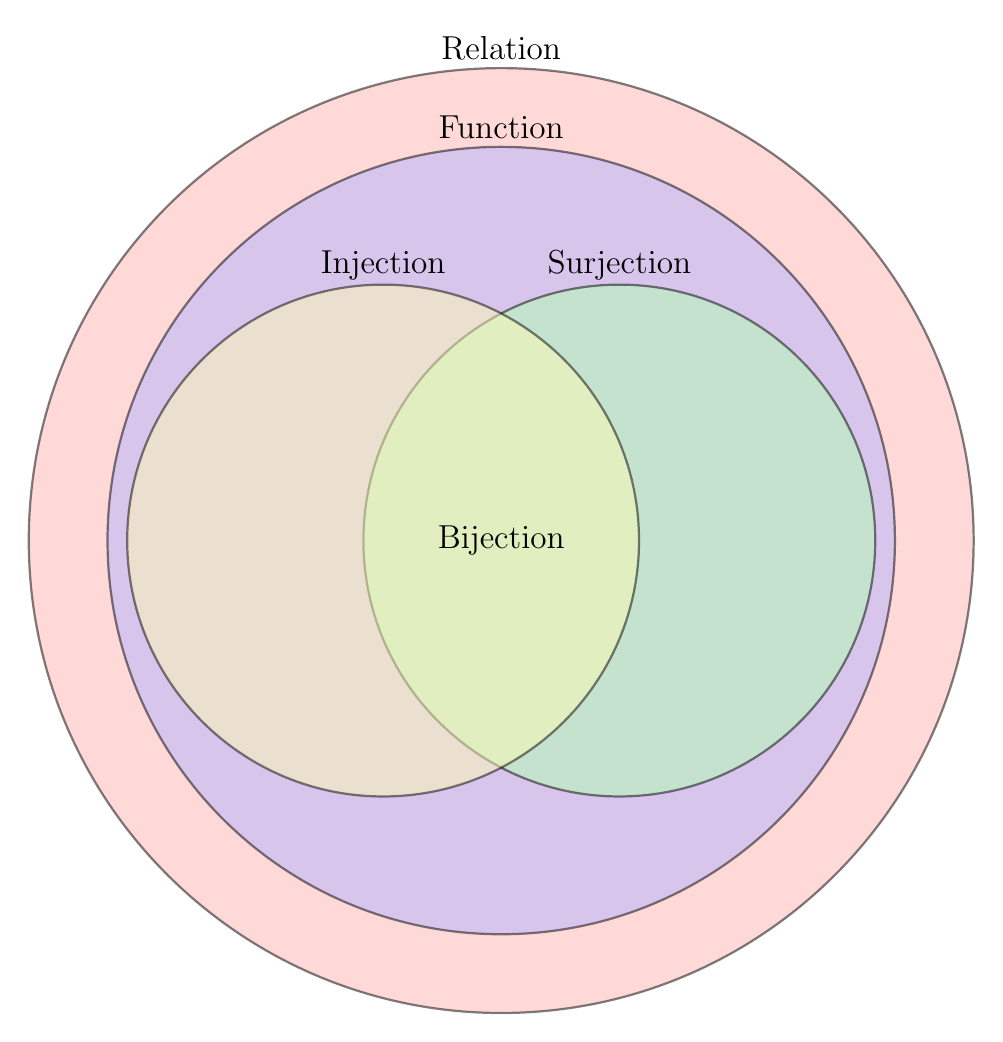
\begin{tikzpicture}
% Define circles
\draw[thick, fill=red!30, opacity=0.5] (0,0) circle (6cm); \node at (0, 6.25) {\large Relation};
\draw[thick, fill=blue!30, opacity=0.5] (0,0) circle (5cm); \node at (0, 5.25) {\large Function};
\draw[thick, fill=green!30, opacity=0.5] (1.5,0) circle (3.25cm); \node at (1.5, 3.5) {\large Surjection};
\draw[thick, fill=yellow!30, opacity=0.5] (-1.5,0) circle (3.25cm); \node at (-1.5, 3.5) {\large Injection};
%\draw[thick, fill=violet!30, opacity=0.5] (0,0) circle (1cm); 
\node at (0, 0) {\large Bijection};
\end{tikzpicture}}
\end{center}
\end{observation}

\section{Functions}
\defbox[Function]{
\begin{definition}
	Let $S$ and $T$ be sets. A \textbf{function} $f$ \textbf{from $\boldmath{S}$ to $\boldmath{T}$} is a relation on $S\times T$ satisfying as follows: \begin{enumerate}[(i)]
		\item (\textbf{Left-Total}\footnote{Every element of $S$ relates to some element of $T$.}) $\dom f=S$, \ie, \[
		s\in S\implies \exists t\in T:f(s)=t.
		\]
		\item (\textbf{Many-to-one}\footnote{Every element of $\dom{f}$ relates to no more than one element of its $\cdm{f}$.}) Let $s\in\dom{f}$ and $t_1,t_2\in\cdm{f}$. Then \[
		f(s)=t_1\land f(s)=t_2\implies s_1=s_2.
		\]
	\end{enumerate}
\end{definition}
}

\defbox[Domain, Codomain, and Range]{
\begin{definition}
\ \begin{itemize}
	\item \textbf{Domain:} The domain of a function \( f: A \to B \) is the set \( A \) of all possible input values for which the function is defined. Formally:
	\[
	\text{Domain}(f) = A
	\]
	\item \textbf{Co-domain:} The co-domain of a function \( f: A \to B \) is the set \( B \) which includes all potential output values. It is the target set for the function. Formally:
	\[
	\text{Co-domain}(f) = B
	\]
	\item \textbf{Range:} The range (or image) of a function \( f \) is the set of all actual output values produced by the function. It is a subset of the co-domain \( B \). Formally:
	\[
	\text{Range}(f) = f[A] = \{ f(a) \mid a \in A \} \subseteq B
	\]
\end{itemize}
\end{definition}
}
\begin{remark}
\ \\ \adjustbox{scale=.9, center}{
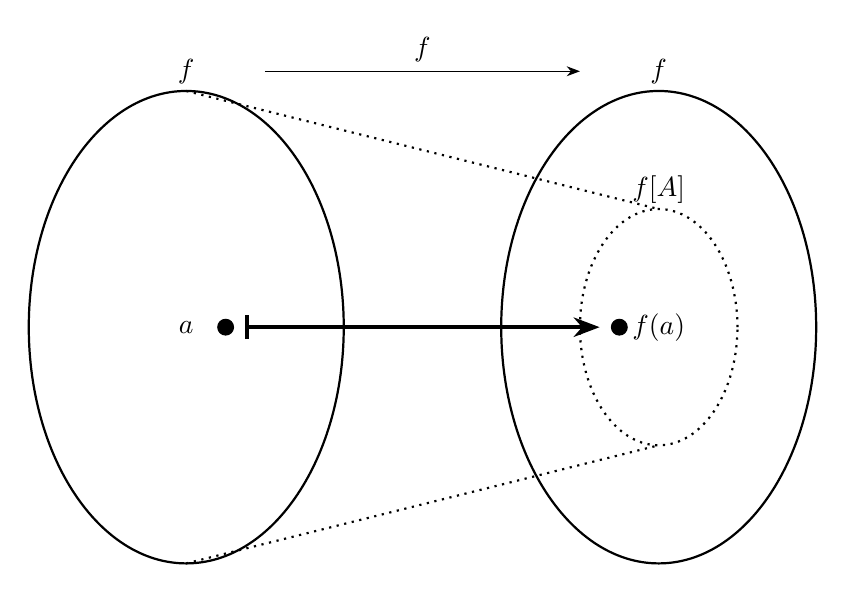
\begin{tikzpicture}
	% Draw the sets A and B
	\draw[thick] (-3,0) ellipse (2 and 3);
	\draw[thick] (3,0) ellipse (2 and 3);
	
	% Labels for sets
	\node at (-3, 3.25) {$\dom f$};
	\node at (3, 3.25) {$\cdm f$};
	
	% Draw the arrows representing the function
	\draw[-Stealth] (-2, 3.25) -- (2,3.25) node[midway, above] {$f$};
	\draw[thick, dotted] (-3,3) -- (3,1.5);
	\draw[thick, dotted] (-3,-3) -- (3,-1.5);
	
	\draw[fill] (-2.5,0) circle (.1);
	\draw[fill] (2.5,0) circle (.1);
	\draw[|-Stealth, line width=.5mm] (-2.25, 0) -- (2.25, 0);
	
	% Labels for elements in Domain
	\node at (-3, 0) {$a$};
	
	% Labels for elements in Co-domain
	\node at (3, 0) {$f(a)$};
	
	% Highlight the range
	\draw[thick, dotted] (3, 0) ellipse (1 and 1.5);
	
	% Label for the range
	\node at (3, 1.75) {$f[A]$};
\end{tikzpicture}}
\end{remark}

\section{Composition}
\defbox[Composition of Functions]{
\begin{definition}
Given two functions \( f \) and \( g \), where \( f: A \to B \) and \( g: B \to C \), the \textbf{composition} of \( g \) and \( f \), denoted by \( g \circ f \), is a function from \( A \) to \( C \) defined as follows:
\[
(g \circ f)(x) = g(f(x))
\]
for all \( x \in A \). That is, \[
\fullfunction{g\circ f}{A}{C}{a}{(g\circ f)(a)}
\]
\end{definition}}
\begin{remark}
\ \begin{itemize}
	\item \textbf{Functions}:
	\begin{itemize}
		\item Let \( f: B \to C \) be a function from set \( B \) to set \( C \).
		\item Let \( g: A \to B \) be a function from set \( A \) to set \( B \).
	\end{itemize}
	
	\item \textbf{Composition Definition}:
	\begin{itemize}
		\item The composition \( f \circ g \) is a function from \( A \) to \( C \).
		\item For each \( x \in A \), \( (f \circ g)(x) \) is defined as \( f(g(x)) \).
	\end{itemize}
	
	\item \textbf{Domain and Range}:
	\begin{itemize}
		\item The domain of the composite function \( f \circ g \) is \( A \).
		\item The range of the composite function \( f \circ g \) is a subset of \( C \).
	\end{itemize}
\end{itemize}
\end{remark}
\vspace{12pt}
\begin{remark}
Let \( G \) be a set of bijective functions from a set \( X \) to itself. Define the binary operation \(\circ\) to be the composition of functions. Then \( G \) under this operation is a group.
\begin{enumerate}
	\item \textbf{Closure}: If \( f, g \in G \), then \( f \circ g \in G \) because the composition of two bijective functions is bijective.
	
	\item \textbf{Associativity}: Function composition is associative. For any \( f, g, h \in G \),
	\[
	(f \circ g) \circ h = f \circ (g \circ h)
	\]
	\adjustbox{scale=.9, center}{
		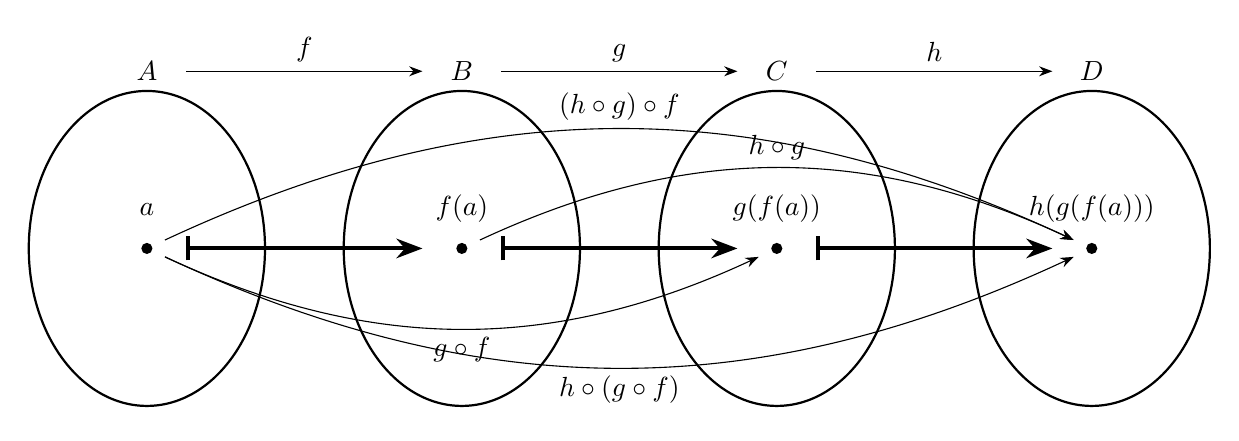
\begin{tikzpicture}
			% Draw the sets A and B
			\draw[thick] (-6,0) ellipse (1.5 and 2);
			\draw[thick] (-2,0) ellipse (1.5 and 2);
			\draw[thick] (2,0) ellipse (1.5 and 2);
			\draw[thick] (6,0) ellipse (1.5 and 2);
			
			% Labels for sets
			\node at (-6, 2.25) {$A$};
			\node at (-2, 2.25) {$B$};
			\node at (2, 2.25) {$C$};
			\node at (6, 2.25) {$D$};
			
			% Draw the arrows representing the function
			\draw[-Stealth] (-5.5, 2.25) -- (-2.5, 2.25) node[midway, above] {$f$};
			\draw[-Stealth] (-1.5, 2.25) -- (1.5, 2.25) node[midway, above] {$g$};
			\draw[-Stealth] (2.5, 2.25) -- (5.5, 2.25) node[midway, above] {$h$};
			\draw[|-Stealth, line width=.5mm] (-5.5, 0) -- (-2.5, 0);
			\draw[|-Stealth, line width=.5mm] (-1.5, 0) -- (1.5, 0);
			\draw[|-Stealth, line width=.5mm] (2.5, 0) -- (5.5, 0);
			
			% Labels for elements in Domain
			\node[fill, circle, inner sep=0.05cm] at (-6,0) (A) {};
			\node[fill, circle, inner sep=0.05cm] at (-2,0) (B) {};
			\node[fill, circle, inner sep=0.05cm] at (2,0) (C) {};
			\node[fill, circle, inner sep=0.05cm] at (6,0) (D) {};
			\node (A2) at (-6, 0.5) {$a$};
			\node (B2) at (-2, 0.5) {$f(a)$};
			\node (C2) at (2, 0.5) {$g(f(a))$};
			\node (D2) at (6, 0.5) {$h(g(f(a)))$};
			
			\draw[-Stealth, bend right=25pt, shorten <= 5pt, shorten >= 5pt] (A) to node[midway,below] {$g\circ f$} (C);
			\draw[-Stealth, bend right=25pt, shorten <= 5pt, shorten >= 5pt] (A) to node[midway,below] {$h\circ(g\circ f)$} (D);
			
			\draw[-Stealth, bend left=25pt, shorten <= 5pt, shorten >= 5pt] (A) to node[midway,above] {$(h\circ g)\circ f$} (D);
			\draw[-Stealth, bend left=25pt, shorten <= 5pt, shorten >= 5pt] (B) to node[midway,above] {$h\circ g$} (D);
	\end{tikzpicture}}
	\item \textbf{Identity Element}: The identity function \( \text{id}_A: A \to A \), defined by \( \text{id}_A(a) = a \) for all \( a \in A \), is the identity element in \( G \). For any \( f \in G \),
	\[
	f \circ \text{id}_A = f = \text{id}_A \circ f
	\]
	\begin{itemize}
		\item[] $f\circ \id_A:$
		\item[] $\id_A\circ f:$
		\item[] $f:$
	\end{itemize}
	\item \textbf{Inverse Element}: For each \( f \in G \), its inverse \( f^{-1} \) exists and is also a bijection from \( A \) to \( A \). It satisfies
	\[
	f \circ f^{-1} = \text{id}_A = f^{-1} \circ f
	\]
\end{enumerate}
\end{remark}

\section{Symmetric Group}
\begin{exercise}[Symmetric Group $S_2$]
The \textbf{symmetric group} \( S_2 \) is the group of all permutations of a two-element set. For a set \( X = \{1, 2\} \), the symmetric group \( S_2 \) consists of all bijective functions (permutations) from \( X \) to itself.

There are exactly two permutations of the set \( S = \{1, 2\} \):
\begin{itemize}
	\item \textbf{Identity Permutation} \( \text{id} \):
	\[
	\text{id}(1) = 1, \quad \text{id}(2) = 2
	\]
	This permutation leaves every element in its original position.\\
	\ \\
	\adjustbox{scale=.9, center}{
		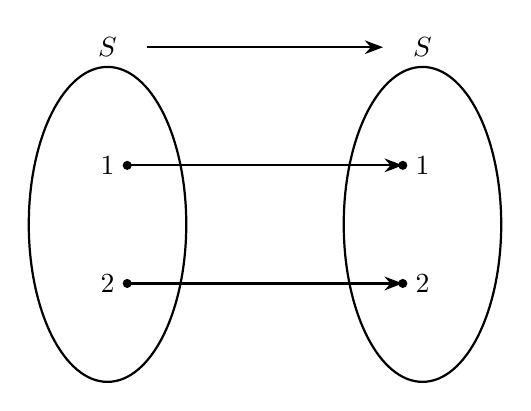
\begin{tikzpicture}
			% Draw the sets A and B
			\draw[thick] (-2,0) ellipse (1 and 2);
			\draw[thick] (2,0) ellipse (1 and 2);
			
			% Labels for sets
			\node at (-2, 2.25) {$S$};
			\node at (2, 2.25) {$S$};
			
%			% Draw the arrows representing the function
			\draw[-Stealth, thick] (-1.5, 2.25) -- (1.5,2.25) node[midway, above] {$\id$};
			
			\node (A) at (-2, .75) {$1$};
			\node (B) at (-2, -.75) {$2$};
			\draw[fill] (-1.75,.75) circle (.05);
			\draw[fill] (-1.75,-.75) circle (.05);
			
			\node (C) at (2, .75) {$1$};
			\node (D) at (2, -.75) {$2$};
			\draw[fill] (1.75,.75) circle (.05);
			\draw[fill] (1.75,-.75) circle (.05);
			
			\draw[-Stealth, thick] (-1.75, .75) -- (1.75, .75);
			\draw[-Stealth, thick] (-1.75, -.75) -- (1.75, -.75);
	\end{tikzpicture}}
	\item \textbf{Transposition} \( \sigma \):
	\[
	\sigma(1) = 2, \quad \sigma(2) = 1
	\]
	This permutation swaps the two elements.\\
	\ \\
	\adjustbox{scale=.9, center}{
		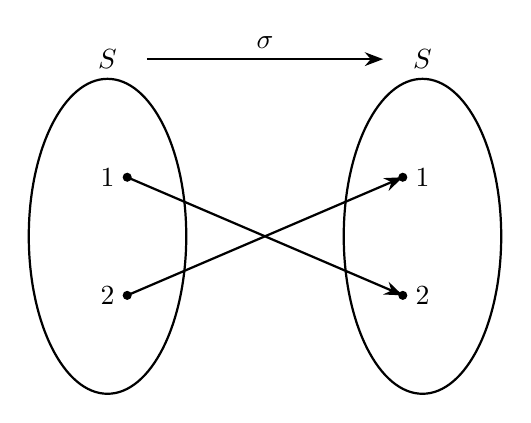
\begin{tikzpicture}
			% Draw the sets A and B
			\draw[thick] (-2,0) ellipse (1 and 2);
			\draw[thick] (2,0) ellipse (1 and 2);
			
			% Labels for sets
			\node at (-2, 2.25) {$S$};
			\node at (2, 2.25) {$S$};
			
			% Draw the arrows representing the function
			\draw[-Stealth, thick] (-1.5, 2.25) -- (1.5,2.25) node[midway, above] {$\sigma$};
			
			\node (A) at (-2, .75) {$1$};
			\node (B) at (-2, -.75) {$2$};
			\draw[fill] (-1.75,.75) circle (.05);
			\draw[fill] (-1.75,-.75) circle (.05);
			
			\node (C) at (2, .75) {$1$};
			\node (D) at (2, -.75) {$2$};
			\draw[fill] (1.75,.75) circle (.05);
			\draw[fill] (1.75,-.75) circle (.05);
			
			\draw[-Stealth, thick] (-1.75, .75) -- (1.75, -.75);
			\draw[-Stealth, thick] (-1.75, -.75) -- (1.75, .75);
	\end{tikzpicture}}
\end{itemize}

Therefore, the elements of \( S_2 \) can be written as:
\[
S_2 = \{ \text{id}, \sigma \}
\]

\end{exercise}
\vspace{12pt}
\begin{exercise}[Symmetric Group $S_3$]
	content...
\end{exercise}

\subsection*{Group Operation}

The group operation in \( S_2 \) is the composition of permutations. Given two permutations \( f \) and \( g \), their composition \( f \circ g \) is defined as:
\[
(f \circ g)(x) = f(g(x))
\]
for all \( x \in X \).

\subsection*{Group Table (Cayley Table)}

The Cayley table for \( S_2 \) describes the result of composing any two permutations:
\[
\begin{array}{c|cc}
	\circ & \text{id} & \sigma \\
	\hline
	\text{id} & \text{id} & \sigma \\
	\sigma & \sigma & \text{id} \\
\end{array}
\]

\subsection*{Group Axioms Verification}

\begin{itemize}
	\item \textbf{Closure}:
	\begin{itemize}
		\item The composition of any two elements in \( S_2 \) is also an element of \( S_2 \).
	\end{itemize}
	
	\item \textbf{Associativity}:
	\begin{itemize}
		\item Function composition is associative. For all \( f, g, h \in S_2 \),
		\[
		(f \circ g) \circ h = f \circ (g \circ h)
		\]
	\end{itemize}
	
	\item \textbf{Identity Element}:
	\begin{itemize}
		\item The identity permutation \(\text{id}\) acts as the identity element. For all \( f \in S_2 \),
		\[
		f \circ \text{id} = \text{id} \circ f = f
		\]
	\end{itemize}
	
	\item \textbf{Inverse Element}:
	\begin{itemize}
		\item Each element in \( S_2 \) has an inverse in \( S_2 \). Specifically,
		\[
		\text{id}^{-1} = \text{id}, \quad \sigma^{-1} = \sigma
		\]
	\end{itemize}
\end{itemize}
%	
%	\newpage
%	\chapter{Group Homomorphism}
%	% Group Homomorphism
\section{Exponentiation Function}

Consider the following groups:
\begin{itemize}
	\item The \textbf{additive group on integers} \((\mathbb{Z}, +)\):
	\begin{itemize}
		\item Set: \(\mathbb{Z}\)
		\item Operation: Addition (+)
		\item Identity Element: 0
		\item Inverses: For each \(a \in \mathbb{Z}\), the inverse is \(-a\).
	\end{itemize}
	
	\item The \textbf{multiplicative group on nonzero rational numbers} \((\mathbb{Q}^*, \cdot)\):
	\begin{itemize}
		\item Set: \(\mathbb{Q}^*\)
		\item Operation: Multiplication (\(\cdot\))
		\item Identity Element: 1
		\item Inverses: For each \(q \in \mathbb{Q}^*\), the inverse is \(q^{-1} = \frac{1}{q}\).
	\end{itemize}
\end{itemize}

We define the exponential function \( \exp : \mathbb{Z} \to \mathbb{Q}^* \) by:
\[
\exp(n) = 2^n \quad \text{for all} \ n \in \mathbb{Z}.
\]

\subsection*{Verification}

\paragraph{Homomorphism Property:}
\[
\exp(a + b) = 2^{a + b} = 2^a \cdot 2^b = \exp(a) \cdot \exp(b).
\]

\paragraph{Identity Element:}
\begin{itemize}
	\item In \((\mathbb{Z}, +)\), the identity element is 0.
	\item In \((\mathbb{Q}^*, \cdot)\), the identity element is 1.
\end{itemize}
\[
\exp(0) = 2^0 = 1.
\]

\paragraph{Inverses:}
\begin{itemize}
	\item For each \( n \in \mathbb{Z} \), the inverse of \( n \) in \(\mathbb{Z}\) is \(-n\).
	\item The inverse of \( \exp(n) = 2^n \) in \(\mathbb{Q}^*\) should be \( \exp(-n) = 2^{-n} \).
\end{itemize}
\[
\exp(-n) = 2^{-n} = \frac{1}{2^n} = (\exp(n))^{-1}.
\]

Thus, the exponential function \( \exp(n) = 2^n \) preserves the group structure between the additive group on integers \((\mathbb{Z}, +)\) and the multiplicative group on nonzero rational numbers \((\mathbb{Q}^*, \cdot)\).

\end{document}
%	
%	\newpage
%	\chapter{Linear Algebra and Group}
%	% Linear Algebra and Group
\begin{note}[General Definition of Vector Space]
The operations $+$ and $\cdot$ must satisfy the following properties for all $\mathbf{u}, \mathbf{v} \in V$ and $\alpha, \beta \in \mathbb{F}$:
\begin{enumerate}
	\item \textbf{Associativity of Addition}:
	\begin{equation*}
		(\mathbf{u} + \mathbf{v}) + \mathbf{w} = \mathbf{u} + (\mathbf{v} + \mathbf{w})
	\end{equation*}
	\item \textbf{Commutativity of Addition}:
	\begin{equation*}
		\mathbf{u} + \mathbf{v} = \mathbf{v} + \mathbf{u}
	\end{equation*}
	\item \textbf{Existence of Additive Identity}:
	\begin{equation*}
		\vec{u}\in V\implies\exists \mathbf{0} \in V:\mathbf{u} + \mathbf{0} = \mathbf{u}
	\end{equation*}
	\item \textbf{Existence of Additive Inverse}:
	\begin{equation*}
		\vec{u}\in V\implies \exists -\mathbf{u} \in V : \mathbf{u} + (-\mathbf{u}) = \mathbf{0}
	\end{equation*}
	\item \textbf{Distributivity of Scalar Multiplication over Vector Addition}:
	\begin{equation*}
		\alpha \cdot (\mathbf{u} + \mathbf{v}) = (\alpha \cdot \mathbf{u}) + (\alpha \cdot \mathbf{v})
	\end{equation*}
	\item \textbf{Distributivity of Scalar Multiplication over Field Addition}:
	\begin{equation*}
		(\alpha + \beta) \cdot \mathbf{u} = (\alpha \cdot \mathbf{u}) + (\beta \cdot \mathbf{u})
	\end{equation*}
	\item \textbf{Compatibility of Scalar Multiplication with Field Multiplication}:
	\begin{equation*}
		(\alpha \beta) \cdot \mathbf{u} = \alpha \cdot (\beta \cdot \mathbf{u})
	\end{equation*}
	\item \textbf{Identity Element of Scalar Multiplication}:
	\begin{equation*}
		1 \cdot \mathbf{u} = \mathbf{u}
	\end{equation*}
\end{enumerate}
\end{note}

\defbox[Linear Operation]{\begin{definition}
Let $V$ be a set over a field $\mathbb{F}$. We define the following linear operations on $V$:
\begin{enumerate}
	\item An \textbf{addition operation} 
	\begin{align*}
		+ : V \times V &\rightarrow V \\
		(\mathbf{u}, \mathbf{v}) &\mapsto \mathbf{u} + \mathbf{v}
	\end{align*}
	on $V$ such that $(V, +)$ is an abelian group.
		
	\item A \textbf{scalar multiplication operation} 
	\begin{align*}
		\cdot : \mathbb{F} \times V &\rightarrow V \\
		(\alpha, \mathbf{u}) &\mapsto \alpha \cdot \mathbf{u}
	\end{align*}
	on $V$. Here $0\cdot\vec{u}:=\vec{0}$ and $1\cdot\vec{u}:=\vec{u}$, \ie, \begin{align*}
		\cdot : \F \times V &\rightarrow V & \cdot : \F \times V &\rightarrow V \\
		(0, \mathbf{u}) &\mapsto \mathbf{0} & (1, \mathbf{u}) &\mapsto \mathbf{u}
	\end{align*}
\end{enumerate}
\end{definition}}
\begin{remark}
Consider \[
\cdot:\F\to[V\to V].
\] Then 
\begin{center}\adjustbox{scale=.9}{
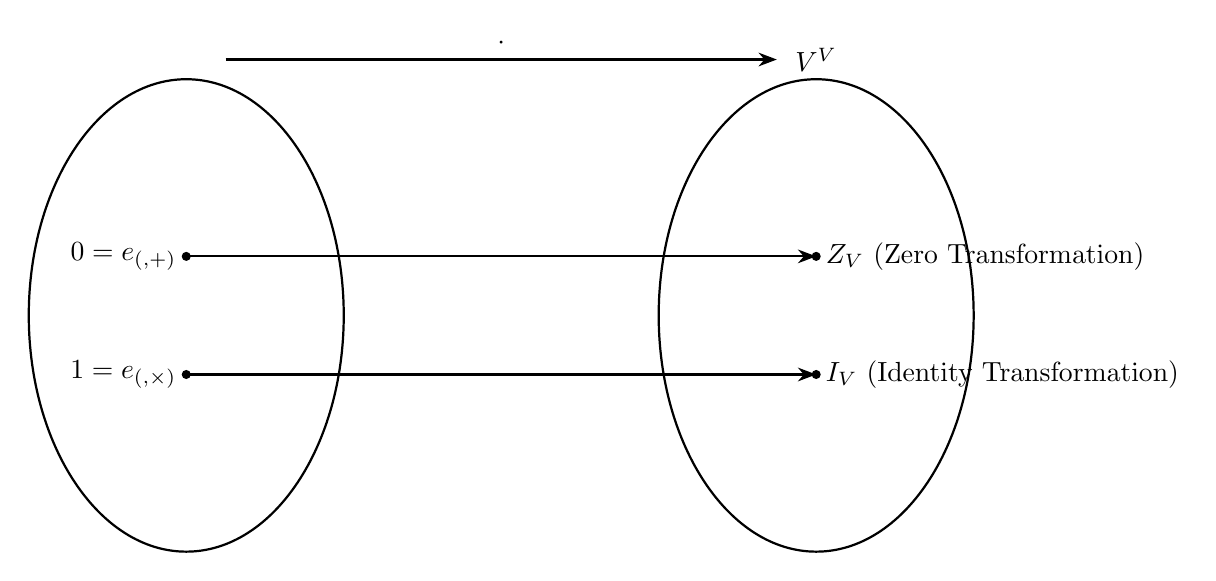
\begin{tikzpicture}
	% Draw the sets A and B
	\draw[thick] (-4,0) ellipse (2 and 3);
	\draw[thick] ( 4,0) ellipse (2 and 3);
	
	% Labels for sets
	\node at (-4, 3.25) {$\F$};
	\node at ( 4, 3.25) {$V^V$};
	
	% Draw the arrows representing the function
	\draw[-Stealth, thick] (-3.5, 3.25) -- (3.5,3.25) node[midway, above] {$\cdot$};
	\draw[fill] (-4,.75) circle (.05) node[left] {$0=e_{(\F,+)}$};
	\draw[fill] (-4,-.75) circle (.05) node[left] {$1=e_{(\F,\times)}$};
	
	\draw[fill] (4,.75) circle (.05) node[right] {$Z_V$ (Zero Transformation)};
	\draw[fill] (4,-.75) circle (.05) node[right] {$I_V$ (Identity Transformation)};
	
	\draw[-Stealth, thick] (-4, .75) -- (4, .75);
	\draw[-Stealth, thick] (-4, -.75) -- (4, -.75);
\end{tikzpicture}}
\end{center}
\end{remark}
\begin{remark}
	Let $V$ be a set over a field $\F$. Assume that, for $\vec{x},\vec{y}\in V$ and $\alpha,\beta\in F$, \[
	\alpha\cdot\vec{x} + \beta\cdot\vec{y}\in V.
	\] Then \[\begin{array}{rcll}
		\alpha=1=\beta &\implies &\vec{x} + \vec{y} \in V &\cdots\cdots\text{(Additivity)} \\
		\beta=0 &\implies &\alpha\cdot \vec{x} \in V &\cdots\cdots\text{(Homogeneity)}
	\end{array}
	\]
\end{remark}

\defbox[Vector Space]{\begin{definition}
A \textbf{vector space} \((V,+,\cdot)\), simply \( V \), over a field \( F \) is a set \( V \) together with two operations:
\begin{enumerate}
	\item \textbf{Vector Addition:} \[
	\fullfunction{+}{V\times V}{V}{(\vec{u},\vec{v})}{\vec{u}+\vec{v}},
	\] such that \( (V, +) \) forms an \underline{abelian group}.
	\item \textbf{Scalar Multiplication:} \[
	\fullfunction{\cdot}{F\times V}{V}{(a,\vec{u})}{a\cdot\vec{u}},
	\] such that \( (V, \cdot) \) satisfies the following properties:
	\begin{enumerate}
		\item \textbf{Distributivity of Scalar Multiplication with Respect to Vector Addition:} \[
		a \cdot (\mathbf{u} + \mathbf{v}) = (a \cdot \mathbf{u}) + (a \cdot \mathbf{v}).
		\]
		\item \textbf{Distributivity of Scalar Multiplication with Respect to Field Addition:} \[
		(a + b) \cdot \mathbf{v} = (a \cdot \mathbf{v}) + (b \cdot \mathbf{v}).
		\]
		\item \textbf{Associativity of Scalar Multiplication:} \[
		a \cdot (b \cdot \mathbf{v}) = (a \cdot b) \cdot \mathbf{v}.
		\]
		\item \textbf{Multiplicative Identity:} \[
		\vec{v}\in V\implies 1 \cdot \mathbf{v} = \mathbf{v},
		\] where 1 is the multiplicative identity in \( F \).
	\end{enumerate}
\end{enumerate}
\end{definition}}

\defbox[Linear Transformation]{\begin{definition}
Let \( V \) and \( W \) be vector spaces over the same field \( F \). A function \( T : V \to W \) is called a \textbf{linear transformation} (or linear map) if for all \( \mathbf{u}, \mathbf{v} \in V \) and all scalars \( a \in F \), the following two conditions are satisfied:

\begin{enumerate}
	\item \textbf{Additivity:} \[
	T(\mathbf{u} + \mathbf{v}) = T(\mathbf{u}) + T(\mathbf{v}).
	\]
	\item \textbf{Homogeneity of Scalar Multiplication:} \[
	T(a \cdot \mathbf{u}) = a \cdot T(\mathbf{u}).
	\]
\end{enumerate}
That is, \( T \) preserves the operations of vector addition and scalar multiplication.
\end{definition}}
\begin{remark}
	\[\begin{cases}
		\vec{u},\vec{v}\in V\\
		a,b\in F
	\end{cases}\implies
	\fullfunction{T}{V}{W}{a\cdot\vec{u}+b\cdot\vec{v}}{T(a\cdot\vec{u}+b\cdot\vec{v})=a\cdot T(\vec{u})+b\cdot T(\vec{v})}
	\]
\end{remark}
\begin{remark}
Given that \( T : V \to W \) is a linear transformation, the following properties hold:
\begin{enumerate}
	\item \( T(\mathbf{0}_V) = \mathbf{0}_W \), where \( \mathbf{0}_V \) and \( \mathbf{0}_W \) are the zero vectors in \( V \) and \( W \), respectively.
	\item \( T\left(\sum_{i=1}^n a_i \mathbf{u}_i\right) = \sum_{i=1}^n a_i T(\mathbf{u}_i) \) for any finite set of vectors \( \mathbf{u}_1, \mathbf{u}_2, \ldots, \mathbf{u}_n \in V \) and scalars \( a_1, a_2, \ldots, a_n \in F \).
\end{enumerate}
\end{remark}
\begin{remark}
\ \begin{center}
\begin{tikzpicture}[auto, node distance=2cm, thick, >=Stealth]
	% Vector Addition
	\node (O1) at (0,0) {};
	\node (U) at (2,1) {};
	\node (V) at (1,2) {};
	\node (U+V) at ($(U) + (V)$) {};
	
	\node (TO1) at (0,-5) {};
	\node (TU) at (2,-4) {};
	\node (TV) at (1,-3) {};
	\node (TU+TV) at (3,-2) {};
	
	% Vectors for Addition
	\draw[->] (O1.center) -- (U.center) node[midway, below right] {$\mathbf{u}$};
	\draw[->] (O1.center) -- (V.center) node[midway, above left] {$\mathbf{v}$};
	\draw[->, dashed] (U.center) -- (U+V.center) node[midway, above right] {};
	\draw[->, dashed] (V.center) -- (U+V.center) node[midway, below left] {};
	\draw[->, very thick, magenta] (O1.center) -- (U+V.center) node[midway, above] {};
	
	\draw[->] (TO1.center) -- (TU.center) node[midway, below right] {$T(\mathbf{u})$};
	\draw[->] (TO1.center) -- (TV.center) node[midway, above left] {$T(\mathbf{v})$};
	\draw[->, dashed] (TU.center) -- (TU+TV.center) node[midway, above right] {};
	\draw[->, dashed] (TV.center) -- (TU+TV.center) node[midway, below left] {};
	\draw[->, very thick, magenta] (TO1.center) -- (TU+TV.center) node[midway, above] {};
	
	% Points for Addition
	\fill (O1) circle (2pt) node[below left] {$\mathbf{O}$};
	\fill (U) circle (2pt) node[below right] {};
	\fill (V) circle (2pt) node[above left] {};
	\fill (U+V) circle (2pt) node[above right] {\textcolor{magenta}{$\mathbf{u} + \mathbf{v}$}};
	
	\fill (TO1) circle (2pt) node[below left] {$\mathbf{O}$};
	\fill (TU) circle (2pt) node[below right] {};
	\fill (TV) circle (2pt) node[above left] {};
	\fill (TU+TV) circle (2pt) node[above right] {\textcolor{magenta}{$T(\mathbf{u}) + T(\mathbf{v})$}};
	
	% Scalar Multiplication
	\node (O2) at (7,0) {};
	\node (U2) at (9,1) {};
	\node (AU2) at ($(O2)!2!(U2)$) {};
	
	\node (TO2) at (7,-5) {};
	\node (TU2) at (9,-4) {};
	\node (TAU2) at (11,-3) {};
	
	% Vectors for Multiplication
	\draw[->] (O2.center) -- (U2.center) node[midway, below right] {$\mathbf{u}$};
	\draw[->, very thick, magenta] (O2.center) -- (AU2.center) node[midway, above] {};
	
	\draw[->] (TO2.center) -- (TU2.center) node[midway, below right] {$T(\mathbf{u})$};
	\draw[->, very thick, magenta] (TO2.center) -- (TAU2.center) node[midway, above] {};
	
	% Points for Multiplication
	\fill (O2) circle (2pt) node[below left] {$\mathbf{O}$};
	\fill (U2) circle (2pt) node[below right] {};
	\fill (AU2) circle (2pt) node[above] {\textcolor{magenta}{$a \cdot \mathbf{u}$}};
	
	\fill (TO2) circle (2pt) node[below left] {$\mathbf{O}$};
	\fill (TU2) circle (2pt) node[below right] {};
	\fill (TAU2) circle (2pt) node[above] {\textcolor{magenta}{$a \cdot T(\mathbf{u})$}};
	
	% Mapping
	\draw[draw=black] (-1, 3.5) rectangle (6,-.5);
	\draw[draw=black] (-1, -1.25) rectangle (6,-5.75);
	\draw[draw=black] (6.25, 3.5) rectangle (13,-.5);
	\draw[draw=black] (6.25, -1.25) rectangle (13,-5.75);
%	\draw[|-Stealth, thick, shorten <= 10pt, shorten >= 5pt] (3, 3) to node[midway, right] {$T(\vec{u}+\vec{v})$} (3,-2);
%	\draw[|-Stealth, thick, shorten <= 10pt, shorten >= 5pt] (11, 2) to node[midway, right] {$T(a\cdot\vec{u})$} (11,-3);
\end{tikzpicture}
%\vspace{36pt}
%\begin{tikzpicture}[auto, node distance=2cm, thick, >=Stealth]
%	% Vector Addition
%	\node (O1) at (0,0) {};
%	\node (U) at (2,1) {};
%	\node (V) at (1,2) {};
%	\node (U+V) at ($(U) + (V)$) {};
%	
%	% Vectors for Addition
%	\draw[->] (O1.center) -- (U.center) node[midway, below right] {$T(\mathbf{u})$};
%	\draw[->] (O1.center) -- (V.center) node[midway, above left] {$T(\mathbf{v})$};
%	\draw[->, dashed] (U.center) -- (U+V.center) node[midway, above right] {};
%	\draw[->, dashed] (V.center) -- (U+V.center) node[midway, below left] {};
%	\draw[->, very thick, magenta] (O1.center) -- (U+V.center) node[midway, above] {};
%	
%	% Points for Addition
%	\fill (O1) circle (2pt) node[below left] {$\mathbf{O}$};
%	\fill (U) circle (2pt) node[below right] {};
%	\fill (V) circle (2pt) node[above left] {};
%	\fill (U+V) circle (2pt) node[above right] {\textcolor{magenta}{$T(\mathbf{u}) + T(\mathbf{v})$}};
%	
%	% Scalar Multiplication
%	\node (O2) at (7,0) {};
%	\node (U2) at (9,1) {};
%	\node (AU2) at ($(O2)!2!(U2)$) {};
%	
%	% Vectors for Multiplication
%	\draw[->] (O2.center) -- (U2.center) node[midway, below right] {$T(\mathbf{u})$};
%	\draw[->, very thick, magenta] (O2.center) -- (AU2.center) node[midway, above] {};
%	
%	% Points for Multiplication
%	\fill (O2) circle (2pt) node[below left] {$\mathbf{O}$};
%	\fill (U2) circle (2pt) node[below right] {};
%	\fill (AU2) circle (2pt) node[above] {\textcolor{magenta}{$a \cdot T(\mathbf{u})$}};
%\end{tikzpicture}
\end{center}
\end{remark}
\begin{remark}[\bf Dimension]
\ \begin{itemize}
	\item (\textbf{Finite-Dimensional Vector Spaces}) A finite-dimensional vector space \( V \) over a field \( F \) with dimension \( n \) is always isomorphic to \( F^n \).
	\item (\textbf{Basis and Isomorphism}) \begin{itemize}
		\item Let \( \{\mathbf{e}_1, \mathbf{e}_2, \ldots, \mathbf{e}_n\} \) be a basis for \( V \).
		\item Any vector \( \mathbf{v} \in V \) can be uniquely expressed as:
		\[
		\mathbf{v} = a_1 \mathbf{e}_1 + a_2 \mathbf{e}_2 + \cdots + a_n \mathbf{e}_n,
		\]
		where \( a_i \in F \) for \( i = 1, 2, \ldots, n \).
		\item The map:
		\[
		\varphi : V \to F^n, \quad \mathbf{v} \mapsto (a_1, a_2, \ldots, a_n)
		\]
		is a linear isomorphism.
	\end{itemize}
	\item (\textbf{Infinite-Dimensional Vector Spaces}) Infinite-dimensional vector spaces are more complex and are not isomorphic to \( F^n \) for any finite \( n \).
	\item (\textbf{Examples and Considerations}) \begin{itemize}
		\item \textbf{Function Spaces}: Spaces like the set of all polynomials \( \mathbb{P} \) or the space of continuous functions \( C([0, 1]) \).
		\item \textbf{Hilbert Spaces}: Spaces such as \( \ell^2 \) (space of square-summable sequences).
		\item \textbf{Isomorphisms}: Infinite-dimensional vector spaces may be isomorphic to structures like \( F^\infty \) (sequences with only finitely many non-zero entries) or \( F^{(\infty)} \) (the direct sum of infinitely many copies of \( F \)).
	\end{itemize}
\end{itemize}
\end{remark}


%	
%	From the standpoint of solving equations, the algebraic structures we have discussed are interconnected in the following ways:
%	
%	\subsection*{Group}
%	A \textbf{group} provides a foundation for solving equations involving a single operation. The group structure ensures that every element has an inverse, allowing us to "undo" operations and solve equations. For instance, in the group of integers \( (\mathbb{Z}, +) \), the equation \( x + a = b \) can be solved as \( x = b - a \).
%	
%	\subsection*{Ring}
%	A \textbf{ring} extends the concept of a group by introducing a second operation, typically multiplication, in addition to addition. Rings allow us to solve more complex equations that involve both addition and multiplication. For example, solving polynomial equations \( f(x) = 0 \) where \( f(x) \) is a polynomial with coefficients in a ring \( R \).
%	
%	\subsection*{Field}
%	A \textbf{field} is a ring with additional properties that make division possible (except by zero). This structure is crucial for solving linear equations and systems of linear equations. In a field \( F \), any linear equation \( ax = b \) (where \( a \neq 0 \)) can be solved as \( x = a^{-1}b \), where \( a^{-1} \) is the multiplicative inverse of \( a \).
%	
%	\subsection*{Vector Space}
%	A \textbf{vector space} over a field \( F \) is a set of vectors that can be added together and scaled by elements of \( F \). Vector spaces provide a framework for solving linear systems of equations. Solutions to systems of linear equations can be understood as finding vectors \( \mathbf{x} \in V \) such that \( A\mathbf{x} = \mathbf{b} \), where \( A \) is a matrix and \( \mathbf{b} \) is a vector in \( V \).
%	
%	\subsection*{Module}
%	A \textbf{module} is a generalization of vector spaces where the scalars come from a ring instead of a field. Modules allow us to solve equations in contexts where the coefficients are not from a field, such as systems of linear equations with integer coefficients. For example, solving \( A\mathbf{x} = \mathbf{b} \) where \( A \) is a matrix with entries from a ring \( R \) and \( \mathbf{x}, \mathbf{b} \in M \).
%	
%	\subsection*{Algebra}
%	An \textbf{algebra} over a field \( F \) combines the structures of a vector space and a ring. Algebras provide a framework for solving polynomial equations and other equations involving both addition and multiplication of vectors. In an algebra \( A \), we can solve equations like \( x^2 + ax + b = 0 \) using techniques from both linear algebra and ring theory.
%	
%	\subsection*{Summary}
%	The conceptual connection between these structures is rooted in the increasing complexity and capability they offer for solving equations:
%	\begin{itemize}
%		\item \textbf{Groups} provide a way to solve equations with a single operation.
%		\item \textbf{Rings} introduce a second operation, allowing for more complex equations.
%		\item \textbf{Fields} enable division, which is essential for solving linear equations.
%		\item \textbf{Vector spaces} over fields extend these concepts to systems of linear equations.
%		\item \textbf{Modules} generalize vector spaces to allow coefficients from rings.
%		\item \textbf{Algebras} integrate vector space and ring structures, enabling the solution of polynomial and other complex equations.
%	\end{itemize}
%	
%	\newpage
%	\chapter*{LaTex Practice}
%	\begin{itemize}
	\item \textbf{Block Size}: $n$ (number of bits in a block)
	\item \textbf{Key Size}: $k$ (number of bits in the key)
\end{itemize}
\begin{align*}
	E:\boxed{\set{0,1}^k\times\set{0,1}^n}\to\set{0,1}^n \\
	D:\boxed{\set{0,1}^k\times\set{0,1}^n}\to\set{0,1}^n
\end{align*}
\adjustbox{scale=.9, center}{
	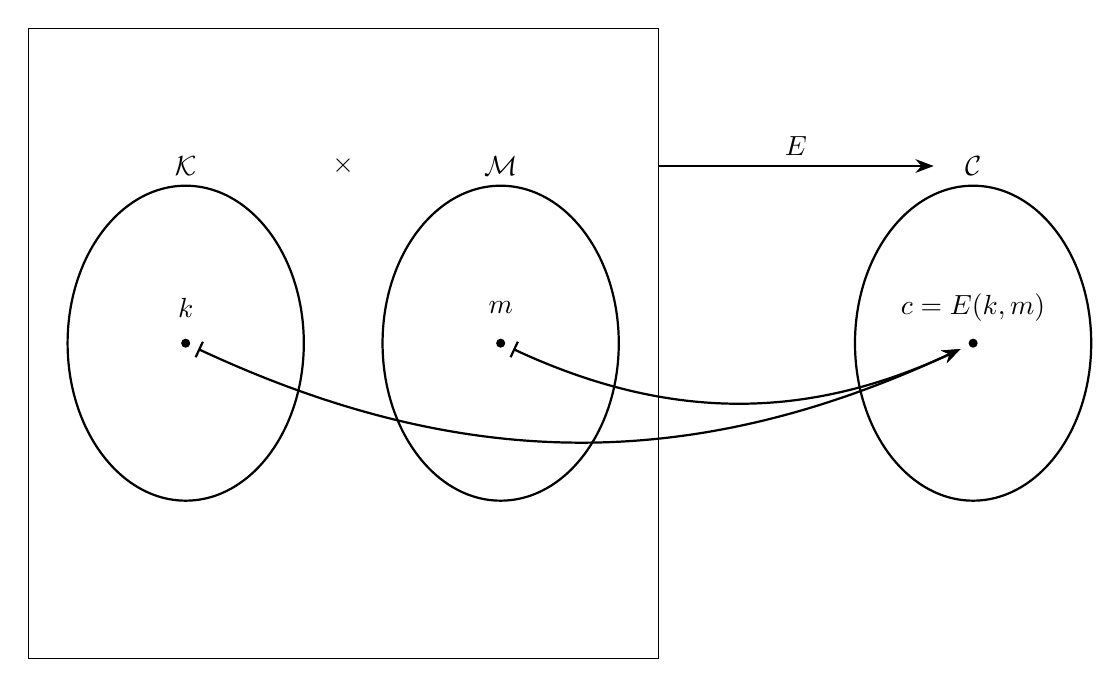
\begin{tikzpicture}
		% Draw the sets A and B
		\draw[thick] (-6,0) ellipse (1.5 and 2);
		\draw[thick] (-2,0) ellipse (1.5 and 2);
		\draw[thick] (4,0) ellipse (1.5 and 2);
		\draw[draw=black] (-8, 4) rectangle (0,-4);
		% Labels for sets
		\node at (-6, 2.25) {$\mathcal{K}$};
		\node at (-4, 2.25) {$\times$};
		\node at (-2, 2.25) {$\mathcal{M}$};
		\node at (4, 2.25) {$\mathcal{C}$};
		
		% Draw the arrows representing the function
		\draw[-Stealth, thick] (0, 2.25) -- (3.5,2.25) node[midway, above] {$E$};
		
		\node (K) at (-6, .45) {$k$};
		\node (M) at (-2, .45) {$m$};
		\node (C) at (4, .45) {$c=E(k,m)$};
		\draw[fill] (-6,0) circle (.05);
		\draw[fill] (-2,0) circle (.05);
		\draw[fill] (4,0) circle (.05);
		
		\draw[|-Stealth, thick, bend right=25pt, shorten <= 5pt, shorten >= 5pt] (-6, 0) to node[midway,below] {} (4,0);
		\draw[|-Stealth, thick, bend right=25pt, shorten <= 5pt, shorten >= 5pt] (-2, 0) to node[midway,below] {} (4,0);
\end{tikzpicture}}
\begin{align*}
	E:\set{0,1}^k\to\boxed{\set{0,1}^n\to\set{0,1}^n} \\
	D:\set{0,1}^k\to\boxed{\set{0,1}^n\to\set{0,1}^n}
\end{align*}
\adjustbox{scale=.9, center}{
	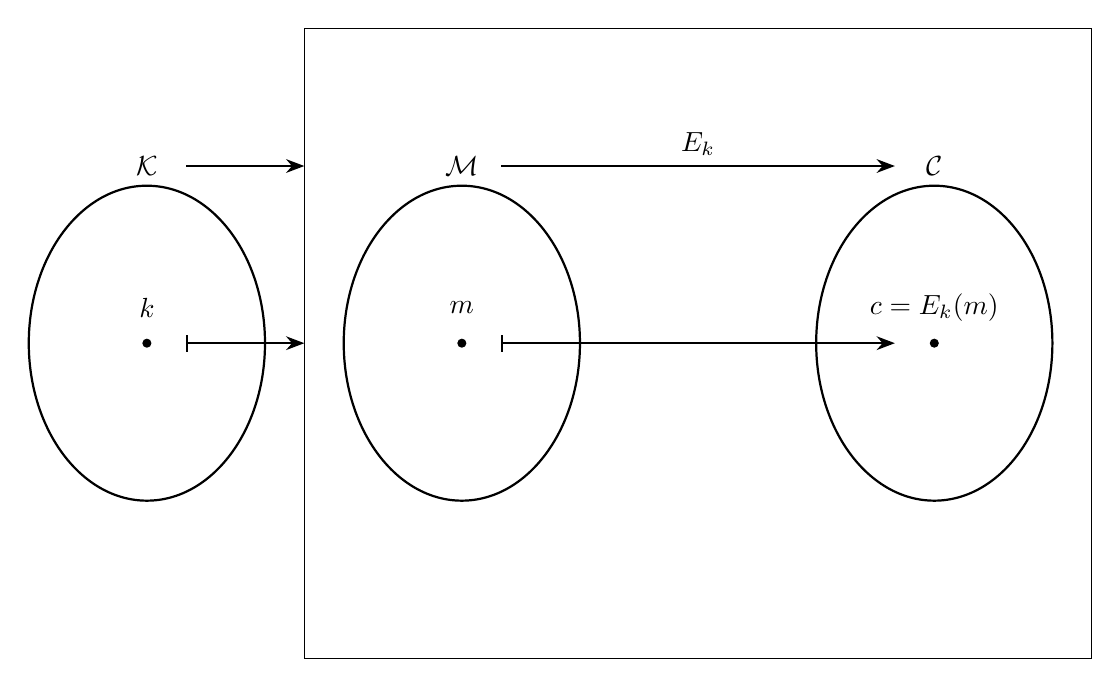
\begin{tikzpicture}
		% Draw the sets A and B
		\draw[thick] (-6,0) ellipse (1.5 and 2);
		\draw[thick] (-2,0) ellipse (1.5 and 2);
		\draw[thick] (4,0) ellipse (1.5 and 2);
		\draw[draw=black] (-4, 4) rectangle (6,-4);
		% Labels for sets
		\node at (-6, 2.25) {$\mathcal{K}$};
		\node at (-2, 2.25) {$\mathcal{M}$};
		\node at (4, 2.25) {$\mathcal{C}$};
		
		% Draw the arrows representing the function
		\draw[-Stealth, thick] (-1.5, 2.25) -- (3.5,2.25) node[midway, above] {$E_k$};
		\draw[-Stealth, thick] (-5.5, 2.25) -- (-4,2.25) node[midway, above] {};
		
		\node (K) at (-6, .45) {$k$};
		\node (M) at (-2, .45) {$m$};
		\node (C) at (4, .45) {$c=E_k(m)$};
		\draw[fill] (-6,0) circle (.05);
		\draw[fill] (-2,0) circle (.05);
		\draw[fill] (4,0) circle (.05);
		
		\draw[|-Stealth, thick] (-5.5, 0) to node[midway,below] {} (-4,0);
		\draw[|-Stealth, thick] (-1.5, 0) to node[midway,below] {} (3.5,0);
\end{tikzpicture}}
%	
%	% Appendix
%	\newpage
%	\appendix
%	\chapter{Preliminaries}
\section{Sets, Cartesian Products, and Relations}

\subsection{Sets and Ordered Pairs}

\subsection*{Set}

A \textbf{set} is a well-defined collection of distinct objects, called elements or members of the set. Sets are one of the most fundamental concepts in mathematics.

\defbox[Set]{
\begin{definition}
	A \textbf{set} is a well-defined collection of distinct objects, considered as an object in its own right. Sets are usually denoted by capital letters, and the elements are listed within curly braces.
\end{definition}
}
\begin{example}
For example:
\[
A = \{1, 2, 3\}
\]
This denotes a set \(A\) containing the elements 1, 2, and 3.
\end{example}
\vspace{12pt}
\begin{note}[Properties]
\ \begin{itemize}
	\item \textbf{No Repetition}: Each element in a set appears only once.
	\item \textbf{Order Irrelevance}: The order of elements in a set does not matter. For instance, \(\{1, 2, 3\} = \{3, 2, 1\}\).
	\item \textbf{Membership}: If an element \(a\) is in a set \(A\), we write \(a \in A\).
\end{itemize}
\end{note}
\vspace{12pt}
\begin{note}[Types of Sets]
\ \begin{itemize}
	\item \textbf{Finite and Infinite Sets}: A set with a finite number of elements is finite; otherwise, it is infinite.
	\item \textbf{Subset}: A set \(A\) is a subset of a set \(B\) if every element of \(A\) is also an element of \(B\), denoted \(A \subseteq B\).
	\item \textbf{Power Set}: The power set of \(A\) is the set of all subsets of \(A\), denoted \(\mathcal{P}(A)\).
\end{itemize}
\end{note}

\subsection*{Ordered Pair}

An \textbf{ordered pair} is a fundamental concept in mathematics used to combine two elements in a specific order. The notation for an ordered pair is \((a, b)\), where \(a\) is the first element and \(b\) is the second element.

\defbox[Ordered Pair]{
\begin{definition}
	An \textbf{ordered pair} \((a, b)\) is a collection of two elements where the order of the elements matters. This is in contrast to a set, where the order of elements does not matter.
\end{definition}
}
\begin{remark}
	\ \begin{itemize}
		\item The ordered pair \((a, b)\) is not the same as \((b, a)\) unless \(a = b\).
		\item Formally, the ordered pair \((a, b)\) can be defined using sets to ensure the distinction from unordered pairs. One common definition is:
		\[
		(a, b) = \{ \{a\}, \{a, b\} \}
		\]
		This definition ensures that:
		\[
		(a, b) = (c, d) \iff a = c \ \text{and} \ b = d
		\]
	\end{itemize}
\end{remark}
\vspace{12pt}
\begin{note}[Properties]
\begin{itemize}
	\item \textbf{Uniqueness}: Each ordered pair \((a, b)\) is unique if either \(a\) or \(b\) is unique.
	\item \textbf{Order}: The order of elements in an ordered pair is significant.
\end{itemize}
\end{note}

\subsection{Cartesian Product and Relation}

\subsection*{Cartesian Product}

The \textbf{Cartesian product} is a fundamental concept in set theory, used to define the set of all possible ordered pairs from two sets.

\defbox[Cartesian Product]{
Given two sets \( A \) and \( B \), the Cartesian product \( A \times B \) is defined as the set of all ordered pairs \((a, b)\) where \( a \in A \) and \( b \in B \). Formally,
\[
A \times B = \{ (a, b) \mid a \in A \ \text{and} \ b \in B \}
\]
}
\vspace{12pt}
\begin{note}[Properties]
\ \begin{itemize}
	\item \textbf{Order Matters}: The pair \((a, b)\) is different from the pair \((b, a)\) unless \(a = b\).
	\item \textbf{Empty Set}: If either \(A\) or \(B\) is the empty set \(\emptyset\), then \(A \times B\) is also empty:
	\[
	A \times \emptyset = \emptyset \quad \text{and} \quad \emptyset \times B = \emptyset
	\]
\end{itemize}
\end{note}
\begin{example}
\ \begin{enumerate}
	\item If \( A = \{1, 2\} \) and \( B = \{x, y\} \), then
	\[
	A \times B = \{ (1, x), (1, y), (2, x), (2, y) \}
	\]
	
	\item If \( A = \{a, b\} \) and \( B = \{1, 2, 3\} \), then
	\[
	A \times B = \{ (a, 1), (a, 2), (a, 3), (b, 1), (b, 2), (b, 3) \}
	\]
\end{enumerate}
\end{example}

\subsection*{Relation}

A \textbf{relation} generalizes the concept of Cartesian product to establish connections between elements of two sets.

\defbox[Relation]{
\begin{definition}
	A relation \( R \) from a set \( A \) to a set \( B \) is a subset of the Cartesian product \( A \times B \). Formally,
	\[
	R \subseteq A \times B
	\]
	This means that a relation \( R \) consists of ordered pairs \((a, b)\) where \(a \in A\) and \(b \in B\).
\end{definition}
}
\vspace{12pt}
\begin{note}[Properties of Relations]
\ \begin{itemize}
	\item \textbf{Domain and Range}:
	\begin{itemize}
		\item The \textbf{domain} of \( R \) is the set of all \( a \in A \) such that there exists \( b \in B \) with \((a, b) \in R\).
		\[
		\text{Domain}(R) = \{ a \in A \mid \exists b \in B, \ (a, b) \in R \}
		\]
		\item The \textbf{range} of \( R \) is the set of all \( b \in B \) such that there exists \( a \in A \) with \((a, b) \in R\).
		\[
		\text{Range}(R) = \{ b \in B \mid \exists a \in A, \ (a, b) \in R \}
		\]
	\end{itemize}
	
	\item \textbf{Inverse Relation}: The inverse of a relation \( R \), denoted \( R^{-1} \), is the set of all pairs \((b, a)\) such that \((a, b) \in R\):
	\[
	R^{-1} = \{ (b, a) \mid (a, b) \in R \}
	\]
	
	\item \textbf{Composition of Relations}: Given a relation \( R \) from \( A \) to \( B \) and a relation \( S \) from \( B \) to \( C \), the composition \( S \circ R \) is a relation from \( A \) to \( C \) defined by:
	\[
	S \circ R = \{ (a, c) \mid \exists b \in B, \ (a, b) \in R \ \text{and} \ (b, c) \in S \}
	\]
\end{itemize}
\end{note}

\vspace{12pt}
\begin{note}[Types of Relations]
\ \begin{itemize}
	\item \textbf{Binary Relation}: A relation involving two sets, as defined above.
	\item \textbf{Unary Relation}: A relation on a single set \( A \) is simply a subset of \( A \).
	\item \textbf{Ternary and Higher Relations}: Relations involving three or more sets, defined as subsets of the Cartesian product of those sets.
\end{itemize}
\end{note}

\begin{example}
	\ \begin{enumerate}
		\item If \( A = \{1, 2, 3\} \) and \( B = \{a, b\} \), a possible relation \( R \) from \( A \) to \( B \) could be:
		\[
		R = \{ (1, a), (2, b), (3, a) \}
		\]
		\begin{itemize}
			\item Domain: \(\{1, 2, 3\}\)
			\item Range: \(\{a, b\}\)
		\end{itemize}
		
		\item Consider the relation \( R \) on set \( A = \{1, 2, 3\} \) defined by:
		\[
		R = \{ (1, 2), (2, 3), (3, 1) \}
		\]
		\begin{itemize}
			\item Domain: \(\{1, 2, 3\}\)
			\item Range: \(\{1, 2, 3\}\)
			\item Inverse Relation: \( R^{-1} = \{ (2, 1), (3, 2), (1, 3) \} \)
		\end{itemize}
	\end{enumerate}
\end{example}

\section{Rational Number and Equivalence Class}

We define the equivalence relation \((a, b) \sim (c, d)\) on the set \(\mathbb{Z} \times \mathbb{Z}^*\) as:
\[
(a, b) \sim (c, d) \iff ad = bc
\]
\begin{proof}
To prove that \(\sim\) is an equivalence relation, we must show it is reflexive, symmetric, and transitive.
\begin{itemize}
	\item \textbf{Reflexive}: A relation \(\sim\) is reflexive if every element is related to itself.
	
	For any \((a, b) \in \mathbb{Z} \times \mathbb{Z}^*\), we need to show that \((a, b) \sim (a, b)\).
	\[
	(a, b) \sim (a, b) \iff ab = ba
	\]
	This is true because \(ab = ba\) holds for all integers \(a\) and \(b\).
	Thus, the relation is reflexive.
	\item \textbf{Symmetric}: A relation \(\sim\) is symmetric if whenever \((a, b) \sim (c, d)\), then \((c, d) \sim (a, b)\).
	
	Assume \((a, b) \sim (c, d)\). This means:
	\[
	ad = bc
	\]
	We need to show that \((c, d) \sim (a, b)\).
	\[
	(c, d) \sim (a, b) \iff cd = da
	\]
	Since \(ad = bc\), we have \(cd = da\) by the commutative property of multiplication.
	Thus, the relation is symmetric.
	\item \textbf{Transitive}: A relation \(\sim\) is transitive if whenever \((a, b) \sim (c, d)\) and \((c, d) \sim (e, f)\), then \((a, b) \sim (e, f)\).
	
	Assume \((a, b) \sim (c, d)\) and \((c, d) \sim (e, f)\). This means:
	\[
	ad = bc \quad \text{and} \quad cf = de
	\]
	We need to show that \((a, b) \sim (e, f)\).
	\[
	(a, b) \sim (e, f) \iff af = be
	\]
	From \(ad = bc\), we have \(d = \frac{bc}{a}\) (assuming \(a \neq 0\)). Substituting \(d\) into \(cf = de\):
	\[
	c f = \left(\frac{bc}{a}\right) e
	\]
	Multiplying both sides by \(a\):
	\[
	a c f = b c e
	\]
	Since \(c \neq 0\):
	\[
	a f = b e
	\]
	Thus, \((a, b) \sim (e, f)\), proving that the relation is transitive.	
\end{itemize}
\end{proof}

Since the relation \((a, b) \sim (c, d) \iff ad = bc\) is reflexive, symmetric, and transitive, it is an equivalence relation on \(\mathbb{Z} \times \mathbb{Z}^*\).


The equivalence relation \((a, b) \sim (c, d) \iff ad = bc\) naturally connects to the division of the set of pairs of integers into equivalence classes, where each equivalence class represents a unique rational number.

An equivalence class \([(a, b)]\) under this relation consists of all pairs \((c, d)\) such that \((a, b) \sim (c, d)\). This can be interpreted as:
\[
[(a, b)] = \{ (c, d) \mid ad = bc \}
\]

Each equivalence class \([(a, b)]\) corresponds to the rational number \(\frac{a}{b}\), and different pairs \((a, b)\) and \((c, d)\) represent the same rational number if and only if they belong to the same equivalence class.

\begin{example}
Consider \((1, 2)\), \((2, 4)\), \((3, 6)\), \((-1, -2)\), \((1, -2)\)
\begin{itemize}
	\item (Class of $(1,2)$)
\[
[1, 2] = \{ (c, d) \in \mathbb{Z} \times \mathbb{Z}^* \mid 1d = 2c \} = \{ (1, 2), (2, 4), (3, 6), (-1, -2), \ldots \}
\]
This class represents the rational number \(\frac{1}{2}\).
\item (Class of $(2,3)$)
\[
[2, 3] = \{ (c, d) \in \mathbb{Z} \times \mathbb{Z}^* \mid 2d = 3c \} = \{ (2, 3), (4, 6), (-2, -3), \ldots \}
\]
This class represents the rational number \(\frac{2}{3}\).
\item (Class of $(1,-2)$)
\[
[1, -2] = \{ (c, d) \in \mathbb{Z} \times \mathbb{Z}^* \mid 1d = -2c \} = \{ (1, -2), (2, -4), (-1, 2), \ldots \}
\]
This class represents the rational number \(\frac{1}{-2}\).
\end{itemize}
\end{example}

\begin{remark}[Properties of Partition]
\ \begin{itemize}
	\item (Disjoint) Each element of \(\mathbb{Z} \times \mathbb{Z}^*\) belongs to exactly one equivalence class. If \((a, b) \in [c, d]\), then \([a, b] = [c, d]\).
	\item (Exhaustive) The union of all equivalence classes covers the entire set \(\mathbb{Z} \times \mathbb{Z}^*\). Every pair \((a, b) \in \mathbb{Z} \times \mathbb{Z}^*\) is in some equivalence class.
\end{itemize}
\end{remark}

\section*{Bijection Between \(\mathbb{Z} \times \mathbb{Z}^*\) and \(\mathbb{N}\)}

To establish a bijection between \(\mathbb{Z} \times \mathbb{Z}^*\) and \(\mathbb{N}\), we construct a function that maps each pair \((a, b)\) in \(\mathbb{Z} \times \mathbb{Z}^*\) to a unique natural number.

\subsection*{Encoding Integers as Natural Numbers}

Define the encoding function \(e: \mathbb{Z} \to \mathbb{N}\) as follows:
\[
e(a) =
\begin{cases}
	2a & \text{if } a \geq 0 \\
	-2a - 1 & \text{if } a < 0
\end{cases}
\]

Define the encoding function \(e^*: \mathbb{Z}^* \to \mathbb{N}\) similarly:
\[
e^*(b) =
\begin{cases}
	2b & \text{if } b > 0 \\
	-2b - 1 & \text{if } b < 0
\end{cases}
\]

\subsection*{Pairing Function}

Define a pairing function \(\pi: \mathbb{N} \times \mathbb{N} \to \mathbb{N}\) by:
\[
\pi(n_1, n_2) = \frac{(n_1 + n_2)(n_1 + n_2 + 1)}{2} + n_2
\]

\subsection*{Mapping Function}

Define the mapping function \(f: \mathbb{Z} \times \mathbb{Z}^* \to \mathbb{N}\) by:
\[
f(a, b) = \pi(e(a), e^*(b))
\]

\subsection*{Bijection}

To show that \(f\) is a bijection, we need to prove that it is both injective and surjective.

\subsubsection*{Injectivity}

Assume \(f(a, b) = f(c, d)\). This implies:
\[
\pi(e(a), e^*(b)) = \pi(e(c), e^*(d))
\]
Since \(\pi\) is injective, we have:
\[
(e(a), e^*(b)) = (e(c), e^*(d))
\]
This implies \(e(a) = e(c)\) and \(e^*(b) = e^*(d)\), which in turn implies \(a = c\) and \(b = d\).

Thus, \(f\) is injective.

\subsubsection*{Surjectivity}

Let \(n \in \mathbb{N}\). We need to find \((a, b) \in \mathbb{Z} \times \mathbb{Z}^*\) such that \(f(a, b) = n\).

Since \(\pi\) is surjective, there exist \(n_1, n_2 \in \mathbb{N}\) such that:
\[
n = \pi(n_1, n_2)
\]
Using the inverse of \(e\) and \(e^*\), we can find \(a\) and \(b\) such that:
\[
e(a) = n_1 \quad \text{and} \quad e^*(b) = n_2
\]

Thus, \(f(a, b) = n\), and \(f\) is surjective.

\subsection*{Conclusion}

Since \(f\) is both injective and surjective, it is a bijection. Therefore, \(\mathbb{Z} \times \mathbb{Z}^*\) is in one-to-one correspondence with \(\mathbb{N}\).

\section*{Invalid Equivalence Classes and Proof Using Natural Numbers and Integers}

Consider the equivalence relation \((a, b) \sim (c, d)\) defined by:
\[
(a, b) \sim (c, d) \iff ad = bc
\]
where \((a, b), (c, d) \in \mathbb{Z} \times \mathbb{Z}^*\) and \(\mathbb{Z}^* = \mathbb{Z} \setminus \{0\}\).

\subsection*{Invalid Equivalence Classes}

\subsubsection*{Equivalence Classes Overview}

In mathematics, an equivalence class under a given equivalence relation is a subset formed by grouping all elements related to each other by that relation. For the relation \((a, b) \sim (c, d) \iff ad = bc\) on \(\mathbb{Z} \times \mathbb{Z}^*\), each equivalence class represents a unique rational number.

\subsubsection*{Valid Equivalence Classes}

Under the relation \((a, b) \sim (c, d) \iff ad = bc\) with \( b \neq 0 \) and \( d \neq 0 \), each equivalence class \([a, b]\) includes all pairs \((c, d)\) such that \( ad = bc \). Formally:
\[
[a, b] = \{(c, d) \in \mathbb{Z} \times \mathbb{Z}^* \mid ad = bc\}
\]
These equivalence classes correspond to unique relationships between pairs of integers.

\subsubsection*{Invalid Equivalence Classes with Zero Denominator}

When \( b = 0 \) or \( d = 0 \), the equivalence relation breaks down because:

\begin{itemize}
	\item \textbf{Undefined Products}: A pair \((a, 0)\) does not represent a valid mathematical entity since \(a \cdot 0\) is not meaningful in the context of this relation.
	\item \textbf{Equivalence Condition Breakdown}: If \( b = 0 \) or \( d = 0 \), the condition \( ad = bc \) can lead to contradictions or meaningless comparisons.
\end{itemize}

\subsection*{Proof: If \( b = 0 \) or \( d = 0 \), Then \((a, b)\) is Not Equivalent to \((c, d)\)}

\subsubsection*{Case 1: \( b = 0 \) and \( d \neq 0 \)}

Suppose \((a, 0) \sim (c, d)\). According to the equivalence relation:
\[
a \cdot d = 0 \cdot c \implies ad = 0
\]
For this to hold, at least one of \(a\) or \(d\) must be zero. Given that \(d \neq 0\), we must have \(a = 0\). Thus:
\[
(a, 0) \sim (0, d)
\]
This implies that \((a, 0)\) can only be equivalent to pairs of the form \((0, d)\).

\subsubsection*{Case 2: \( d = 0 \) and \( b \neq 0 \)}

Suppose \((a, b) \sim (c, 0)\). According to the equivalence relation:
\[
a \cdot 0 = b \cdot c \implies 0 = bc
\]
For this to hold, at least one of \(b\) or \(c\) must be zero. Given that \(b \neq 0\), we must have \(c = 0\). Thus:
\[
(a, b) \sim (0, 0)
\]
This implies that \((c, 0)\) can only be equivalent to pairs of the form \((a, 0)\).

\subsubsection*{Case 3: Both \( b = 0 \) and \( d = 0 \)}

Suppose \((a, 0) \sim (c, 0)\). According to the equivalence relation:
\[
a \cdot 0 = 0 \cdot c \implies 0 = 0
\]
This is trivially true, so pairs of the form \((a, 0)\) are all equivalent to each other, regardless of the value of \(a\) or \(c\).

\subsection*{Conclusion}

When \( b = 0 \) or \( d = 0 \), the equivalence relation \((a, b) \sim (c, d) \iff ad = bc\) does not define valid equivalence classes that can represent meaningful relationships between pairs of integers. These invalid equivalence classes do not correspond to well-defined mathematical entities because they involve undefined or meaningless products.

	
\end{document}
